% Options for packages loaded elsewhere
\PassOptionsToPackage{unicode}{hyperref}
\PassOptionsToPackage{hyphens}{url}
\PassOptionsToPackage{dvipsnames,svgnames*,x11names*}{xcolor}
%
\documentclass[
  12pt,
]{krantz}
\usepackage{lmodern}
\usepackage{amssymb,amsmath}
\usepackage{ifxetex,ifluatex}
\ifnum 0\ifxetex 1\fi\ifluatex 1\fi=0 % if pdftex
  \usepackage[T1]{fontenc}
  \usepackage[utf8]{inputenc}
  \usepackage{textcomp} % provide euro and other symbols
\else % if luatex or xetex
  \usepackage{unicode-math}
  \defaultfontfeatures{Scale=MatchLowercase}
  \defaultfontfeatures[\rmfamily]{Ligatures=TeX,Scale=1}
\fi
% Use upquote if available, for straight quotes in verbatim environments
\IfFileExists{upquote.sty}{\usepackage{upquote}}{}
\IfFileExists{microtype.sty}{% use microtype if available
  \usepackage[]{microtype}
  \UseMicrotypeSet[protrusion]{basicmath} % disable protrusion for tt fonts
}{}
\makeatletter
\@ifundefined{KOMAClassName}{% if non-KOMA class
  \IfFileExists{parskip.sty}{%
    \usepackage{parskip}
  }{% else
    \setlength{\parindent}{0pt}
    \setlength{\parskip}{6pt plus 2pt minus 1pt}}
}{% if KOMA class
  \KOMAoptions{parskip=half}}
\makeatother
\usepackage{xcolor}
\IfFileExists{xurl.sty}{\usepackage{xurl}}{} % add URL line breaks if available
\IfFileExists{bookmark.sty}{\usepackage{bookmark}}{\usepackage{hyperref}}
\hypersetup{
  pdftitle={Riesgo de Crédito},
  pdfauthor={Synergy Vision},
  colorlinks=true,
  linkcolor=Maroon,
  filecolor=Maroon,
  citecolor=Blue,
  urlcolor=Blue,
  pdfcreator={LaTeX via pandoc}}
\urlstyle{same} % disable monospaced font for URLs
\usepackage{longtable,booktabs}
% Correct order of tables after \paragraph or \subparagraph
\usepackage{etoolbox}
\makeatletter
\patchcmd\longtable{\par}{\if@noskipsec\mbox{}\fi\par}{}{}
\makeatother
% Allow footnotes in longtable head/foot
\IfFileExists{footnotehyper.sty}{\usepackage{footnotehyper}}{\usepackage{footnote}}
\makesavenoteenv{longtable}
\usepackage{graphicx,grffile}
\makeatletter
\def\maxwidth{\ifdim\Gin@nat@width>\linewidth\linewidth\else\Gin@nat@width\fi}
\def\maxheight{\ifdim\Gin@nat@height>\textheight\textheight\else\Gin@nat@height\fi}
\makeatother
% Scale images if necessary, so that they will not overflow the page
% margins by default, and it is still possible to overwrite the defaults
% using explicit options in \includegraphics[width, height, ...]{}
\setkeys{Gin}{width=\maxwidth,height=\maxheight,keepaspectratio}
% Set default figure placement to htbp
\makeatletter
\def\fps@figure{htbp}
\makeatother
\setlength{\emergencystretch}{3em} % prevent overfull lines
\providecommand{\tightlist}{%
  \setlength{\itemsep}{0pt}\setlength{\parskip}{0pt}}
\setcounter{secnumdepth}{5}
\usepackage[T1]{fontenc}
\usepackage[utf8]{inputenc} % recommended encoding
\usepackage[spanish]{babel}
\usepackage{booktabs}
\usepackage{longtable}
\usepackage[bf,singlelinecheck=off]{caption}

%\setmainfont[UprightFeatures={SmallCapsFont=AlegreyaSC-Regular}]{Alegreya}

\usepackage{framed,color}
\definecolor{shadecolor}{RGB}{248,248,248}

\renewcommand{\textfraction}{0.05}
\renewcommand{\topfraction}{0.8}
\renewcommand{\bottomfraction}{0.8}
\renewcommand{\floatpagefraction}{0.75}

\renewenvironment{quote}{\begin{VF}}{\end{VF}}
\let\oldhref\href
\renewcommand{\href}[2]{#2\footnote{\url{#1}}}

\ifxetex
  \usepackage{letltxmacro}
  \setlength{\XeTeXLinkMargin}{1pt}
  \LetLtxMacro\SavedIncludeGraphics\includegraphics
  \def\includegraphics#1#{% #1 catches optional stuff (star/opt. arg.)
    \IncludeGraphicsAux{#1}%
  }%
  \newcommand*{\IncludeGraphicsAux}[2]{%
    \XeTeXLinkBox{%
      \SavedIncludeGraphics#1{#2}%
    }%
  }%
\fi

\makeatletter
\newenvironment{kframe}{%
\medskip{}
\setlength{\fboxsep}{.8em}
 \def\at@end@of@kframe{}%
 \ifinner\ifhmode%
  \def\at@end@of@kframe{\end{minipage}}%
  \begin{minipage}{\columnwidth}%
 \fi\fi%
 \def\FrameCommand##1{\hskip\@totalleftmargin \hskip-\fboxsep
 \colorbox{shadecolor}{##1}\hskip-\fboxsep
     % There is no \\@totalrightmargin, so:
     \hskip-\linewidth \hskip-\@totalleftmargin \hskip\columnwidth}%
 \MakeFramed {\advance\hsize-\width
   \@totalleftmargin\z@ \linewidth\hsize
   \@setminipage}}%
 {\par\unskip\endMakeFramed%
 \at@end@of@kframe}
\makeatother

\newenvironment{rmdblock}[1]
  {
  \begin{itemize}
  \renewcommand{\labelitemi}{
    \raisebox{-.7\height}[0pt][0pt]{
      {\setkeys{Gin}{width=3em,keepaspectratio}\includegraphics{images/#1}}
    }
  }
  \setlength{\fboxsep}{1em}
  \begin{kframe}
  \item
  }
  {
  \end{kframe}
  \end{itemize}
  }
\newenvironment{rmdnote}
  {\begin{rmdblock}{note}}
  {\end{rmdblock}}
\newenvironment{rmdcaution}
  {\begin{rmdblock}{caution}}
  {\end{rmdblock}}
\newenvironment{rmdimportant}
  {\begin{rmdblock}{important}}
  {\end{rmdblock}}
\newenvironment{rmdtip}
  {\begin{rmdblock}{tip}}
  {\end{rmdblock}}
\newenvironment{rmdwarning}
  {\begin{rmdblock}{warning}}
  {\end{rmdblock}}

\usepackage{makeidx}
\makeindex

\urlstyle{tt}

\usepackage{amsthm}
\makeatletter
\def\thm@space@setup{%
  \thm@preskip=8pt plus 2pt minus 4pt
  \thm@postskip=\thm@preskip
}
\makeatother

\frontmatter
\usepackage[]{natbib}
\bibliographystyle{apalike}

\title{Riesgo de Crédito}
\usepackage{etoolbox}
\makeatletter
\providecommand{\subtitle}[1]{% add subtitle to \maketitle
  \apptocmd{\@title}{\par {\large #1 \par}}{}{}
}
\makeatother
\subtitle{Ciencia de los Datos Financieros}
\author{Synergy Vision}
\date{2019-11-04}

\usepackage{amsthm}
\newtheorem{theorem}{Teorema}[chapter]
\newtheorem{lemma}{Lema}[chapter]
\newtheorem{corollary}{Corolario}[chapter]
\newtheorem{proposition}{Proposición}[chapter]
\newtheorem{conjecture}{Conjecture}[chapter]
\theoremstyle{definition}
\newtheorem{definition}{Definición}[chapter]
\theoremstyle{definition}
\newtheorem{example}{Ejemplo}[chapter]
\theoremstyle{definition}
\newtheorem{exercise}{Ejercicio}[chapter]
\theoremstyle{remark}
\newtheorem*{remark}{Nota}
\newtheorem*{solution}{Solución}
\let\BeginKnitrBlock\begin \let\EndKnitrBlock\end
\begin{document}
\maketitle

{
\hypersetup{linkcolor=}
\setcounter{tocdepth}{2}
\tableofcontents
}
\listoftables
\listoffigures
\hypertarget{prefacio}{%
\chapter*{Prefacio}\label{prefacio}}


\includegraphics{images/by-nc-sa.png}\\
La versión en línea de este libro se comparte bajo la licencia \href{http://creativecommons.org/licenses/by-nc-sa/4.0/}{Creative Commons Attribution-NonCommercial-ShareAlike 4.0 International License}.

\hypertarget{por-que-leer-este-libro}{%
\section*{¿Por qué leer este libro?}\label{por-que-leer-este-libro}}


En este libro presentamos dos metodologias para la cuantificación del riesgo de crédito: \emph{CreditRisk+} y \emph{CreditMetrics}, las cuales tienen cono principal objetivo crear previsiones objetivas que las instituciones financieras logren tener para afrontar momentos de dificultad que sean consecuencia de eventos de impagos de sus clientes.

Ademas, este libro nos ofrece herramientas adicionales tales como el \emph{Scoring} la cual es una herramienta que nos permite dar una calificación crediticia a las carteras de clientes de las instituciones, lo cual es fundamental en metodologias como la de \emph{CreditRisk+}.

Este libro tiene la virtud de que el lector no debe poseer un \emph{Backgrown} e conicimientos matematicos tan profundos para abordarlo, pero se incluye una sección dedicada a los conceptos provenientes de las probabilidades que es de gran valor si se pretende profundizar en el área.

La finalidad final de ese libro es orientar a los especialistas a usar la aplicación web \emph{Vision CreditRisk}, la cual nos proporciona un ambiento facil y comodo para poder implementar todos los conceptos que veremos en este libro, es por esto que se inclue un capítulo final dedicado a esto.

\hypertarget{estructura-del-libro}{%
\section*{Estructura del libro}\label{estructura-del-libro}}


Este libro esta estructurado en dos capitulos teóricas, tres capítulos que contemplan las metodologias a usar y un capítulo orientado al uso de la aplicación \emph{Vision CreditRisk}.

Los capitulos teóricos estan dispuesto para que el lector tengo los conmocimientos mínimos para que pueda obtener el mayor provecho de la informacion que en este texto encontrara, el primer capítulo posee los conceptos teóricos de la teória de probabilidad los cuales son las bases de la mayoría de los métodos existentes para la cuantificación de riesgo de crédito y un segundo capítulo que contiene los conceptos relacionados con el riesgo de crédito los cuales son fundamentales para cualquier analista o especialista que se encuentre dentro de un departamento de riesgo en una institución financiera.

Los capítulos metodologicos nos orientan a las herramientas que usaremos para los propositos practicos que nos interesan, el primero hace referencia a medicion de las probabilidades de que un cliente incumpla sus compromisos de deuda, este tipo de herramientas es conocida como \emph{Scoring}, el segundo capítulo nos presente la metodología \emph{CreditRisk+} la cual tiene una visión mas actuarial y el tercer capítulo nos presenta la metodología credimetrics la cual tiene una visión mas estadística y posee un mayor nivel de dificultad con respecto al computo necesario para su aplicación.

El último capítulo como ya se ha mencionado esta orientado al uso correcto de la aplicación \emph{Vision CreditRisk} la cual aplica las metodologias que se explican en este libro, este capítulo tiene una descripción detallada la cual estra acompañada de imagenes del paso por paso para la obtención de nuestros resultados.

\hypertarget{informacion-sobre-los-programas-y-convenciones}{%
\section*{Información sobre los programas y convenciones}\label{informacion-sobre-los-programas-y-convenciones}}


Este libro es posible gracias a una gran cantidad de desarrolladores que contribuyen en la construcción de herramientas para generar documentos enriquecidos e interactivos. En particular al autor de los paquetes Yihui Xie xie2015.

\hypertarget{agradecimientos}{%
\section*{Agradecimientos}\label{agradecimientos}}


A todo el equipo de Synergy Vision que no deja de soñar. Hay que hacer lo que pocos hacen, insistir, insistir hasta alcanzar. Lo más importante es concretar las ideas. La idea es sólo el inicio y solo vale cuando se concreta.

\BeginKnitrBlock{flushright}
Synergy Vision, Caracas, Venezuela
\EndKnitrBlock{flushright}

\hypertarget{acerca-del-autor}{%
\chapter*{Acerca del Autor}\label{acerca-del-autor}}


Este material es un esfuerzo de equipo en Synergy Vision, (\url{http://synergy.vision/nosotros/}). En especial al equipo conformado por Danny Morales y Arturo Carreño. Los cuales en conjunto y con su experiencia en el sector financiero crearon este sistema para la facilitar a las instituciones cumplir con las regulaciones obligatorias exigidas por el ente regulatorio.

Danny Morales: Licenciado en Ciencias Actuariales, cuenta con varios años de experiencia en el sector financiero y en la actualidad es Gerente General de Synergy Vision y profesor universitario (UCV)

Arturo Carreño: Liceciado en Matemáticas, cuenta con experiencia en el sector financiero y en la actualidad es Cientifico de Datos Financieros de Synergy Vision y profesor universitario (UCV)

Nuestra cuenta de Twitter es (\url{https://twitter.com/bysynergyvision}) y nuestros repositorios están en GitHub (\url{https://github.com/synergyvision}).

\textbf{Somos Científicos de Datos Financieros}

\mainmatter

\hypertarget{introduccion}{%
\chapter{Introducción}\label{introduccion}}

En este texto estudiaremos las metodologías más usados para medir el riesgo crediticio. A lo largo de la historia la necesidad de las instituciones financieras de tener una medida que permita tomar previsiones en momentos de crisis ha ido evolucionando a la mano con el desarrollo de las teorías y modelos estadísticos. Esta necesidad es natural, debido a que cuando se realiza un prestamo, el banco esta corriendo el riesgo de que en cualquier instante de tiempo el cliente deje de cumplir sus compromisos, este incumplimiento puede ocurrir desde el primer momento en que deba empezar a pagarse el prestamo o al final del mismo, por lo que el banco esta expuesto independientemente de la confianza que tenga en el cliente a perder el 100\% del monto dado (a menos que existan garantías). Un banco puede tener una cartera de miles inclusive millones de clientes, por lo tanto esta expuesto constantemente a sufrir pequeñas pérdidas que ocasionen los incumplimientos, por lo que la institución debe contar con fondos para poder cubrir dichos riesgos, es ridiculo pensar que la institución deba guardar la misma cantidad de fondos de lo que presta, por lo tanto debe crear mecanismos estadísticos o contables que permitan medir de manera objetiva los fondos que deben poseerse para el resguardo del banco y permitir superar posibles crisis económicas. En este texto hacemon una descripción de las principales metodologías que estudian este problema, más precisamente las metodologías CreditRisk+ y Credimetrics.

Como hemos mencionado, las herramientas provenientes de la estadística y matemáticas son fundamentales para la construcción de las metodologías, por lo que en el primer capítulo realizaremos un recuento de las principales definiciones de la probabilidad y estadística que serán usadas a lo largo de todo el texto.

Mencionamos que los bancos estan propensos a que los clientes incumplan, por lo cual es natural asignarle a cada cliente una probabilidad de que caiga en mora, aunque a primera instancia pareciera facil dicha asignación, esta puede ser tan complicada como queramos, pues una población puede estar compuesta por varios sectores, los cuales pueden ser tan heterogeneos como queramos. Los bancos contruyen herramientas para asignar un valor o score a los clientes y a través del puntaje hallar la probabilidad de que los clientes incumplan sus compromisos. Este tipo de metodologías suelen recibir el nombre de CreditScore o Scoring de crédito. En el capítulo 4 damos una descripción de uno de los CreditScore mas populares usando modelos lineales generalizados.

En el capítulo 5 y 6 daremos una descripción de las metologías CreditRisk+ y Creditmetrics, la primera mucho más estadística y propensa a crear errores de aproximacón grandes si no se cuenta con una buena herramienta de Score, además tiene supuestos fuertes relacionados con la independencia entre los prestamos y pide que las probabilidades de incumplimiento sean bajas, en caso contrario no será ideal su uso, la segunda credimetrics es una herramienta más precisa y facil de implementar pero con la desventaja de que necesita para sus cálculos, información que solo esta disponible en mercados desarrollodos, por lo que usarla en mercados emergentes, suele ser complicado por la falta de datos históricos y de registros.

Una vez presentado este texto se espera que el personal encargado de la áreas de crédito pueda adaptar la información disponible y poder realizar una buena aproximación de las métricas de riesgo y así lograr que la institución financiera sea capaz de tomar previsiones para los momentos de crisis, que suelen ser imprevistos y algunas veces aleatorios.

\mainmatter

\hypertarget{introduccion-a-la-teoria-de-probabilidad}{%
\chapter{Introducción a la teoría de probabilidad}\label{introduccion-a-la-teoria-de-probabilidad}}

El mundo actual esta regido por metodologías que en su mayoría están estructuradas por hipótesis matemáticas, estas en la mayoría de los casos son fundamentales y de no cumplirse, los modelos pueden dejar de ser prácticos, por ejemplo, imaginese que usted quiera introducir un motor de un automóvil de la década de los sesenta en su automóvil moderno, con esto no queremos decir que no pueda funcionar, solo que estaría ignorando los principios mecánicos de su carro y con mucha seguridad provocaría fallas futuras. Igual pasa con los modelos de riesgo de crédito, por esto, dedicaremos este capítulo a dar un breve repaso, a la teoría de probabilidad y algún otro concepto matemático que sea necesario conocer.

\hypertarget{espacio-de-probabilidad}{%
\section{Espacio de probabilidad}\label{espacio-de-probabilidad}}

Los espacios de probabilidad son las estructuras que se utilizan en matemáticas
para estudiar los fenómenos aleatorios, es decir, aquellos fenómenos que
tienen un alto grado de incertidumbre en sus resultados.

Los modelos de probabilidad trabajan con las ``probabilidades'' de los
diferentes resultados o sucesos que nos puedan interesar en un fenómeno
aleatorio, y nos dan respuestas más que satisfactorias en el estudio de dichos
fenómenos.

El enorme interés de la Teoría de la Probabilidad reside en que, aparte de tener unos preciosos desarrollos matemáticos, permite estudiar, a través de la \emph{Inferencia Estadística}, los problemas que surgen en los estudios científicos que intentan obtener conclusiones a partir de datos reales.

\BeginKnitrBlock{definition}
\protect\hypertarget{def:defi-espacio-muestral}{}{\label{def:defi-espacio-muestral} }El \emph{espacio muestral}, \(\Omega\), es el conjunto de todos los posibles resultados del fenómeno aleatorio que deseamos estudiar.
\EndKnitrBlock{definition}

\BeginKnitrBlock{definition}
\protect\hypertarget{def:defi-sigma-algebra}{}{\label{def:defi-sigma-algebra} }Una \(\sigma\)-\emph{algebra} de sucesos, \(S\), es un subconjunto de partes
de \(\Omega\) que verifica:

Si \(A \in S\) , entonces \(A^c \in S\) (\(c\) denota el coplemento de un conjunto).

Si \(A_1,A_2,...,A_n,...\in S\), entonces \(\cup _n A_n \in S\)
\EndKnitrBlock{definition}

La idea de una \(\sigma\)-algebra es que contenga todos los sucesos en los que
podemos estar interesados en un fenómenos aleatorio.

Ejemplo: Cuando el espacio muestral,\(\Omega\), es finito o numerable, la \(\sigma\)-algebra habitualmente utilizada es partes de \(\Omega\). Es decir, consideramos que cualquier subconjunto de \(\Omega\) puede ser un suceso de interés. Esta elección es la más sencilla y no ofrece ningún problema.

Con este par de definiciones podemos definir lo que es una medida de probabilidad.

\BeginKnitrBlock{definition}
\protect\hypertarget{def:defi-probabilidad}{}{\label{def:defi-probabilidad} }Consideramos un espacio muestral \(\Omega\) y una \(\sigma\)-algebra \(S\). Una \emph{función de probabilidad} o \emph{medida de probabilidad} es una función \(P : S \rightarrow [0, 1]\), que verifica:

\(P(\Omega)=1\)

Si \(A_1,A_2,...,A_n,...\in S\) son disjuntos, entonces: \[ P\big{(}\cup _n A_n\big{)}=\sum_n P(A_n)\]
\EndKnitrBlock{definition}

La manera más sencilla de entender el motivo de esta definición es pensar que el concepto de probabilidad trata de formalizar lo que ocurre con las frecuencias relativas de los distintos sucesos que podemos encontrarnos al lanzar un dado con 6 caras numeradas del 1 al 6:

\begin{itemize}
\item
  La frecuencia relativa de cualquier suceso siempre es un número entre 0 y 1.
\item
  La frecuencia relativa de que salga algún número de los posibles (es decir, entre 1 y 6) es, evidentemente, 1.
\item
  La frecuencia relativa de la unión de sucesos disjuntos es la suma de sus frecuencias relativas.
\end{itemize}

Esta forma de interpretar las medida de probabilidad no significa que esta sea la única posible, solo que a manera de ejemplo es la más fácil de explicar y visualizar.

\BeginKnitrBlock{definition}
\protect\hypertarget{def:defi-esp-prob}{}{\label{def:defi-esp-prob} }Definimos como \emph{espacio de probabilidad} a la terna \(( \Omega, S, P)\).
\EndKnitrBlock{definition}

\hypertarget{variables-aleatorias-y-funcion-de-distribucion.}{%
\section{Variables aleatorias y función de distribución.}\label{variables-aleatorias-y-funcion-de-distribucion.}}

En este tema se tratará de formalizar numéricamente los resultados de un fenómeno aleatorio. Por tanto, una variable aleatoria es un valor numérico que corresponde a un resultado de un experimento aleatorio. Algunos ejemplos son: número de caras obtenidas al lanzar seis veces una moneda, número de llamadas que recibe un teléfono durante una hora, tiempo de fallo de una componente eléctrica, etc.

\hypertarget{variable-aleatoria}{%
\subsection{Variable aleatoria}\label{variable-aleatoria}}

\BeginKnitrBlock{definition}
\protect\hypertarget{def:defi-var-alea}{}{\label{def:defi-var-alea} }Dado un experimento aleatorio y asociado al mismo, un espacio de probabilidad \(\Omega, S, P\), una variable aleatoria es una aplicación \(X : \Omega → R\) , que a cada valor de X, del espacio muestral, le hace corresponder un número real.
\EndKnitrBlock{definition}

Ejemplo: Consideramos un experimento aleatorio de lanzar una moneda al aire tres veces y anotamos el resultado. Se define la variable aleatoria X como número de caras aparecidas en los tres lanzamientos.

\hypertarget{tipos-de-variables-aleatorias}{%
\subsection{Tipos de variables aleatorias}\label{tipos-de-variables-aleatorias}}

Las variables aleatorias se clasifican en discretas y continuas:

\begin{itemize}
\item
  \emph{Discreta}: La variable aleatoria \(X\) se dice que es discreta si los números asignados a los sucesos elementales de \(\Omega\) son puntos aislados. Sus posibles valores constituyen un conjunto finito o infinito numerable. Por ejemplo, supongamos el experimento consistente en lanzar tres veces una moneda no truncada; si consideramos la variable aleatoria \(X\)=``número de caras obtenidas en los tres lanzamientos'', los valores que puede tomar esta variable aleatoria son finitos ``(0,1,2,3)''.
\item
  \emph{Continua}: La variable aleatoria \(X\) será continua si los valores asignados pueden ser cualesquiera, dentro de ciertos intervalos, es decir, puede tomar cualquier valor real. Por ejemplo, si consideramos el experimento aleatoria consistente en medir el nivel de agua en un embalse y tomamos la variable aleatoria \(X\)=``nivel de agua'', esta puede tomar cualquier valor positivo.
\end{itemize}

\hypertarget{distribucion-de-probabilidad}{%
\subsection{Distribución de probabilidad:}\label{distribucion-de-probabilidad}}

Es un modelo teórico que describe la forma en que varían los resultados de un experimento aleatorio, es decir, nos da todas las probabilidades de todos los posibles resultados que podrían obtenerse cuando se realiza un experimento aleatorio. Se clasifican como discretas o continuas. En la distribución de probabilidad discreta está permitido tomar sólo un número limitado de valores. En la continua, llamada función de densidad, la variable que se está considerando puede tomar cualquier valor dentro de un intervalo dado.

\hypertarget{distribucion-de-probabilidad-discreta}{%
\subsubsection{Distribución de probabilidad discreta}\label{distribucion-de-probabilidad-discreta}}

Sea \(X\) una variable aleatoria discreta que toma como posibles valores \(x_1,x_2,.....x_n\), se define la distribución de probabilidad de \(X\) como el conjunto de pares \((x_i, p_i)\) que a cada valor de la variable le asocia una probabilidad, donde \(p_i= P(X=x_i)\), tal que la suma de todas las probabilidades es igual a uno.

Por ejemplo, en el experimento del dado la distribución de probabilidad biene dado por: (1;1/6),(2;1/6),(3;1/6),(4;1/6),(5;1/6),(6;1/6)

\hypertarget{distribucion-de-probabilidad-continua}{%
\subsubsection{Distribución de probabilidad continua}\label{distribucion-de-probabilidad-continua}}

Si la variable aleatoria es continua, hay infinitos valores posibles de la variable y entra cada dos de ellos se podrían definir infinitos valores. En estas condiciones no es posible deducir la probabilidad de un valor puntual de la variable como se puede hacer en el caso de las variables discretas. Pero sí es posible calcular la probabilidad acumulada hasta un cierto valor (función de distribución) y cómo cambia esa probabilidad acumulada en cada punto (densidad de probabilidad). Por tanto, cuando la variable aleatoria sea continua hablaremos de función de densidad.

\BeginKnitrBlock{definition}
\protect\hypertarget{def:defi-func-dens}{}{\label{def:defi-func-dens} }Sea \(X\) una variable aleatoria continua, se llama función de densidad y se representa como \(f(x)\) a una función no negativa definida sobre la recta real, tal que para cualquier intervalo \((a,b)\) que estudiemos se verifica: \[P(a\leq X \leq b) = \int_{a}^{b}  \! f(x) \, dx\]
\EndKnitrBlock{definition}

\hypertarget{funcion-de-distribucion}{%
\subsection{Función de distribución:}\label{funcion-de-distribucion}}

La función de distribución describe el comportamiento probabilístico de una variable aleatoria X asociada a un experimento aleatorio y se representa como \(F_x\). De igual forma estudiaremos el caso discreto y continuo.

\hypertarget{caso-discreto}{%
\subsubsection{Caso discreto}\label{caso-discreto}}

Sea \(X\) una variable aleatoria discreta asociada a un espacio de probabilidad, se define la función de distribución: \[F_x:R\rightarrow [0,1] \quad \textrm{que verifica} \quad F_x(x)=P[X\leq x]=\sum_{x_i<x} P_i\]

\hypertarget{caso-continuo}{%
\subsubsection{Caso continuo}\label{caso-continuo}}

Sea \(X\) una variable aleatoria continua con función de densidad \(f(x)\), se define la función de distribución, \(F_x\), como:\[F_x(x)=P[X \leq b ] = \int_{-\infty}^{b}  \! f(x) \, dx\]

\hypertarget{algunos-tipos-de-variables-aleatorias}{%
\subsection{Algunos tipos de variables aleatorias}\label{algunos-tipos-de-variables-aleatorias}}

\hypertarget{bernoulli}{%
\subsubsection{Bernoulli}\label{bernoulli}}

Es un experimento en el cual solo existen dos eventos, en general éxito(1) y fracaso(0), y además tiene asociada un parámetro \(p\) el cual es la probabilidad de éxito, es decir, \[P(X=1)=p \quad \textrm{y} \quad P(X=0)=1-p\]

\hypertarget{binomial}{%
\subsubsection{Binomial}\label{binomial}}

La distribución de probabilidad discreta más usada es la distribución binomial y consiste en :

\begin{itemize}
\item
  Repetir un experimento de Bernoulli \(n\) veces de forma idéntica
\item
  Cada experimento es independiente de los anteriores
\end{itemize}

La variable aleatoria de Bernulli es la que expresa el número de éxitos, por lo tanto esta variable aleatoria tiene asociada dos parámetros: un parámetro \(p\) que nos indica la probabilidad de éxito de cada evento, y un número natural \(n\) que nos indica la cantidad de veces que se realizó el experimento.

\hypertarget{poisson}{%
\subsubsection{Poisson}\label{poisson}}

Esta distribución es una de las más importantes distribuciones de variable discreta. Sus principales aplicaciones hacen referencia a la modelización de situaciones en las que nos interesa determinar el número de hechos de cierto tipo que se pueden producir en un intervalo de tiempo o de espacio, bajo supuestos de aleatoriedad y ciertas circunstancias restrictivas. Otro de sus usos frecuentes es la consideración límite de procesos dicotómicos reiterados un gran número de veces si la probabilidad de obtener un éxito es muy pequeña .

La distribución de Poisson tiene ajustado un parámetro positivo \(\lambda\) que representa el número de veces que se espera que ocurra el fenómeno durante un intervalo dado. La probabilidad de que un experimento de Poisson tenga \(k\) ocurrencias es \[\frac{e^{-\lambda}\lambda^k}{k!}\]

\hypertarget{distribucion-uniforme}{%
\subsubsection{Distribución uniforme}\label{distribucion-uniforme}}

Es la distribución que sigue una variable aleatoria \(X\) que toma valores en un intervalo \([a,b]\) con la misma probabilidad, su función de densidad es: \[f(x)= \left\{ \begin{array}{lcc}
             \frac{1}{b-a} &   \textrm{si}  & a \leq x \leq b \\
             \\ 0 &  \textrm{en otro caso} \\
             \end{array}
   \right.\]

\hypertarget{distribucion-exponencial}{%
\subsubsection{Distribución exponencial}\label{distribucion-exponencial}}

Es usada muchas veces para modelizar el comportamiento de variables aleatorias del tipo ``tiempo transcurrido hasta el fallo de un componente industrial'' o ``el tiempo que se tarda en completarse un proceso determinado''. Depende de un parámetro positivo \(\lambda\), que esta relacionado con la media de ocurrecia de un evento. La función de densidad es:\[f(x)= \left\{ \begin{array}{lcc}
             0 &   \textrm{si}  & x \leq 0 \\
             \\ \lambda e^{-\lambda x} &  \textrm{si} & x>0 \\
             \end{array}
   \right.\]

\hypertarget{distribucion-normal}{%
\subsubsection{Distribución normal}\label{distribucion-normal}}

La distribución normal o gaussiana es muy importante puesto que se utiliza para modelar muchísimos fenómenos aleatorios; además incluso para aproximar otras distribuciones. La distribución normal aproxima lo observado en muchos procesos de medición sin errores sistemáticos, por ejemplo medidas físicas del cuerpo humano, medidas en la calidad de ciertos procesos industriales, entre otros.

Esta distribución depende de dos parámetros: un parámetro \(\mu\) que es un indicador de la promedio del experimento que se esta estudiando y un parámetro positivo \(\sigma\) que es un indicador de la volatilidad del mismo. Su función de densidad es \[f(x)=\frac{1}{\sqrt{2\pi\sigma^2}}e^{-\frac{(x-\mu)^2}{2\sigma^2}}\]

\hypertarget{esperanza-de-una-variable-aleatoria.}{%
\subsection{Esperanza de una variable aleatoria.}\label{esperanza-de-una-variable-aleatoria.}}

La esperanza matemática de una variable aleatoria \(X\) es el número que expresa el valor medio del fenómeno que representa dicha variable.

\hypertarget{esperanza-de-una-variable-aleatoria-discreta.}{%
\subsubsection{Esperanza de una variable aleatoria discreta.}\label{esperanza-de-una-variable-aleatoria-discreta.}}

Dada una variable aleatoria \(X\) que toma valores \(x_1,x_2,x_3....x_n\) con distribución de probabilidad \(P(X=x_i)=P_i\), se define la esperanza matemática de una variable aleatoria como: \[E[X]=\sum_{i=1}^{n}x_iP(X=x_i)=\sum_{i=1}^{n}x_iP_i\]

\hypertarget{esperanza-de-una-variable-aleatoria-continua.}{%
\subsubsection{Esperanza de una variable aleatoria continua.}\label{esperanza-de-una-variable-aleatoria-continua.}}

Sea \(X\) una variable aleatoria continua con función de densidad \(f(x)\), se define la esperanza matemática de esa variable aleatoria como:\[E[X]=\int_{-\infty}^{\infty}xf(x)dx\]

\hypertarget{varianza-de-una-variable-aleatoria.}{%
\subsection{Varianza de una variable aleatoria.}\label{varianza-de-una-variable-aleatoria.}}

La varianza de una variable aleatoria es una característica numérica que proporciona una idea de la dispersión de la variable aleatoria respecto de su esperanza. Decimos que es un parámetro de dispersión y se define por:\[Var(X)=E((X-E(X))^2)=E(X^2)-(E(X))^2\]

\hypertarget{covarianza-de-variables-aleatorias.}{%
\subsection{Covarianza de variables aleatorias.}\label{covarianza-de-variables-aleatorias.}}

La covarianza es un valor que indica el grado de variación conjunta de dos variables aleatorias. Es el dato básico para determinar si existe una dependencia entre ambas variables y además es el dato necesario para estimar otros parámetros básicos y se define como: Sean \(X\), \(Y\) variables aleatorias se define la covarianza entre \(X\) y \(Y\) como: \[Cov(X,Y)=E((X-E(X))(Y-E(Y)))\]

\mainmatter

\hypertarget{conceptos-de-la-gestion-del-riesgo-de-credito}{%
\chapter{Conceptos de la gestión del riesgo de crédito}\label{conceptos-de-la-gestion-del-riesgo-de-credito}}

A la hora de aplicar o construir cualquier modelo matemático debemos conocer los conceptos que están involucrados en la integración de este, la falta de dicho conocimiento casi seguramente nos conducirá a tesis erradas y modelos mal elaborados. El manejo del riesgo de crédito no se escapa a esto, en el presente capítulo definiremos las nociones y conceptos básicos que estarán presente prácticamente en todos los capítulos del libro.

\hypertarget{perdida-esperada}{%
\section{Pérdida esperada}\label{perdida-esperada}}

En general las instituciones financieras se encuentran bajo distintos escenarios en los cuales se ven comprometidas, esto se debe a que dependen de que sus clientes cumplan sus compromisos adquiridos. Debido a la necesidad de tener que controlada la incertidumbre e intentar cuantificar los posibles riesgos de la insolvencia de las contrapartes, las instituciones usan herramientas estadísticas para lograr lo anterior. La idea es que la institución asigne una probabilidad de incumplimiento (DP), una fracción de pérdida llamada pérdida en caso de incumplimiento (\(LGD\)), la cantidad que esta en riesgo, llamada exposición en caso de impago (\(EAD\)). Así, podemos definar la pérdida de un deudor, como la variable de pérdida:\[\tilde{L}=EAD*LGD*L\]
donde \(L\) una variable aleatoria Bernoulli, que es 1 si el deudor incumple 0 si no, el parametro de esta variable Bernoulli es \(P(D)=DP\) donde \(D\) denota el evento de incumplir.

Ahora, estamos interados no tanto en la pérdida, si no en el valor medio que se espera perder, es decir, \(\mathbb{E}(\tilde{L})\) que denotarmos por \(EL\) y es la pérdida esperada. Para calcular, veamos que:\[\mathbb{E}(\tilde{L})=\mathbb{E}(EAD*LGD*L)=EAD*LGD*\mathbb{E}(L)=EAD*LGD*DP\]

Este modelo, tiene algunos detalles, por ejemplo, estamos suponiendo que las variables \(EAD\) y \(LGD\) son constantes, pero puede haber situaciones en que estas variables sean aleatorias, esto impide el cálculo anterior, pero en general, \(EAD\) se considera constante, y si se toma \(LGD\) como variable aleatoria, definimos por severidad su esperanza, es decir: \(SEV=\mathbb{E}(LGD)\)

\hypertarget{probabilidad-de-incumplimiento-dp}{%
\section{Probabilidad de incumplimiento (DP)}\label{probabilidad-de-incumplimiento-dp}}

La tarea de asignar una probabilidad de incumplimiento (default probability) a cada uno de los clientes de la cartera de crédito del banco dista mucho de ser fácil. Hay esencialmente dos enfoques para las probabilidades de incumplimiento:

\begin{itemize}
\tightlist
\item
  Aproximación a partir de datos de mercado:
\end{itemize}

El más famoso representante de este tipo de aproximación es el concepto de de frecuencias por defecto esperadas (expected default frequencies {[}EDF{]}) de KVM Corporation.

Otro método para calibrar las probabilidades de incumplimiento a partir de los datos de mercado se basa en los márgenes de crédito de los productos negociados que conllevan riesgo de crédito.

\begin{itemize}
\tightlist
\item
  Aproximación a partir de ratings:
\end{itemize}

En esta aproximación, la probabilidad de incumplimiento esta asociada con ratings, y estos ratings son asociado a los clientes por agencias externas de ratings o por metodologías internas de la institución financiera.

\hypertarget{exposicion-ead}{%
\section{\texorpdfstring{Exposición (\(EAD\))}{Exposición (EAD)}}\label{exposicion-ead}}

El \(EAD\) es la cantidad que representa la exposición que tiene el deudor sobre la intitución. En general, la exposición consta de dos partes principales, los valores en circulación y los compromisos. Los valores en circulación se refieren a la parte de la exposición que ya ha sido tomada por el deudor. En caso de incumplimiento del prestatario, el banco está expuesto a la importe total de los valores en circulación.
Los compromisos se pueden dividir en dos porciones, retirados y no retirados, en el tiempo anterior al incumplimiento. El total de importe de los compromisos es la exposición que el banco ha prometido prestar al deudor a petición de este. La experiencia histórica predeterminada muestra que los deudores tienden a recurrir a líneas de crédito comprometidas en épocas de crisis financiera. Por lo tanto, el compromiso también está sujeto a pérdidas en en el caso de incumplimiento del deudor, pero solo el importe retirado (anterior al incumplimiento).

La fracción que describe la descomposición de los compromisos en partes retiradas y no retiradas es una variable aleatoria debido al carácter opcional que tienen los compromisos (el deudor tiene el derecho, pero no la obligación, de utilizar líneas de crédito comprometidas). Entonces es natural definir la \(EAD\) por : \[EAD=OUTST+(\gamma  COMM)\] donde \(OUTST\) denota los valores en circulación y \(COMM\) los compromisos y \(\gamma\) es la proporción que se espera el deudor use, \(\gamma\) toma valores entre 0 y 1, si supongamos que \(EAD\) es deterministica, entoces \(\gamma\) tambien, en caso contrario, \(\gamma\) es una variable aleatoria.

\hypertarget{perdida-dado-el-incumplimiento-lgd}{%
\section{\texorpdfstring{Pérdida dado el incumplimiento (\(LGD\))}{Pérdida dado el incumplimiento (LGD)}}\label{perdida-dado-el-incumplimiento-lgd}}

El \(LGD\) de una operación está más o menos determinada por ``1 menos la tasa de recuperación'', es decir, el \(LGD\) cuantifica la parte de la pérdida que el banco realmente sufrirá en caso de incumplimiento. La estimación de estas cotizaciones de pérdidas dista mucho de ser sencilla, ya que los tipos de recuperación dependen de muchos factores determinantes, por ejemplo, de la calidad de las garantías (valores, hipotecas, etc.) y de la antigüedad del crédito del banco sobre los activos del prestatario. Esta es la razón detrás de nuestra convención para considerar la pérdida por incumplimiento como una variable aleatoria que describe la gravedad de la pérdida. La noción \(LGD\) se refiere entonces a la expectativa de la severidad. Una fuente externa del banco para determinar la tasa de recuperación proviene de las agencias de calificación. Por ejemplo, Moody's proporciona los valores de recuperación de los bonos impagados, distinguiendo así entre distintas antigüedades.

Desafortunadamente, muchos bancos no tienen buenos datos internos para estimar las tasas de recuperación. De hecho, aunque la severidad es un factor clave de la pérdida esperada, en comparación con otros factores de riesgo como la DP, se ha avanzado poco en el camino hacia una calibración sofisticada.

\hypertarget{perdida-inesperada-ul}{%
\section{\texorpdfstring{Pérdida inesperada (\(UL\))}{Pérdida inesperada (UL)}}\label{perdida-inesperada-ul}}

Al principio de este capítulo presentamos el \(EL\) de una transacción como un seguro o reserva para pérdidas con el fin de cubrir las pérdidas que el banco espera de la experiencia histórica de los incumplimientos. Pero no basta con tener capital como colchón frente a las pérdidas esperadas. De hecho, el banco deberá, además de la reserva para pérdidas esperadas, ahorrar dinero para cubrir pérdidas inesperadas que excedan el promedio de pérdidas experimentadas en el pasado. Una medida de magnitud de la desviación de las pérdidas esperadas, es la desviación estándar de la variable \(\tilde{L}\), por esta razón, se define la pérdida inesperada por: \[UL=\sqrt{\mathbb{V}(\tilde{L})}=\sqrt{\mathbb{V}(EAD\times SEV\times L)}\]

\hypertarget{capital-economico-o-valor-en-riesgo}{%
\section{Capital económico o valor en riesgo}\label{capital-economico-o-valor-en-riesgo}}

Hasta ahora hemos aprendido que los bancos deberían tener algún tipo de colchón de capital contra pérdidas inesperadas. Sin embargo, definir la \(UL\) de una cartera como el capital de riesgo ahorrado para casos de dificultades financieras no es la mejor opción, porque podría haber una probabilidad significativa de que las pérdidas superen la pérdida esperada de la cartera en más de una desviación estándar de la pérdida de la cartera. Por lo tanto, se buscan otras formas de cuantificar el capital en riesgo, teniendo en cuenta un nivel objetivo de confianza estadística. La forma más común de cuantificar el capital en riesgo es el concepto de capital económico o valor en riesgo (\(VaR\)). Para un nivel de confiaza especifico \(\alpha\), donde \(\alpha\) representa el nivel de confianza de la pérdida esperada, es decir: \[VaR_{\alpha}= q_\alpha - EL\] donde \(q_\alpha\) es el quantil \(\alpha\) de la distribución anterior mencionada:\[q_{\alpha}=inf\{q>0 |P[\tilde{L}\leq q]\geq \alpha\}\] Un ejemplo gráfico de lo que esta ocurriendo es presentado a continuación:

\begin{figure}
\centering
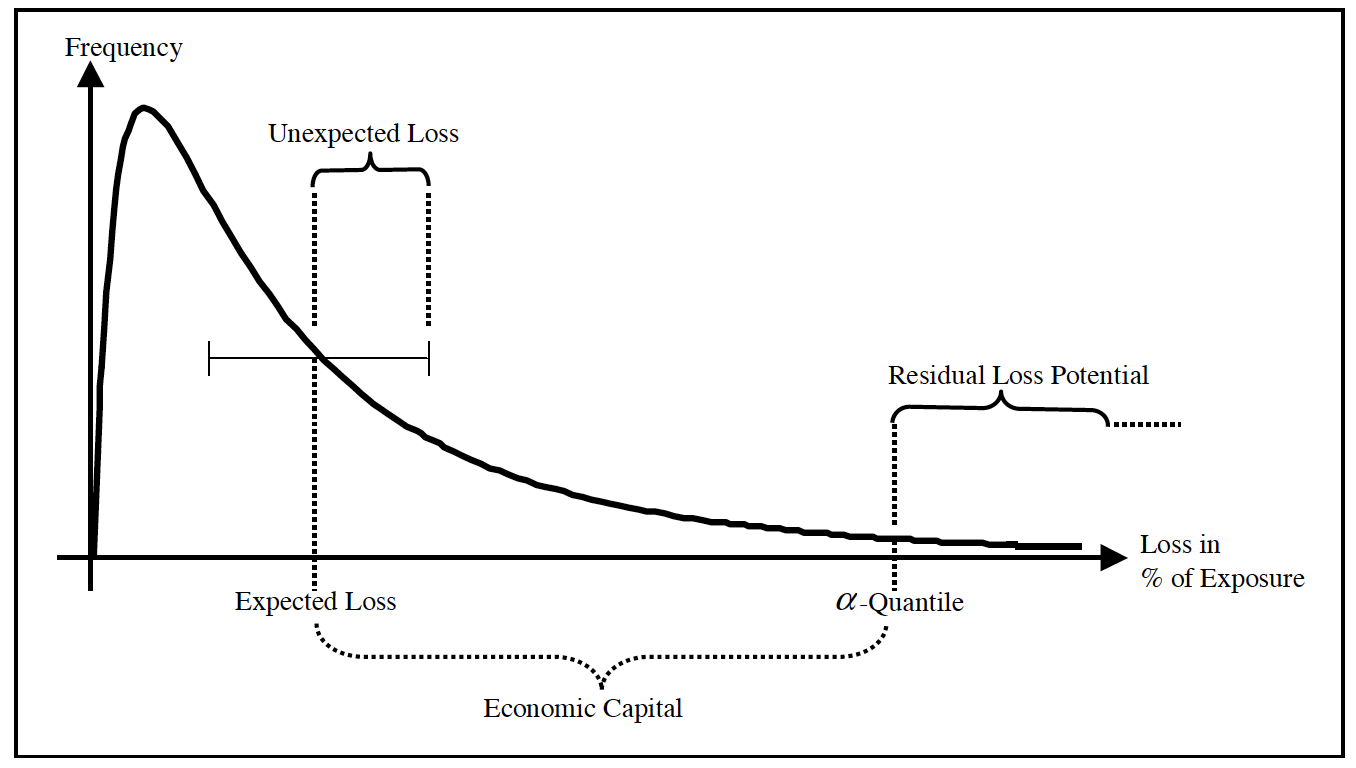
\includegraphics{images/varr.png}
\caption{\label{fig:"sd"}}
\end{figure}

\hypertarget{matriz-de-transicion}{%
\section{Matriz de transición}\label{matriz-de-transicion}}

La matriz de transición es un instrumento que se usa de manera fundamental en la metodología Credimetrics, que será desarrolada mas adelante. Como su nombre lo indica es una matriz, que además es cuadrada, el orden de la matriz depende de la cantidad de calificaciones que use la intitución financiera para calificar sus créditos, por ejemplo, si la intitucion usa 5 calificaciones, la matriz será una matriz cuadrada de orden 5

\begin{figure}
\centering
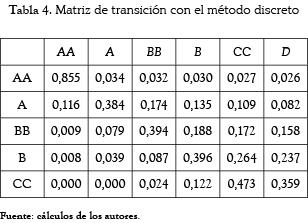
\includegraphics{images/mtr.jpg}
\caption{\label{fig:"sd"}}
\end{figure}

Ahora, la matriz de calificación indica la probabilidad de que un crédito con una calificación específica migre a otra calificación determinada, por ejemplo, por la imagen anterior, la probabilidad de que un crédito con calificación BB migre a una calificación B es de 0.188, es decir, se espera que el 18,8 \% de los créditos con calificación BB migren a la calificación B.

La matriz de transición también es conocida con el nombre de matriz de transición de probabilidad. Para que una matriz sea considerada como una matriz de transición crediticia, debe cumplir las siguientes propiedades:

\begin{itemize}
\item
  Todos sus elementos son no negativos y menores o iguales a 1
\item
  La suma de los elementos de cualquier columna es exactamente 1.
\end{itemize}

En general las matrices de transición esta intimamente relacionadas con las políticas internas de las instituciones financieras, y son generadas por metologías internas, y por lo general son calcúladas con simples medias exponenciales de migraciones.

\mainmatter

\hypertarget{scoring-de-credito}{%
\chapter{Scoring de crédito}\label{scoring-de-credito}}

Los métodos o modelos de credit scoring, a veces denominados score-cards o classifiers, son algoritmos que de manera automática evalúan el riesgo de crédito de un solicitante de financiamiento o de alguien que ya es cliente de la entidad. Tienen una dimensión individual, ya que se enfocan en el riesgo de incumplimiento del individuo o empresa, independientemente de lo que ocurra con el resto de la cartera de préstamos. Este es uno de los aspectos en los que se diferencian de otras herramientas de medición del riesgo de crédito, como son los modelos de cartera y los VaR marginales, que tienen en cuenta la correlación de la calidad crediticia de los deudores de una cartera de préstamos.

Los modelos de scoring fueron introducidos a partir del año 1970 en el análisis del otorgamiento del crédito, pero generalizados después de 1990 gracias al desarrollo estadístico y tecnológico. Entre los métodos para la construcción de modelos de scoring se pueden tener en cuenta como los más comunes, el modelo LOGIT, PROBIT, las Redes Neuronales y el Análisis Discriminante.

El resultado de la evaluación se refleja en la asignación de alguna medida que permita comparar y ordenar a los evaluados en función de su riesgo, a la vez que cuantificarlo. Por lo general, los modelos de credit scoring le asignan al evaluado un puntaje o score, o una calificación, clasificación o rating. Algunos métodos los asignan a grupos, en donde cada grupo tiene un perfil de riesgo distinto; sin embargo, en la práctica esto equivale a una calificación. A su vez, estos ordenamientos de los deudores permiten obtener estimaciones más concretas del riesgo; en general se busca obtener alguna estimación de la probabilidad de incumplimiento del deudor (PD, por probabilidad de default) asociada a su score, rating o calificación

\hypertarget{estructura-del-scoring-de-credito}{%
\section{Estructura del Scoring de Crédito}\label{estructura-del-scoring-de-credito}}

Cuando al plantear un modelo la variable dependiente o a explicar toma valores discretos, se emplean modelos de regresión discreta. El caso más simple se da cuando ella es binaria y toma los valores 0 o 1, y se puede estimar con distintos enfoques como el modelo de probabilidad lineal, análisis discriminante, los modelos de tipo probit y logit o con una regresión logística.

Sea \(Y\) una variable aleatoria binaria que toma el valor 1 si ocurre el evento (el deudor cumple con los pagos normalmente) y 0 si entra en mora, se cuenta con una muestra aleatoria de \(n\) observaciones, \(Y_i\), \(i: 1,...,n\), y se define como \(\Omega_i\) al conjunto de información relevante asociado con el individuo \(i\), que se utilizará para explicar a \(Y_i\).

Un modelo de elección binaria es un modelo de la probabilidad de ocurrencia del evento \(Y_i\) condicional en el conjunto de información \(\Omega_i\).

\begin{equation}
P_i = Pr(Y_i=1|\Omega_i)
\label{eq:ecuacion1} 
\end{equation}

Dado que \(Y_i\) toma los valores 0 y 1, la esperanza de \(Y_i\) condicional en \(\Omega_i\) es:

\begin{equation}
E(Y_i|\Omega_i)=(1*P_i)+(0*(1-P_i))=P_i=Pr(Y_i=1|\Omega_i)
\label{eq:ecuacion2}
\end{equation}

En consecuencia, cuando la variable a explicar es binaria, su esperanza condicional es la probabilidad condicional de ocurrencia del evento.

\hypertarget{el-modelo-de-probabilidad-lineal}{%
\section{El modelo de probabilidad lineal}\label{el-modelo-de-probabilidad-lineal}}

Supóngase que \(\Omega_i\) está constituido por un vector columna \(X_i\) compuesto por \(k\) variables explicativas, incluyendo a la ordenada al origen, \(\beta\) es un vector columna que contiene los parámetros correspondientes a las variables explicativas, y que se intenta modelar a la variable \(Y_i\) a través del modelo de probabilidad lineal, postulando la siguiente relación:

\[Y_i=\beta^TX_i+\epsilon_i,\quad\textrm{donde}\quad E(\epsilon_i|X_i)=0\quad \textrm{y}\quad E(\epsilon_i)=0 
\label{eq:ecuacion3}\]

y usando \eqref{eq:ecuacion2}

\[E(Y_i|X_i)=P_i=\beta^TX_i
\label{eq:ecuacion4}\]

El modelo de probabilidad lineal, como se observa en la ecuación \eqref{eq:ecuacion3}, implica estimar un modelo lineal en los parámetros para \(Y_i\). Los valores predichos deberían en su mayoría ubicarse en el intervalo \([0,1]\), pudiendo ser interpretados como la probabilidad de que la variable a explicar tome alguno de estos valores.

Mientras que su estimación e interpretación es simple, su utilización se ha visto desalentada por dos problemas en la metodología. En primer lugar, como la esperanza condicionada de \(Y_i\) es igual a la probabilidad condicionada de ocurrencia del evento (de \(Y_i=1\)), ella debería estar restringida al intervalo \([0,1]\). Sin embargo, el modelo lineal no impone ninguna restricción sobre \(\beta^TX_i\), suponiendo implícitamente que la variable dependiente puede tomar cualquier valor. Es por esto que el modelo puede estimar probabilidades negativas o mayores que uno, lo cual carece de significado económico. A su vez, el término de error de este modelo no es homocedástico, ya que la varianza condicional varía según las observaciones, por lo que las estimaciones de \(\beta\) no son eficientes.

Para resolver estos inconvenientes hay modelos econométricos, generalmente estimados por máxima verosimilitud, que tienen en cuenta la naturaleza discreta de la variable dependiente: se trata de los modelos de respuesta o elección binaria. Ellos utilizan ciertas funciones de distribución para la innovación, con el objetivo de limitar las probabilidades estimadas al intervalo {[}0,1{]}, las más usadas son la función de probabilidad acumulada normal estándar y la función logística. Cuando se usa la normal estándar se trata de un modelo probit, y logit cuando se usa la función logística.

\hypertarget{los-modelos-probit-y-logit.}{%
\subsection{Los modelos probit y logit.}\label{los-modelos-probit-y-logit.}}

El modelo probit es una de varias alternativas para estimar modelos de respuesta binaria. La idea consiste en utilizar una función de transformación F(x) que tenga las siguientes propiedades:

\[F(-\infty)=0, \quad F(\infty)=1\quad\textrm{y}\quad f(x)\equiv\frac{dF(x)}{dx}>0
\label{eq:ecuacion5}\]

\(F(x)\) es una función monótona creciente que mapea de la línea real al intervalo {[}0,1{]}. Varias funciones de distribución acumulada tienen estas propiedades: la normal, la logística, la de Cauchy y la de Burr, entre otras. Estas distintas alternativas para los modelos de respuesta binaria consisten en una función de transformación F(x) aplicada a una función índice que depende de las variables explicativas del modelo y que tiene las propiedades de una función de regresión, pudiendo ser lineal o no lineal.

La siguiente es una especificación general para cualquiera de los modelos de elección binaria:

\[E(Y_i|\Omega_i)=F(h(X_i))
\label{eq:ecuacion6}\]

Donde \(h\) es la función índice.

Si bien \(h\) puede ser cualquier función, en general se usa una función lineal, es decir:

\[E(Y_i|\Omega_i)=F(\beta^TX_i)
\label{eq:ecuacion7}\]

Por lo cual el modelo de elección binaria es simplemente una transformación no lineal de una regresión lineal, y si bien \(\beta^TX_i\) puede tomar cualquier valor sobre la línea real, \(F(\beta^TX_i)\) está limitado al intervalo {[}0,1{]}. En el modelo probit, la función de transformación \(F(x)\) es la función de distribución acumulada normal estándar, y por definición satisface las condiciones impuestas en \eqref{eq:ecuacion5}. En este caso, el modelo de elección binaria puede escribirse de la siguiente manera:

\[P_i=E(Y_i|\Omega_i)=F(\beta^TX_i)=\Phi(\beta^TX_i)=\int_{-\infty}^{\frac{\beta^TX_i}{\sigma}}\frac{e^{\frac{-s^2}{2}}}{\sqrt{2\pi}}ds
\label{eq:ecuacion8}\]

Cuando se trata del modelo logit, \(F(x)\) es la función logística y el modelo de respuesta binaria se escribe como:

\[P_i=E(Y_i|\Omega_i)=F(\beta^TX_i)=\Phi(\beta^TX_i)=\frac{e^{\beta^TX_i}}{1+e^{\beta^TX_i}}
\label{eq:ecuacion9}\]

Los modelos probit y logit pueden ser derivados de otro modelo que introduce una variable no observada o latente \(y^*\), de la siguiente manera. Sea:

\[y^*_i=\beta^TX_i+\epsilon_i, \quad \textrm{con} \quad \epsilon_i\sim iid(0,1)
\label{eq:ecuacion10}\]

Si bien \(y^*\) no se observa, decimos que:

\[Y_i=1\quad\quad\textrm{si} \quad y^*>0 \quad \textrm{y} \quad Y_i=0\quad\quad\textrm{si} \quad y^*<0
\label{eq:ecuacion11}\]

Luego, la probabilidad que \(Y_i=1\) viene dada por:

\begin{equation} \label{eq1}
\begin{split}
P(Y_i=1) & = P(y_i^*>0)=P(\beta^TX_i+\epsilon_i>0)= 1-P(\beta^TX_i+\epsilon_i\leq 0)\\
& =1-P(\epsilon_i\leq -\beta^TX_i)\\
 & = 1-F(-\beta^TX_i)=F(\beta^TX_i)
\end{split}
\end{equation}

ya que se supone que \(\epsilon_i\) tiene una distribución simétrica. Cuando \(\epsilon_i \sim N(0,1)\) y \(F\) es \(\Phi\), la función de distribución de probabilidades acumuladas normal estándar y se trata del modelo probit, mientras que si F es la función logística se trata de un modelo logit y su densidad también es simétrica alrededor de cero.

\hypertarget{estimacion-de-los-modelos-logit-y-probit}{%
\subsection{Estimación de los modelos logit y probit}\label{estimacion-de-los-modelos-logit-y-probit}}

La estimación de estos modelos se hace por el método de máxima verosimilitud. Con métodos numéricos se buscan los valores de \(\beta\) que maximizan la siguiente función logarítmica de verosimilitud:

\[l(\beta)=\sum^{n}_{i=1}\big{(}Y_ilog\big{(}F\big{(}\beta^TX_i\big{)}\big{)}+\big{(}1-Y_i\big{)}log\big{(}1-F\big{(}\beta^TX_i\big{)}\big{)}\big{)}
\label{eq:ecuacion12}\]

Las condiciones de primer orden para un máximo en \eqref{eq:ecuacion12} son:

\[\sum_{i=1}^n\frac{(Y_i-\hat{F_i)}\hat{f_i}X_{ij}}{\hat{F_i}(1-\hat{F_i})}=0,\quad j=1,...,k
\label{eq:ecuacion13}\]

donde \(\hat{F_i}\equiv F_i(b^TX_i) \quad \textrm{y} \quad \hat{f_i}\equiv f_i(b^TX_i)\)

Los modelos probit, logit y otros tipos de modelos de respuesta binaria satisfacen las condiciones de regularidad necesarias para que las estimaciones de los parámetros sean consistentes y asintóticamente normales, con la matriz de covarianzas asintótica dada por la inversa de la matriz de información.

\hypertarget{interpretacion-del-modelo}{%
\subsection{Interpretación del modelo}\label{interpretacion-del-modelo}}

En el contexto de los modelos de credit scoring se puede asociar \(\beta^TX_i\) a la calidad crediticia del individuo (variable latente o no observada). Cambiando su denominación por \(Z_i\), esta variable representa la calidad crediticia del individuo, que se puede suponer el resultado de una función lineal en sus parámetros, como por ejemplo:

\[Z_i=\beta_0+\beta_1X_{1j}+\beta_2X_{2j}+...+\epsilon_i
\label{eq:ecuacion14}\]

Las estimaciones de los parámetros \(\beta_j\) se obtienen por máxima verosimilitud como se explicó en los párrafos anteriores, y las variables \(X_j\) contienen la información de los deudores. Habiendo obtenido las estimaciones \(b_j\), el modelo empírico con el que trabajará el analista de riesgo es,

\[Z_i=\beta_0+\beta_1X_{1j}+\beta_2X_{2j}+\beta_3X_{3j}
\label{eq:ecuacion15}\]

cuando se trata de un modelo que emplea cinco variables (\(j=5\)). La variable \(z_i\) es el score estimado del deudor, una medida de su calidad crediticia obtenida a partir de los parámetros estimados y de su propia información. Este score, aplicado a las funciones de distribución de probabilidades acumuladas normal o logística, permite conocer la probabilidad de incumplimiento y en consecuencia el riesgo del deudor.

\hypertarget{relacion-entre-el-score-y-el-riesgo}{%
\subsection{Relación entre el score y el riesgo}\label{relacion-entre-el-score-y-el-riesgo}}

Habiendo definido al score, como \[P(Y_i=1)=F(Z_i)\] y \[P(Y_i=0)=1-F(Z_i)\]

donde queda claro que cambios en \(Z_i\) implican cambios en la probabilidad de incumplimiento (PD) del individuo. La relación entre score y riesgo (la PD) no es lineal, por lo que el cambio en el riesgo derivado de un cambio en el score depende de los valores que este último tome. Para valores del score muy bajos, un aumento en el mismo produce una rápida subida en la probabilidad de cumplimiento y una rápida disminución de la PD, mientras que para valores del score altos, una mejora en el mismo hace que la probabilidad de incumplimiento aumente poco y genera una leve caída en el riesgo. Es decir, cuanto mayor es el score, menor es la caída en el riesgo derivada de un aumento en el primero.

\hypertarget{uso-de-modelos-lineales-para-la-seleccion-de-variables-metodos-de-busqueda-secuencial.}{%
\subsection{Uso de modelos lineales para la selección de variables (Métodos de búsqueda secuencial).}\label{uso-de-modelos-lineales-para-la-seleccion-de-variables-metodos-de-busqueda-secuencial.}}

Los métodos de búsqueda secuencial tienen en común la aproximación general de estimación de las ecuaciones de regresión con un conjunto de variables y a continuación añadir o eliminar selectivamente variables hasta que se consiga alguna medida ó criterio. Esta aproximación proporciona un método objetivo de selección de variables que maximizan la predicción con el número más pequeño de variables empleadas. Existen dos tipos de aproximaciones de búsqueda secuencial: (1) la estimación por etapas, y (2) la eliminación progresiva y regresiva. En cada aproximación, se valoran las variables individualmente en función de su contribución a la predicción de la variable dependiente y se añaden o eliminan según su contribución relativa.

\hypertarget{estimacion-por-etapas-paso-a-paso-o-stepwise}{%
\subsubsection{Estimación por etapas (paso a paso o stepwise)}\label{estimacion-por-etapas-paso-a-paso-o-stepwise}}

La estimación por etapas es quizá la aproximación más popular para seleccionar variables. Esta aproximación permite examinar la contribución de cada variable predictor al modelo de regresión. Se considera la inclusión de cada variable antes de desarrollar la ecuación. Se añade primero la variable independiente con la contribución más grande. Las variables independientes se seleccionan entonces para la inclusión basada en su contribución incremental sobre la(s) variable(s) ya existente(s) en la ecuación. Las cuestiones específicas en cada etapa son:

\begin{enumerate}
\def\labelenumi{\arabic{enumi}.}
\item
  Empezar con el modelo de regresión simple en el cual sólo se utiliza la única variable predictor que es la que se muestra más altamente correlacionada con la variable criterio. La ecuación sería \(Y= \beta_0 Q + \beta_1X_1\).
\item
  Examinar los coeficientes de correlación parcial para encontrar una variable predictor adicional que explique además de una parte significativa, la mayor parte del error que queda de la primera ecuación de regresión.
\item
  Recalcular la ecuación de regresión utilizando las dos variables predictor, y examinar el valor parcial \(F\) de la variable original del modelo para ver si todavía realiza una contribución significativa, dada la presencia de la nueva variable predictor. Si no lo hace, eliminamos la variable. Esta capacidad de eliminar variables presentes en el modelo distingue el modelo por etapas de los modelos de adición progresiva/eliminación regresiva. Si las variables originales todavía representan una contribución significativa, la ecuación sería \(Y = \beta_0 + \beta_1X_1 + \beta_2X_2\).
\item
  Continúa este procedimiento examinando todos las variables independientes no presentes en el modelo para determinar si deberían incluirse en la ecuación. Si se incluye una nueva variable independiente, hay que examinar todos los predictores previamente incluidos en el modelo para juzgar si se deben mantener. Existe un sesgo potencial en el procedimiento por etapas que resulta de considerar solo una variable a seleccionar cada vez. Supongamos que las variables \(X_3\) y \(X_4\) explicaran conjuntamente una parte significativa de la varianza (cada una considerando la presencia de la otra), pero no son significativas por sí solas. En esta situación, ninguna debería ser considerada para el modelo final.
\end{enumerate}

\hypertarget{la-adicion-progresiva-forward-y-la-eliminacion-regresiva-backward}{%
\subsubsection{La adición progresiva (forward) y la eliminación regresiva (backward)}\label{la-adicion-progresiva-forward-y-la-eliminacion-regresiva-backward}}

La adición progresiva y la eliminación regresiva son fundamentalmente procesos de ensayo y error para buscar los mejores estimadores de la regresión. El modelo de adición progresiva es similar al procedimiento por etapas arriba explicada, mientras que el procedimiento de eliminación regresiva implica calcular una ecuación de regresión con todas las variables independientes, para a continuación ir eliminando las variables independientes que no contribuyan significativamente. La distinción principal de la aproximación por etapas respecto de los procedimientos de adición progresiva y eliminación regresiva es su capacidad de añadir o eliminar las variables en cada etapa. Una vez que se añade o elimina una variable en los esquemas de adición progresiva o eliminación regresiva, no existe posibilidad de revertir la acción posteriormente.

\hypertarget{advertencias-sobre-los-metodos-de-busqueda-secuenciales}{%
\subsubsection{Advertencias sobre los métodos de búsqueda secuenciales}\label{advertencias-sobre-los-metodos-de-busqueda-secuenciales}}

El investigador debe ser consciente de dos advertencias cuando se usa cualquier procedimiento de búsqueda secueneial. En primer lugar, la multicolinealidad entre variables independientes puede tener un impacto sustancial sobre la especificación final del modelo. Examinemos esta situación con dos variables altamente correlacionadas que tienen similares correlaciones con la variable independiente. El criterio de inclusión o eliminación en estas aproximaciones es maximizar el incremento de potencia predictiva de la variable adicional. Si una de estas variables entra en el modelo de regresión, es muy probable que la otra variable también entre, dado que estas variables están altamente correlacionadas y existe poca varianza singular para cada variable por separado.

Por esta razón, se deben evaluar los efectos de la multicolinealidad en la interpretación del modelo y examinar las correlaciones directas de todas las variables independientes potenciales. Esto ayudará a evitar concluir que las variables independientes que no entren en el modelo no sean trascendentes cuando en realidad están altamente relacionadas con la variable dependiente, pero también correlacionadas con las variables ya existentes en el modelo. Aunque las aproximaciones de búsqueda secueneial maximizarán la capacidad predictiva del modelo de regresión, el investigador debe ser cuidadoso en la interpretación del modelo. Una segunda advertencia pertenece principalmente al procedimiento por etapas. En esta aproximación, los test de significación múltiple se realizan en el proceso de estimación del modelo. Para asegurar que la tasa de error conjunto a lo largo de todos los test de significación es razonable, el investigador debería emplear umbrales muy conservadores (por ejemplo, 0,01) al añadir o sacar las variables.

\mainmatter

\hypertarget{creditrisk}{%
\chapter{CreditRisk+}\label{creditrisk}}

\textbf{CreditRisk+} es un modelo de impago en el que se parte de la idea de que los eventos de incumplimiento de los diferentes deudores son eventos \emph{Bernoulli independientes}. Sin embargo, es importante tener en cuenta que los eventos de incumplimiento de deudores ocurren de manera causística en el tiempo y es imposible pronosticar el momento preciso en el que ocurrirán dichos eventos y el número de eventos que sucederán en un cierto intervalo de tiempo.

El desarrollo de una teoría estadística que explique estos procesos, dentro del contexto de riesgo crediticio, comienza considerando el caso simple de una cartera de créditos que incluye a \(N\) deudores, a cada uno de los cuales se les puede asociar una \emph{probabilidad fija de incumplimiento}; es decir, se conoce: \[p_i=\textrm{Probabilidad de incumplimiento del deudor } i\]

La distribución de pérdidad que puede resultar del incumplimiento de los deudores de todo el portafolio la obtiene \textbf{CreditRisk+} de manera indirecta, a través de las funciones de probabilidad, y procede en dos pasos. Primero, obtenemos la función generadora de probabilidad (FGP) del número de incumplimientos y después, haciendo un supuesto sobre el nivel de pérdidas asociadas al incumplimiento de cada deudor, obtiene la FGP las pérdidas que puede ceder la cartera. A continuación se obtiene la primera para el caso simple bajo consideración.

\hypertarget{la-distribucion-del-numero-de-incumplimientos-con-probabilidades-de-impago-fijas.}{%
\section{La distribución del número de incumplimientos con probabilidades de impago fijas.}\label{la-distribucion-del-numero-de-incumplimientos-con-probabilidades-de-impago-fijas.}}

La FGP de números de incumplimientos se define como: \[F(s)=\sum_{n=0}^{\infty}Prob(n \textrm{ incumplimientos})\textrm{x}s^n\]

Si la cartera tuviera un solo deudor, lo único que puede suceder es que él cumpla o incumpla. Por lo tanto, la FGP de incumplimientos para un solo deudor es simplemente:\[F_i(s)=(1-p_i)s^0+p_i(s-1)=1+p_i(s-1)\]

Como se considera que los eventos de incumplimiento son independientes, la FGP de toda la cartera es el producto de las FGP individuales, es decir:\[F(s)=\prod_{i=1}^NF_i(s)=\prod_{i=1}^N\big{[}1+p_i(s-1)\big{]}\]
Aplicando logaritmo a ambos lados de la expresión, se obtiene:\[Ln(F(s))=\sum_{i=1}^NLn\big{[}1+p_i(s-1)\big{]}\]
Generalmente, las probabilidades de incumplimiento de obligaciones crediticias a nivel individual son pequeñas y, por lo tanto, las potencias de estas son más pequeñas y pueden ser ignoradas.

Esto implica que para los valores pequeños de \(p_i\):\[Ln\big{[}1+p_i(s-1)\big{]}\approx p_i(s-1)\]
Lo anterior es el gran supuesto de \textbf{CreditRisk+}, que inituitivamente dice que mientras la probabilidad de incumplimiento se \(p_i\) sea ``pequeña'', se puede ignorar el hecho de que un deudor no puede incumplir más que una sola vez. Haciendo esta sustitución, se obtiene:\[Ln(F(s))=\sum_{i=1}^Np_i(s-1)\]
Lo anterior conduce directamente a: \[F(s)=e^{\sum_{i=1}^Np_i(s-1)}=e^{\mu(s-1)};\textrm{ donde } \mu=\sum_{i=1}^Np_i\]

La FGP corresponde a la FGP de la distribución de \emph{Poisson} con parámetro \(\mu\), a continuación se comprueba esto, usando el desarrollo de Taylor, es decir:\[F(s)=\sum_{n=}^\infty\mu^ne^{-\mu}s^n\]
Por lo tanto, bajo el supuesto de que las probabilidades de incumplimientos son bajas, obtenemos que:\[Prob(\textrm{ número incumplimientos }=n)=\frac{1}{n!}\mu^ne^{-\mu}\]

En la expresión anterior, `\(\mu\)' es la \emph{tasa promedio de incumplimiento} y es el único parámetro de la distribución. Como ``\(N\)'', la distribución es independiente del número de deudores y de las probabilidades individuales de impago, siempre y cuando sean ``uniformemente pequeñas''.

Para concluir con este tema, es impotante hacer hicapié en que el supuesto clave que permite llegar a la distribución Poisson es cuando un número no-negativo ``\(y\)'' es muy pequeño (\(y\approx 0\)), se puede utilizar la aproximación ``\(Ln(1+y)\approx y\)''. Esta forma exponencial de la FGP de la distribución de Poisson, es la clave de la facilidad de cálculo que tiene \textbf{CreditRisk+}.

Además, es necesario señalar que en todo el análisis anterior hay implícito un período de tiempo que está relacionado con el parámetro de la distribución. Así, la distribución obtenida debe interpretarse de la misma manera, es decir:\[\frac{1}{n!}\mu^ne^{-\mu}=\textrm{ Probabilidad de que ocurran } n \textrm{ incumplimientos }\]

\hypertarget{la-agrupacion-por-bandas-de-exposicion-de-las-perdidas}{%
\section{La agrupación por bandas de exposición de las pérdidas}\label{la-agrupacion-por-bandas-de-exposicion-de-las-perdidas}}

Dado que pueden existir varios deudores que implican niveles de pérdidas semejantes, \textbf{CreditRisk+} empieza por agrupar a los deudores por bandas de exposición iguales. Aunque esta agrupación introduce errores de rodondeo en la estimación de la distribución, facilita mucho el desarrollo del modelo y reduce significativamente el número de datos requeridos para realizar los cálculos. Además, si el número de niveles de exposición es grande y el ancho de las bandas es pequeño, en relación con el tamaño de exposición promedio de la cartera, se puede demostrar que el error introducido es despreciable. De hecho, en la práctica es muy difícil determinar \emph{a priori} el nivel de exposición y, por lo tanto, este no debe representar un elemento crítico en la estimación del riesgo total de la cartera.

Así, supóngase que la pérdida esperada por deudor que cae en impago es una proporción fija ``\(\lambda_i\)'' del monto total ``\(D_i\)'' que debe el deudor ``\(i\)''. A su vez, para mantener la elegancia del modelo, supóngase que el nivel de exposición que representa el deudor para el acreedor ``\(L_i\)'' es un múltiplo entero de una únidad fija de pérdida ``\(L\)''. Estos múltiplos enteros de \(L\) reciben el nombre de ``\emph{niveles de exposición estándar}''. Así la pérdida que puede representar el incumplimiento del deudor ``\(i\)'' para el acreedor, se mide en términos de múltiplos de ``\(v_i\)'', de la únidad fija de pérdida \(L\), y es simplemente la cantidad siguiente:\[v_i=\textrm{ Redondeo }\bigg{(}\frac{\lambda D_i}{L}\bigg{)}\]
De esto se obtiene el nivel estándar de exposición que representa cada deudor para el acreedor, mediante la identidad siguiente:\[L_i=L_{v_i}\]

\hypertarget{la-determinacion-de-la-distribucion-de-perdidas-de-la-cartera.}{%
\section{\texorpdfstring{La determinación de la \emph{distribución de pérdidas} de la cartera.}{La determinación de la distribución de pérdidas de la cartera.}}\label{la-determinacion-de-la-distribucion-de-perdidas-de-la-cartera.}}

El último paso es encontrar la \emph{la distribución de pérdidas de la cartera}, para lo cual se procede de la misma manera, es decir, encontar la FGP de dicha distribución. Nótese que la distribución de pérdidas es necesariamente diferente a la del número de impagos, ya que puede resultar un cierto nivel de pérdidas con diferentes combinaciones de incumplimientos de deudores. Por ejemplo una pérdida de \(100.000\) dolares puede ser la consecuencia del incumplimiento que debe esta cantidad o del incumplimiento de \(10\) de deudores que deben \(10.000\) dolares cada uno. Además, el conocimiento de la forma en que están distribuidos los diferentes niveles de exposición entre los diferentes deudores que componen la cartera es indispensable para poder obtener la distribución de pérdidas. Contrario a lo que sucede con las diferencias entre probabilidades de incumplimiento individuales, que son pequeñas aun en términos relativos y por lo tanto no afectan la distribución del número de incumplimiento, las diferencias en los niveles de exposición a los deudores representados en la cartera si son significativos y, por lo tanto, la distribución de pérdidas resultante no tiene por que ser \emph{Poisson}. Sin embargo, aunque no se va a poder obtener una fórmula explícita de la distribución de pérdidas, se verá que es posible obtener una expresión cerrada sencilla de la FGP, que se presta fácilmente al cálculo de las probabilidades correspondientes.

Así, recordemos que la FGP de las pérdidas es: \[G(s)=\sum_nProb(\textrm{ Pérdida acumulada}=n\textrm{x}L)S^n\]

Sea ``\(G_j\)'' la FGP de las pérdidas de la banda ``\(j\)'', la probabilidad de que se pierda \(n\times v_j\) unidades en la banda ``\(j\)'' es igual a la probabilidad de que ``\(n\)'' deudores de esta banda incumplan, y ya se sabe que el incumplimiento de estos deudores sigue una distribución de \emph{Poisson}, es decir:\[\textrm{ Prob. de }n\textrm{ incumplimientos en la banda }j=\frac{1}{n!}\mu_j^ne^{-\mu_j}\]

Por lo tanto:\[G_j(s)=\sum_{n=0}^\infty \frac{1}{n!}\mu_j^ne^{-\mu_j}s^{nv_j}=e^{-\mu_j}\sum_{n=0}^\infty \frac{1}{n!}(\mu_js^{v_j})^n=e^{-\mu_j}e^{\mu_js^{v_j}}=e^{\mu_j(s^{v_j}-1)}\]

Suponiendo independencia de eventos de incumplimientos, las pérdidas asociadas a cada banda tambien serán independientes. En este caso, la FGP de las pérdidas de la cartera de crédito es la suma de las pérdidas ocurridas en cada banda, que por propiedades de las funciones generadoras de probabilidad es el producto de las FGP de las bandas:\[G(s)=\prod_jG_j(s)=\prod_{j=1}^me^{\mu_j(s^{v_j}-1)}=e^{\sum_{j=1}^m\mu_j(s^{v_j}-1)}\]es decir:\[G(s)=e^{\sum_{j=1}^m\mu_j(s^{v_j}-1)}\]

\hypertarget{obteniendo-la-distribucion-de-las-perdidas}{%
\section{Obteniendo la distribución de las pérdidas}\label{obteniendo-la-distribucion-de-las-perdidas}}

Aunque a diferencia de la distribución del número de incumplimientos, en el caso de las pérdidas no se sabe la forma de la distribución, la probabilidad de que se pierdan \(n\) unidades de \(L\) en la cartera total de créditos se puede obtener mediante la expansión de Taylor de la expresión anterior; es decir: la probabilidad de que se pierdan \(n\) unidades \(L\) es el coeficiente de \(s^n\) en la expansión de Taylor. El desarrollo se facilita definiendo el polinomio siguiente:\[P(s)=\frac{1}{\mu}\sum_{j=1}^m\mu_js^{v_j}=\frac{\sum_{j=1}^m\frac{\epsilon_j}{{v_j}}s^{v_j}}{\sum_{j=1}^m\frac{\epsilon_j}{{v_j}}}\] donde \(\epsilon_j\) es la perdida esperada de la banda \(j\) y \(v_j\) es la exposición común que comparten los deudores de la banda \(j\).

Con esto, la FGP de pérdidas se puede expresar de la forma siguiente:\[G(s)=e^{\sum_{j=1}^m\mu_j(s^{v_j}-1)}=e^{\mu[P(s)-1]}=F[P(s)]\]
La función generadora de probabilidades de las pérdidas comprende dos fuentes de incertidumbre, a saber: el comportamiento \emph{Poisson} del número de incumplimiemntos y la aleatoriedad de las pérdidas dado incumplimiento, que está asociado a los distintos niveles de exposición del acreedor a los diferentes deudores. Notese que la única información requerida para obtener la distribución de pérdidas es \(\epsilon_j\) y \(v_j\), estas parejas representan un número de datos significativamente menor, que si tuviera que manejar información semejante por cada deudor, aun para carteras con un número muy grandes de créditos.
Para encontrar la distribución de pérdidas, se parte de la expresión:\[G(s)=\sum_n\textrm{ Prob(pérdidas acumuladas}=n\times L)S^n \].

Tomando la expansión de Taylor para \(G(s)\), la probabilidad de pérdida de \(nL\) unidades es\[P_n(L)=\frac{1}{n!}\frac{d^nG(s)}{ds^n}\bigg{|}_{s=0}\]. En el apéndice A 4.1 del manual de CreditRisk+ se deduce una fórmula recursiva sencilla para obtener estas probabilidades, las cuales es:\[P_n(L)=\sum_{j|v_j\le n}\frac{\epsilon_j}{n}P_{n-v_j}(L)=\frac{1}{n}\sum_{j|v_j\le n}\epsilon_jP_{n-v_j}(L)\]
donde \(P_0(L)=e^{-\mu}\) donde \(\mu=\sum_{j=1}^m\mu_j\)

\hypertarget{obtencion-del-var}{%
\section{Obtención del VaR}\label{obtencion-del-var}}

Para obtener el VaR de una cartera de créditos bajo el esquema de CreditRisk+, simplemente se obtiene la distribución
de probabilidad acumulada de las pérdidas y, una vez decidido el nivel de confianza \(\alpha\) con el que se quiere trabajar se lee de la tabla el número de unidades estándar de pérdidas que corresponden a una probabilidad acumulada de de pérdida \(1-\alpha\). El paso final es convertir las unidades estándar de pérdida a unidades manetarias, multiplicando las unidades de pérdidas correspondientes al nivel de confianza escogido, por la unidad de pérdida \(L\).

\mainmatter

\hypertarget{creditmetrics}{%
\chapter{CreditMetrics}\label{creditmetrics}}

Mientras que en el caso de \textbf{CredictRisk+} se usa un enfoque actuarial mediante el cual se llega ha obtener una forma explícita de la distribución de pérdidas a través de la función generadora de probabilidades, en el caso de \textbf{CredictMetrics}, aunque en teoría existe una representación explícita de la distribución de pérdidas, su obtención supera la capacidad de cálculo disponible en un computador convencional, y por lo tanto, está se estima a través de un proceso de simulación de \emph{MonteCarlo}, otra caractéristica importante es que \textbf{CreditMetric} hace referencia, y utiliza extensamente, información que solo esta disponible en los mercados en desarrollo, aunque esto no impide que se aplique en los mercados emergentes si se hacen las edecuaciones correspondientes.

Para la explicación de esta metodología usamos como guía el documento técnico de \textbf{CreditMetrics}. Iniciaremos con el caso más sencillo en el cual nuestrea cartera de créditos esta integrada por un único crédito para luego generalizar el procedimiento a una cartera que puede incluir cualquier número \(N\) de créditos. Pero primero establescamos los elementos básicos que usaremos en esta metodología.

\hypertarget{elementos-de-credimetrics}{%
\section{\texorpdfstring{Elementos de \textbf{Credimetrics}}{Elementos de Credimetrics}}\label{elementos-de-credimetrics}}

\begin{itemize}
\item
  \emph{Conceptos relevantes al riesgo de crédito}: probabilidades de incumplimiento, patrones de migración entre los distintas clasificaciones que posean los clientes, umbrales que separen las calificaciones, el valor de los créditos, la tasa de recuperación en caso de incumplimiento de las calificaciones crediticia.
\item
  Información del mercado en general: Tales como datos sobre las calificaciones e indicadores sobre su calidad.
\item
  Información generada internamente por las instituciones que se pueda mapear a los estándares del mercado.
\end{itemize}

Históricamente Credimetrics fue desarrollado para abordar el problema de medir el riesgo de crédito de que los emisores que colocan papel que se negocia en el mercado de los Estados Unidos incumplan sus compromisos. En general, los elementos que son necesarios en esta metodología están disponibles en mercados desarrollados, pero las intituciones financieras pueden crear procedimientos y metodologías internas para lograr suplir la falta de información. Los elementos clave del sistema son:

\begin{itemize}
\item
  Las calificaciones que otorgan las instituciones financieras a los distintos elementos que conforman su portafolio.
\item
  Las diferencias de riesgo que expresan las distintas calificaciones.
\item
  Información sobre la tasa de recuperación sobre créditos que caen en la cartera vencida.
\end{itemize}

Una característica importante de las calificaciones emitidas es que ellas aportan de manera implícita piezas clave para la evaluación del riesgo de crédito, como por ejemplo:

\begin{itemize}
\item
  Probabilidades de incumplimiento históricas asociadas a cada calificación, así como las probabilidades de transición entre las categorías.
\item
  Las distintas tasas de interés asociadas a cada categoría.
\end{itemize}

Otra parte fundamental del análisis es la cantidad que se espera recuperar en caso de que el crédito caiga en la cartera de vencidos. Aunque si el sistema de calificación es robusto raramente se espera que un crédito que halla pasado a la cartera de vencido este en una calificación alta. Pero al final, la calificación no solo depende del sistema interno de la institución, sino también de la garantías que ofresca el crédito.

En general, todos los requerimientos están entrelazados, por ejemplo las calificaciones que se otorgan dependen de cosas como: historial de incumplimiento, garantías, utilidades de los créditos en los últimos años, el país de origen, entre otros.

A manera de ilustración se presenta una matriz de transición publicada por Standard \& Poor's en Abril de 1966. En ella se aprecian las probabilidades de transición de que un bono que se encuentra en una calificación dada migre a otra calificación, por ejemplo en la tabla se aprecia que la probabilidad de que un bono que esta en la calificación BB migre a una calificación C es de un 1\%.

\begin{longtable}[]{@{}ccccllll@{}}
\toprule
Calificación inicial & AAA & AA & A & BBB & BB & B & C\tabularnewline
\midrule
\endhead
AAA & 90.81 & 8.33 & 0.68 & 0.06 & 0.12 & 0.00 & 0.00\tabularnewline
AA & 0.70 & 90.65 & 7.79 & 0.64 & 0.06 & 0.14 & 0.02\tabularnewline
A & 0.09 & 2.27 & 91.05 & 5.52 & 0.74 & 0.26 & 0.01\tabularnewline
BBB & 0.02 & 0.33 & 5.95 & 86.93 & 5.30 & 1.17 & 0.12\tabularnewline
BB & 0.03 & 0.14 & 0.67 & 7.73 & 80.53 & 8.84 & 1.00\tabularnewline
B & 0.00 & 0.11 & 0.24 & 0.43 & 6.48 & 83.46 & 4.07\tabularnewline
C & 0.22 & 0.00 & 0.22 & 1.30 & 2.38 & 11.24 & 64.86\tabularnewline
\bottomrule
\end{longtable}

Las tasas de recuperación de los créditos como ya se menciono son fundamentales, y no son únicamente proporcionadas por las instituciones financieras, estas pueden recurrir a terceros por las calificaciones de los créditos. A continuación se presenta una tabla que muestra las tasas de recuperación de créditos elaboradas por Moody's y otros académicos.

\begin{longtable}[]{@{}ccc@{}}
\toprule
Prelación & Media (\%) & Desv. Std (\%)\tabularnewline
\midrule
\endhead
Senior Garantizada & 53.80 & 26.86\tabularnewline
Senior sin Garantía & 51.13 & 25.45\tabularnewline
Senior Subordinado & 38.52 & 23.81\tabularnewline
Subordinada & 32.74 & 20.18\tabularnewline
Junior Subordinada & 17.09 & 10.90\tabularnewline
\bottomrule
\end{longtable}

Una acotación interesante, es que originalmente credimetrics esta direccionada a medir el riesgo de crédito de una cartera de bonos. Sin embargo puede ser aplicado a distintos tipos de posiciones que involucren riesgo de crédito, como por ejemplo: posiciones cortas en divisas, futuros, opciones o como es el caso de interés, créditos tradicionales. Ahora, daremos el ejemplo de credimetrics usando un único crédito.

\hypertarget{el-caso-de-un-solo-credito}{%
\section{El caso de un solo crédito}\label{el-caso-de-un-solo-credito}}

Una vez descrito los elementos necesarios para esta metodología vamos a empezar por realizar los pasos que son necesarios para la medición del riesgo de crédito de una cartera de un solo activo. Utilizaremos un ejemplo parecido al que procede del documento de Credimetrics con la diferencia que ellos usan un bono y nosotros un crédito personal. Los tres pasos a realizar son:

\begin{itemize}
\item
  Dependiendo de la calificación del bono, se obtiene la probabilidad de que migre hacia un estado de migración diferente.
\item
  Se calcula el saldo o la exposición de los créditos.
\item
  Se aplican las probabilidades de migración a la expoción que posee el crédito para obtener la distribución de probabilidad de pérdida o perfil de riesgo del instrumento y las estadísticas que corresponden, es decir, la pérdida esperada, su varianza o desviación estándar, su VaR con un nivel de confianza deseado, entre otros.
\end{itemize}

\hypertarget{ejemplo-1}{%
\subsection{Ejemplo 1}\label{ejemplo-1}}

Supongamos que tenemos un crédito con calificación BB con exposición de 250, la institución financiera posee la siguiente información sobre las probabilidades calificación de los créditos que están en una calificación BB:

\begin{longtable}[]{@{}cc@{}}
\toprule
Calificación & Probabilidad de transición (\%)\tabularnewline
\midrule
\endhead
AAA & 4\tabularnewline
AA & 5\tabularnewline
A & 9\tabularnewline
BBB & 15\tabularnewline
BB & 44\tabularnewline
B & 18\tabularnewline
CCC & 5\tabularnewline
\bottomrule
\end{longtable}

También la institución cuenta con las pérdidas esperadas por calificación (las cuales representan la inversa aritmética de las tasas de recuperación en caso de que el crédito caiga en default o mora)

\begin{longtable}[]{@{}cc@{}}
\toprule
Calificación & Pérdida esperada (\%)\tabularnewline
\midrule
\endhead
AAA & 0.1\tabularnewline
AA & 3\tabularnewline
A & 5\tabularnewline
BBB & 9\tabularnewline
BB & 18\tabularnewline
B & 25\tabularnewline
CCC & 40\tabularnewline
\bottomrule
\end{longtable}

Ya con esta información podemos establecer una tabla con la pérdida esperada del crédito en las distintas calificaciones, la cual es:

\begin{longtable}[]{@{}ccc@{}}
\toprule
Calificación & Pérdida esperada del Crédito & Proababilidad\tabularnewline
\midrule
\endhead
AAA & 0.25 & 4\tabularnewline
AA & 7.5 & 5\tabularnewline
A & 12.5 & 9\tabularnewline
BBB & 22.5 & 15\tabularnewline
BB & 45 & 44\tabularnewline
B & 62.5 & 18\tabularnewline
CCC & 100 & 5\tabularnewline
\bottomrule
\end{longtable}

De esta forma para obtener la pérdida esperada se procede a multiplicar la pérdida esperada de una calificación por la probabilidad de que el crédito caiga en la respectiva calificación y luego se realiza la suma global, de la siguiente forma:

\begin{align*} 
PE =& (0.25*0.04)+(7.5*0.05)& \\
&+(12.5*0.09)+(22.5*0.15)+(45*0.44)\\
&+(62.5*0.18) +(100*0.05)=40.93
\end{align*}

Así la pérdida esperada de una cartera de un solo crédito de calificación BB de una exposición de 250 es de 40.935. Ahora para calcular el VaR a un nivel de confianza en especifico por ejemplo al 5\% simplemente sumamos las probabilidad de manera descendentes de las calificaciones hasta llegar 95 en el caso de que se pase se toma la calificación en la cual ocurre el exceso, en nuestro ejemplo el VaR ocurre en la calificación B, así el \(VaR_{95\%}=62.5\).

En general, se suele pensar que una aproximación normal a la distribución de pérdidas puede ser idonea, pero esto es incorrecto pues suele ocurrir que las probabilidades de transición se concentren en los extremos de las calificaciones, esto se verá en el siguiente ejemplo.

\hypertarget{ejemplo-2}{%
\subsection{Ejemplo 2}\label{ejemplo-2}}

Consideremos un bono con una calificación AA con un valor de 300 donde las probabilidades de tansición a las otras categorías esta representada en la siguiente tabla

\begin{longtable}[]{@{}cc@{}}
\toprule
Calificación & Probabilidad de transición (\%)\tabularnewline
\midrule
\endhead
AAA & 15\tabularnewline
AA & 48\tabularnewline
A & 15\tabularnewline
BBB & 12\tabularnewline
BB & 5\tabularnewline
B & 4\tabularnewline
CCC & 1\tabularnewline
\bottomrule
\end{longtable}

Además la tasas de pérdida por calificación son las mismas que el ejemplo anterior

Ya con esta información podemos establecer una tabla con la pérdida esperada del crédito en las distintas calificaciones, la cual es:

\begin{longtable}[]{@{}ccc@{}}
\toprule
Calificación & Pérdida esperada del Crédito & Proababilidad\tabularnewline
\midrule
\endhead
AAA & 0.3 & 15\tabularnewline
AA & 9 & 48\tabularnewline
A & 15 & 15\tabularnewline
BBB & 27 & 12\tabularnewline
BB & 54 & 5\tabularnewline
B & 75 & 4\tabularnewline
CCC & 120 & 1\tabularnewline
\bottomrule
\end{longtable}

Ahora de igual forma para obtener la pérdida esperada procedemos con el siguiente cálculo.

\begin{align*} 
PE = & (0.3*0.15)+(9*0.48)& \\
&+(15*0.15)+(27*0.12)+(54*0.05)&\\
&+(75*0.04) +(120*0.01)=16.75
\end{align*}

Para cálcular el valor en riesgo al 95\% es suficiente tomar la pérdida esperada de la calificación BB, así el \(VaR_{95\%}=54\).

Con este ejemplo podemos notar que la distribución normal no se ajusta de manera adecuada a la distribución de pérdidas, pues esta concentrada en un extremo de las pérdidas por calificación.

\hypertarget{cartera-de-dos-de-creditos-con-probabilidades-de-transicion-independientes.}{%
\section{Cartera de dos de créditos con probabilidades de transición independientes.}\label{cartera-de-dos-de-creditos-con-probabilidades-de-transicion-independientes.}}

Como en realidad el caso de un solo instrumento no es de interés, pues una cartera de créditos de una institución financiera puede estar conformada por millones de créditos daremos un ejemplo ilustrativo con una cartera de dos créditos, con esto se pretende mostrar como aumenta el nivel de dificultad, mas adelante veremos que en general, no calcularemos la distribución de pérdidas explícitamente, sino realizaremos una aproximación por el método de simulación de Montecarlo.

\hypertarget{ejemplo-3}{%
\subsection{Ejemplo 3}\label{ejemplo-3}}

Para facilitar los cálculos supondremos que nuestra cartera esta conformada por los créditos de los primeros dos ejemplos, la idea es crear una tabla con todas las combinaciones posibles de las sumas de pérdidas posibles entre los créditos, la cual es:

\begin{longtable}[]{@{}clclllll@{}}
\toprule
Crédito AA & AAA & AA & A & BBB & BB & B & CCC\tabularnewline
\midrule
\endhead
Crédito BB & & & & & & &\tabularnewline
AAA & 0.55 & 9.25 & 15.25 & 27.25 & 54.25 & 75.25 & 120.25\tabularnewline
AA & 7.8 & 16.5 & 22.5 & 34.5 & 61.5 & 82.5 & 127.5\tabularnewline
A & 12.8 & 21.5 & 27.5 & 39.5 & 66.5 & 87.5 & 132.5\tabularnewline
BBB & 22.8 & 31.5 & 37.5 & 49.5 & 76.5 & 97.5 & 142.5\tabularnewline
BB & 45.3 & 54 & 60 & 72 & 99 & 120 & 165\tabularnewline
B & 62.8 & 71.5 & 77.5 & 99.5 & 106.5 & 137.5 & 182.5\tabularnewline
CCC & 100.3 & 109 & 115 & 127 & 154 & 175 & 220\tabularnewline
\bottomrule
\end{longtable}

Esta tabla se puede entender como sigue, la pérdida esperada si el crédito BB migra a la calificación BBB y el crédito AA migra a la calificación CCC es 142.5, ahora para hallar la probabilidad debemos multiplicar las probabilidades correspondientes de que estas migraciones ocurran, es decir, \(0.15*0.01=0.0015\). Ahora para hallar la pérdida esperada de esta cartera debemos encontrar todas las probabilidades de transición, lo cual se muestra en la siguiente tabla:

\begin{longtable}[]{@{}clclllll@{}}
\toprule
Crédito AA & AAA & AA & A & BBB & BB & B & CCC\tabularnewline
\midrule
\endhead
Crédito BB & & & & & & &\tabularnewline
AAA & 0.006 & 0.0192 & 0.0060 & 0.0048 & 0.0020 & 0.0016 & 0.0004\tabularnewline
AA & 0.0075 & 0.0240 & 0.0075 & 0.0060 & 0.0025 & 0.0020 & 0.0005\tabularnewline
A & 0.0135 & 0.0432 & 0.0135 & 0.0108 & 0.0045 & 0.0036 & 0.0009\tabularnewline
BBB & 0.0225 & 0.0720 & 0.0225 & 0.0180 & 0.0075 & 0.0060 & 0.0015\tabularnewline
BB & 0.0660 & 0.2112 & 0.0660 & 0.0528 & 0.0220 & 0.0176 & 0.0044\tabularnewline
B & 0.0270 & 0.0864 & 0.0270 & 0.0216 & 0.0090 & 0.0072 & 0.0018\tabularnewline
CCC & 0.0075 & 0.0240 & 0.0075 & 0.0060 & 0.0025 & 0.0020 & 0.0005\tabularnewline
\bottomrule
\end{longtable}

Ahora realizando todas las correspondientes multiplicaciones de las pérdidas por sus probabilidades y sumandolas, obtenemos que la pérdida esperada de una cartera con estos dos créditos en particular es de \(57,86\). Ahora para obtener el VaR, ordenamos de menor a mayor las pérdidas y sumamos las respectivas probabilidades hasta llegar al nivel de confianza requerido, por ejemplo el VaR al 95\% de esta cartera es de 115.

\hypertarget{aproximacion-de-la-distribucion-de-perdidas-de-una-cartera-con-n-creditos.}{%
\section{\texorpdfstring{Aproximación de la distribución de pérdidas de una cartera con \(n\) créditos.}{Aproximación de la distribución de pérdidas de una cartera con n créditos.}}\label{aproximacion-de-la-distribucion-de-perdidas-de-una-cartera-con-n-creditos.}}

En el ejemplo anterior notamos como una cartera con 2 créditos con 7 posibles calificaciones existen \(7^2\) combinaciones, si tuviéramos 50 créditos en nuestra cartera hubiera \(7^{50}\) combinaciones posibles, es decir, el coste computacional aumenta exponencialmente, por lo tanto, una cartera realista con miles e incluso millones de créditos se vuelve inviable si queremos realizar el cálculo de la misma forma que el ejemplo anterior, por lo tanto nos vemos obligados a realizar una aproximación a la distribución de pérdidas.

\hypertarget{simulacion-de-montecarlo}{%
\subsection{Simulación de MonteCarlo}\label{simulacion-de-montecarlo}}

Ahora veremos como aproximar la distribución de pérdidas con el método más común, conocido como método de aproximación por simulación de MonteCarlo. Antes de describir el método debemos acotar que en general los eventos de migración crediticia pueden ser supuestos independientes o no entre las migraciones de otros créditos. Sin embargo en mercados poco desarrollodos o donde la información es limitada se tiende a suponer la independencia entre los créditos de una cartera.

\hypertarget{que-es-un-metodo-de-montecarlo}{%
\subsubsection{¿Que es un Método de Montecarlo?}\label{que-es-un-metodo-de-montecarlo}}

El término Monte Carlo se aplica a un conjunto de métodos matemáticos que se empezaron a usar en los 1940s para el desarrollo de armas nucleares en Los Alamos, favorecidos por la aparición de los ordenadores digitales modernos. Consisten en resolver un problema mediante la invención de juegos de azar cuyo comportamiento simula algún fenómeno real gobernado por una distribución de probabilidad (e.g.~un proceso físico) o sirve para realizar un cálculo (e.g.~evaluar una integral).

Más técnicamente, un método de MonteCarlo es un proceso estocástico numérico, es decir, una secuencia de estados cuya evolución viene determinada por sucesos aleatorios. Recordemos que un suceso aleatorio es un conjunto de resultados que se producen con cierta probabilidad. Veamos un ejemplo ahora:

\hypertarget{ejemplo-gotas-de-lluvia-para-estimar-pi}{%
\subsubsection{\texorpdfstring{Ejemplo: Gotas de lluvia para estimar \(\pi\)}{Ejemplo: Gotas de lluvia para estimar \textbackslash pi}}\label{ejemplo-gotas-de-lluvia-para-estimar-pi}}

Consideremos un círculo de radio unidad circunscrito por un cuadrado. Suponiendo una lluvia uniforme sobre el cuadrado, podemos hallar el valor de \(\pi\) a partir de la probabilidad de que las gotas caigan dentro del círculo (próxima figura)

\begin{figure}
\centering
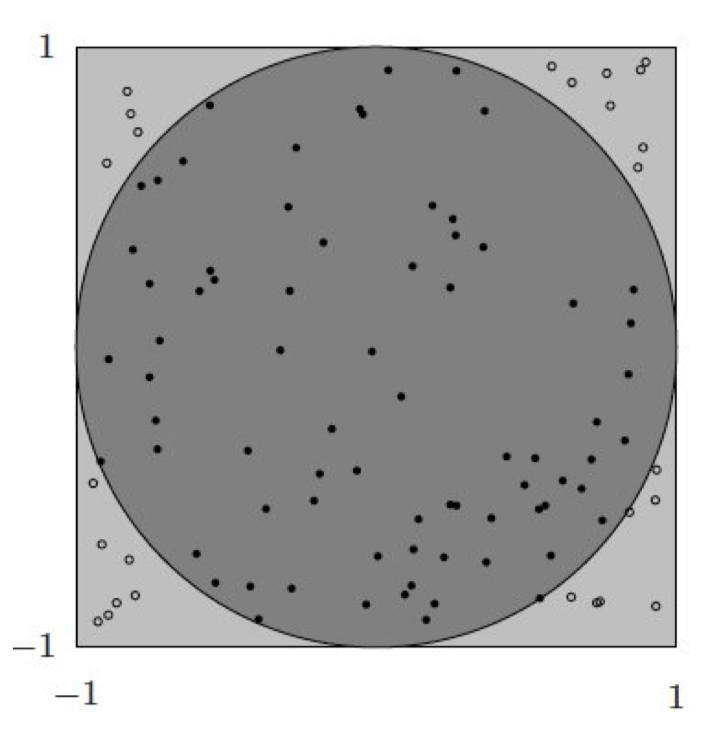
\includegraphics{images/circulo.png}
\caption{\label{fig:"sd"}}
\end{figure}

Sea \(P\) dicha probabilidad, por calculo:

\[P=\frac{\textrm{área del círculo}}{\textrm{área del cuadrado}}=\frac{\int_{-1}^1dx\int_{-\sqrt{1-x^2}}^{\sqrt{1-x^2}}dy}{\int_{-1}^1dx\int_{-1}^1dy}=\frac{2\int_{-1}^1\sqrt{1-x^2}dx}{2.2}=\frac{\pi}{4}\]

Es decir \(\pi=4P\). Ahora notemos lo siguiente:

\begin{itemize}
\item
  Gracias a los métodos de integración de cálculo podemos relacionar rapidamente la probabilidad con \(\pi\)
\item
  Con un ordenador podemos generar números o pares de números pseudo aleatorios \((x,y)\) entre 0 y 1.
\item
  Entre mayor número de simulaciones realicemos mayor sera nuestra aproximación a \(\pi\)
\end{itemize}

Para finalizar el ejemplo debemos encontrar la frcuencia de puntos que caen dentro de la circunferencia para aproximar \(P\) de una manera correcta, así despues de 1000 simulaciones \(\pi\approx 3,158733\).

\hypertarget{numeros-pseudoaleatorios}{%
\subsubsection{Números pseudoaleatorios}\label{numeros-pseudoaleatorios}}

Hemos visto que el método de MonteCarlo es un proceso estocástico númerico que nos permite resolver problemas de aproximación. Para ello se requiere muestrar variables aleatorias según una ley de distribución de probabilidad, por lo tanto es vital que nuestro método de muestreo sea efectivo, por lo tanto presentamos el siguiente test de calidad de números pseudoaleatorios.

\begin{itemize}
\item
  Equidistribución: los números pseudoaleatorios deben repartirse por igual, como correspondería a una verdadera distribución uniforme
\item
  Largo periodo: todos los métodos de generación de números pseudoaleatorios tienen un periodo en el cual la secuencia de números se vuelve a repetir, por lo tanto, el periodo debe ser largo para no agotar la sequencia en un cálculo concreto.
\item
  Repetibilidad: a veces se necesita repetir un cálculo con exactamente los mismos números pseudoaleatorios. Así que conviene que el generador permita almacenar su estado
\item
  Largas subsecuencias disjuntas: Si la simulación es muy extensa resulta conveniente subdividirla en otras más pequeñas, para lo que es importante que sean estadísticamente independientes y así se puedan recombinar sin introducir correlaciones.
\end{itemize}

Portabilidad: La rutina debe generar exactamente la misma secuencia de números no solamente por distintos lenguajes de programación sino también en distintas máquinas.

Eficiencia: La generación de cada número debe consumir muy poco tiempo.

Ahora para comprobar la eficiencia del método de generación de números pseudo aleatorios existen test estadísticos para comprobar su bondad, los mas usados son:

\begin{itemize}
\item
  Test de frecuencia: Sirve para comprobar la equidistribución de \(N\) valores generados.Se divide el intervalo \([0,1]\) en \(k\) sub intervalos. Uno esperaría encontrar \(N/k\) valores en cada sub intervalo. Sea \(N_j\) la cantidad de valores encontrados en el intervalo \(j\)-ésimo. Entonces la siguiente \(\chi^2\) permite hallar la probabilidad de que la distribución generada sea compatible con una verdadera distribución aleatoria uniforme,\[\chi^2=\frac{k}{N}\sum_{j=1}^k\bigg{(}N_j-\frac{N}{k}\bigg{)}^2\] que se comportara asintóticamente como una \(\chi^2(k-1)\)
\item
  Test de la serie: Sirve para comprobar la independencia entre sucesivos numeros en una secuencia. Es una generalización del test anterior. Dividinos el intervalo \([0,1]\) en \(r\) sub intervalos y miramos ternas de \(s\geq2\) puntos \(x_n=(x_n,x_{n+1},...,x_{n+s-1})\) consecutivamente generados. Cada una de las \(N\) ternas \(x_n\) generadas caerá dentro de uno de los \(r^s\) bines en los que se divide este espacio \(s\) dimensional. Si llamamos \(N_{j_1,j_2,...j_s}\) con \(j_i\in\{1,2,3,...,r\}\), el número de valores que caen en el bin \((j_1,j_2,...,j_s)\), la siguiente \(\chi^2\) nos permita hallar la probabilidad de que la distribución generada sea uniforme, \[\chi^2=\frac{r^s}{N}\sum_{\{j_1,j_2,...j_s\}}\bigg{(}N_{j_1,j_2,...j_s}-\frac{N}{r^s}\bigg{)}\] Se comportara asintóticamente como una \(\chi^2(r^2-1)\)
\end{itemize}

\hypertarget{aplicando-simulacion-de-montecarlo-para-hallar-la-distribucion-de-perdidas-de-una-cartera.}{%
\subsubsection{Aplicando simulación de MonteCarlo para hallar la distribución de pérdidas de una cartera.}\label{aplicando-simulacion-de-montecarlo-para-hallar-la-distribucion-de-perdidas-de-una-cartera.}}

Ahora una vez se pretenda usar un método algorítmico de generación de números aleatorios, se usa este metódo para generar eventos probabilísticos en los cuales se consideren todos los posibles eventos de transición entre las distintas calificaciones. Cada evento se considera como una simulación de un evento particular, por cada simulación los créditos se encuentran en una calificación determinada por la probabilidad de transición respectiva, este calificación trae con si una pérdida esperada por crédito, asi por cada simulación se obtiene una pérdida.

Ahora si nuestra cartera de crédito posee 1000 créditos, y existen 5 calificaciones, en la sección vimos que existen \(5^{1000}\) posibles eventos, para imaginarnos esta cantidad basta saber que este número es mayor que un billón, por lo tanto debemos realizar un gran número de simulaciones para poder captar información verídica de la pérdida esperada. Una de las bondades de estimar la pérdida esperada de esta forma es que la distribución tenderá asintóticamente a una normal donde su media tenderá la pérdida esperada de la cartera.

\hypertarget{obtencion-de-las-metricas-de-riesgo.}{%
\subsubsection{Obtención de las métricas de riesgo.}\label{obtencion-de-las-metricas-de-riesgo.}}

Una ves realizadas las simulaciones y obtenida la aproximación de la distribución de pérdidas usando la aproximación normal es facil obtener las métricas de riesgo, pues estas ya están definidas para la distribución normal. Si la distribucion de pérdidas es como una normal de media \(\mu\) y desvianción estándar \(\sigma\) las métricas de riesgo son: \[\textrm{Pérdida esperada}=\mu\],\[VaR_{p}=\mu+\sigma\Phi^{-1}(p)\],\[TVaR_p=\mu+\sigma\frac{\phi[\Phi^{-1(p)}]}{1-p}\]
Donde \(\phi\) y \(\Phi\) representan la función de densidad de probabilidad y la función de probabilidad acumulada de una normal estándar.

\mainmatter

\hypertarget{manual-tecnico-de-la-aplicacion-vision-creditrisk}{%
\chapter{Manual técnico de la aplicación Vision CreditRisk}\label{manual-tecnico-de-la-aplicacion-vision-creditrisk}}

En el presente capítulo, presentaremos el manual técnico de la aplicación Vision CreditRisk, el cual utiliza las nociones teóricas vistas anteriormente para lograr de una forma agradable y de facíl entendimiento permtir que el usuario encargado del área de crédito de su institución maneje de forma precisa y adecuada las métricas de riesgo.

\hypertarget{presentacion-de-la-aplicacion.}{%
\section{Presentación de la aplicación.}\label{presentacion-de-la-aplicacion.}}

La aplicación esta compuesta de ocho secciones, la primera una sección donde se cargan los datos que necesitará la aplicación, la segunda correspondiente a la sección \textbf{Scoring y Rating}, la tercera sección correspondiente a la \textbf{Pérdida por Incumplimiento}, la cuarta correspondiente a la \textbf{Matriz de transición}, la quinta correspondiente a la metodología \textbf{CreditRisk+}, la sexta a la metología \textbf{CreditMetrics}, la septima correspondiente al \textbf{BackTesting} y la octava a correspondiente a los \textbf{Indicadores contables}.

\begin{figure}
\centering
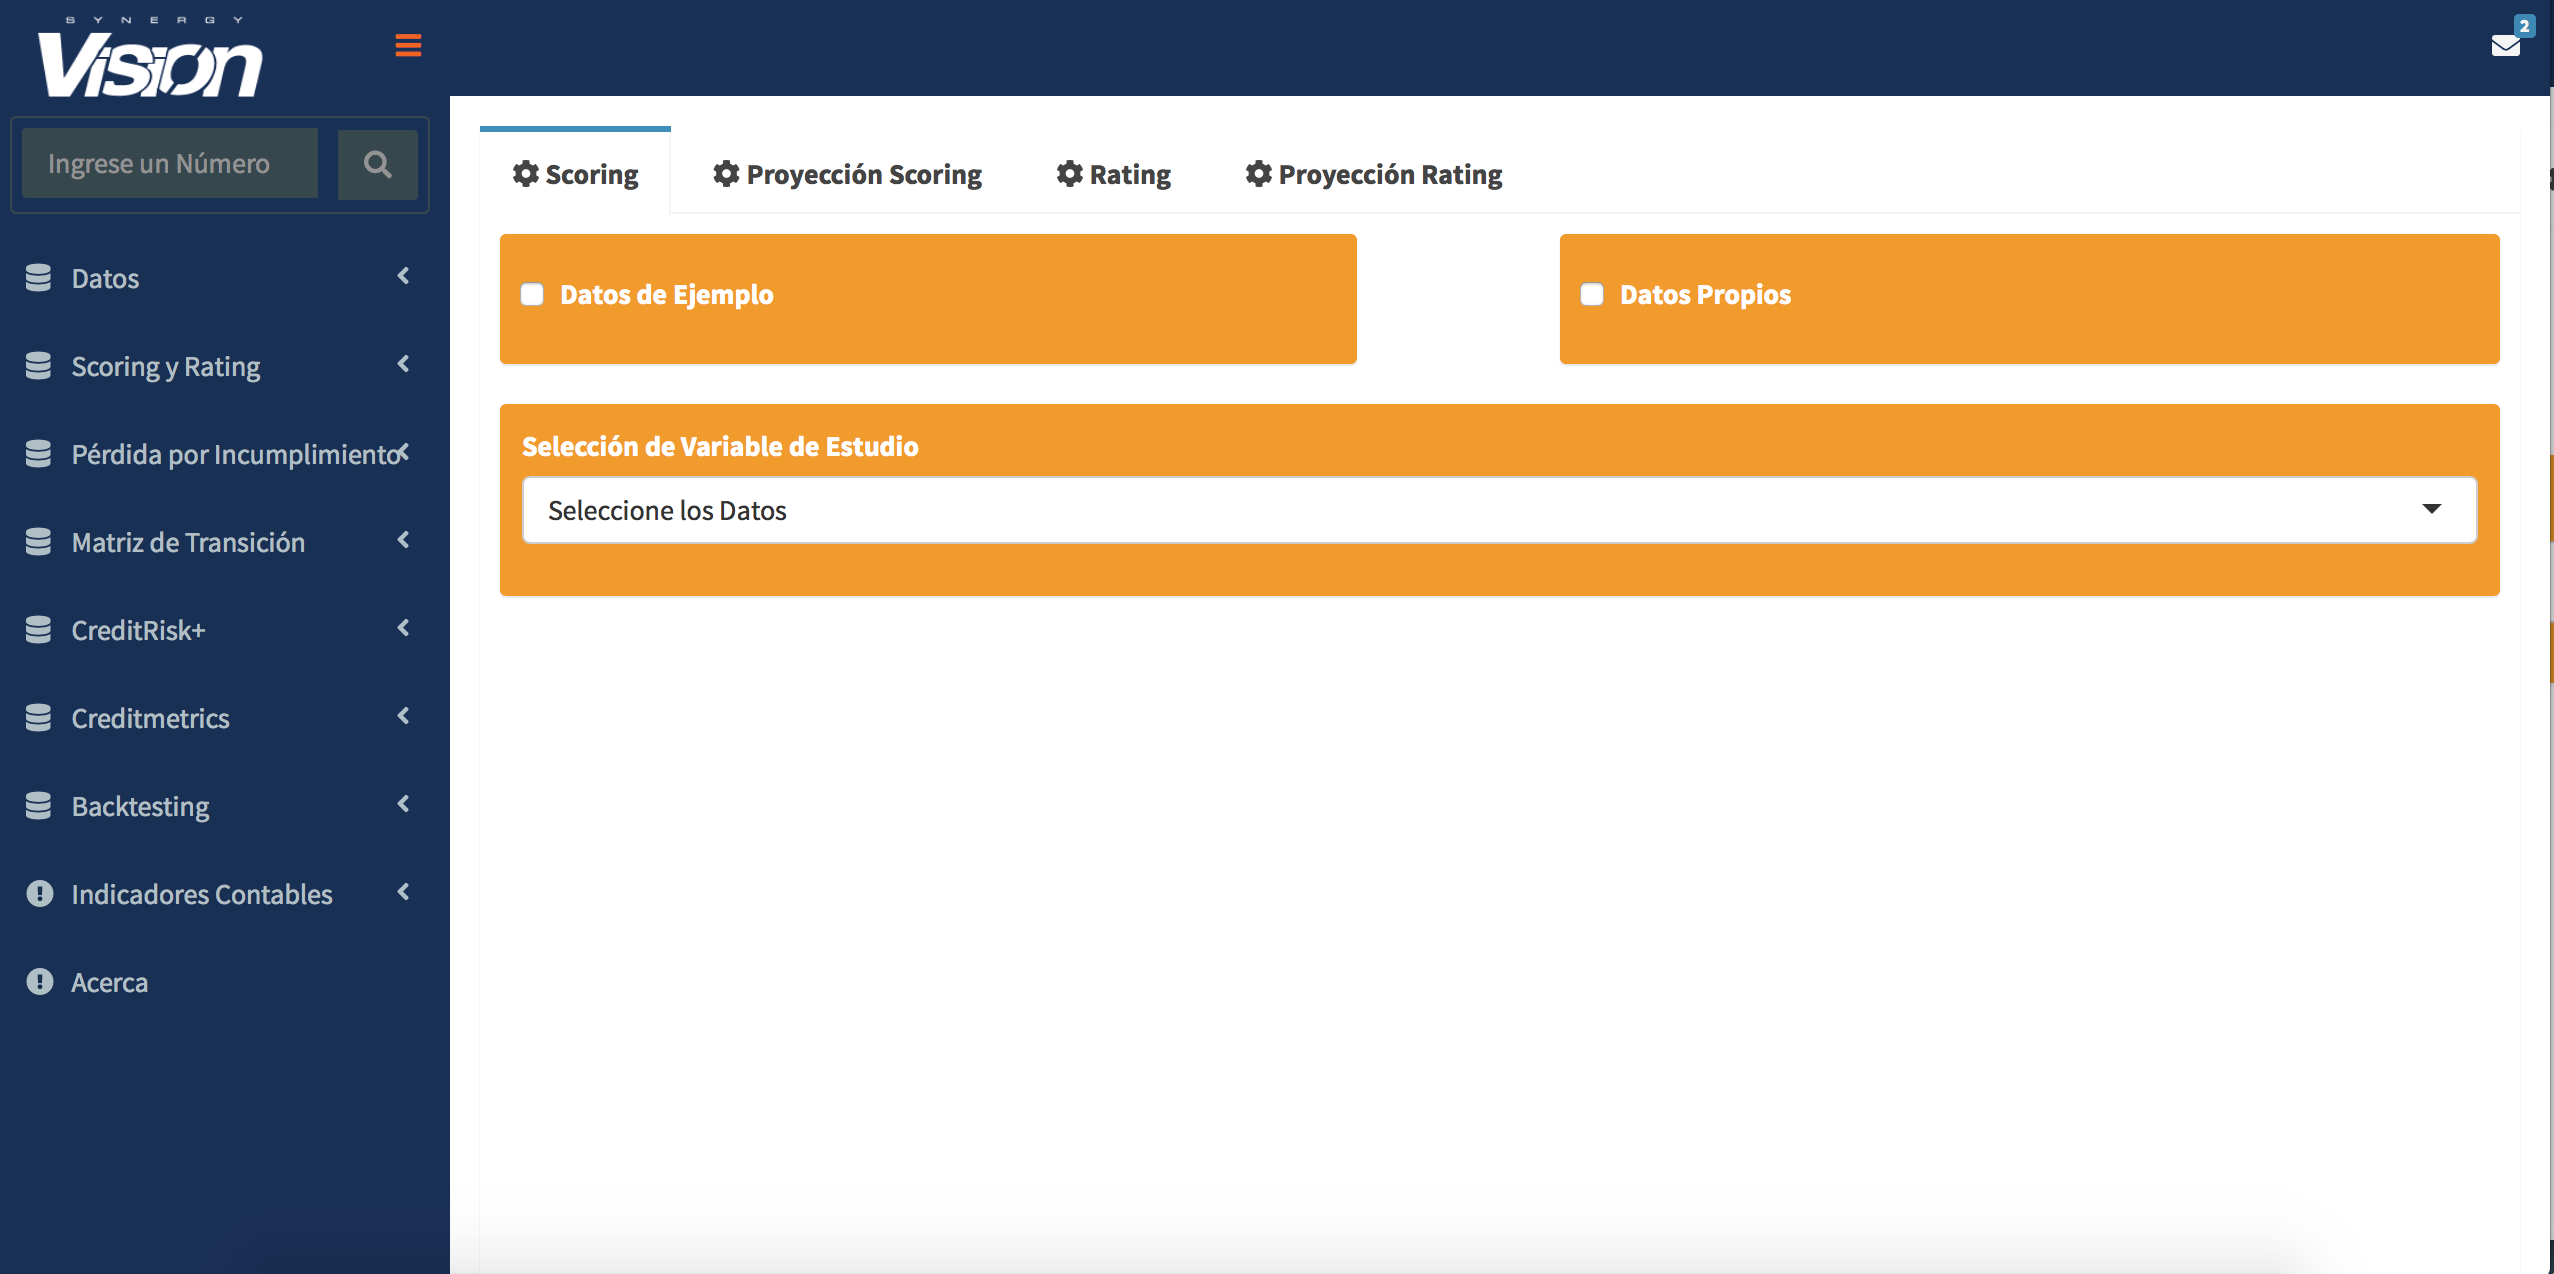
\includegraphics{images/1.png}
\caption{\label{fig:"sd"}}
\end{figure}

\hypertarget{primera-seccion-datos}{%
\section{Primera sección: Datos}\label{primera-seccion-datos}}

En esta sección se cargan los datos de las diferentes metodologías

\begin{figure}
\centering
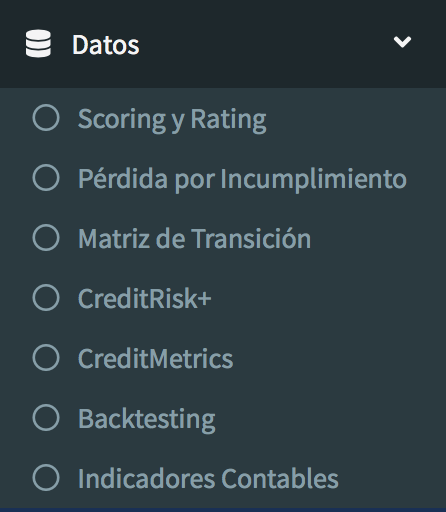
\includegraphics{images/2.png}
\caption{\label{fig:"sd"}}
\end{figure}

\hypertarget{scoring-y-rating}{%
\subsection{Scoring y Rating}\label{scoring-y-rating}}

En esta sección se cargan los datos con los cuales serán construidos el \textbf{Score y Rating} de crédito.

\hypertarget{scoring}{%
\subsubsection{Scoring}\label{scoring}}

En esta sección se tendrá dos opciones, la primera será de datos de ejemplo, la cual se muestra a continuación

\begin{figure}
\centering
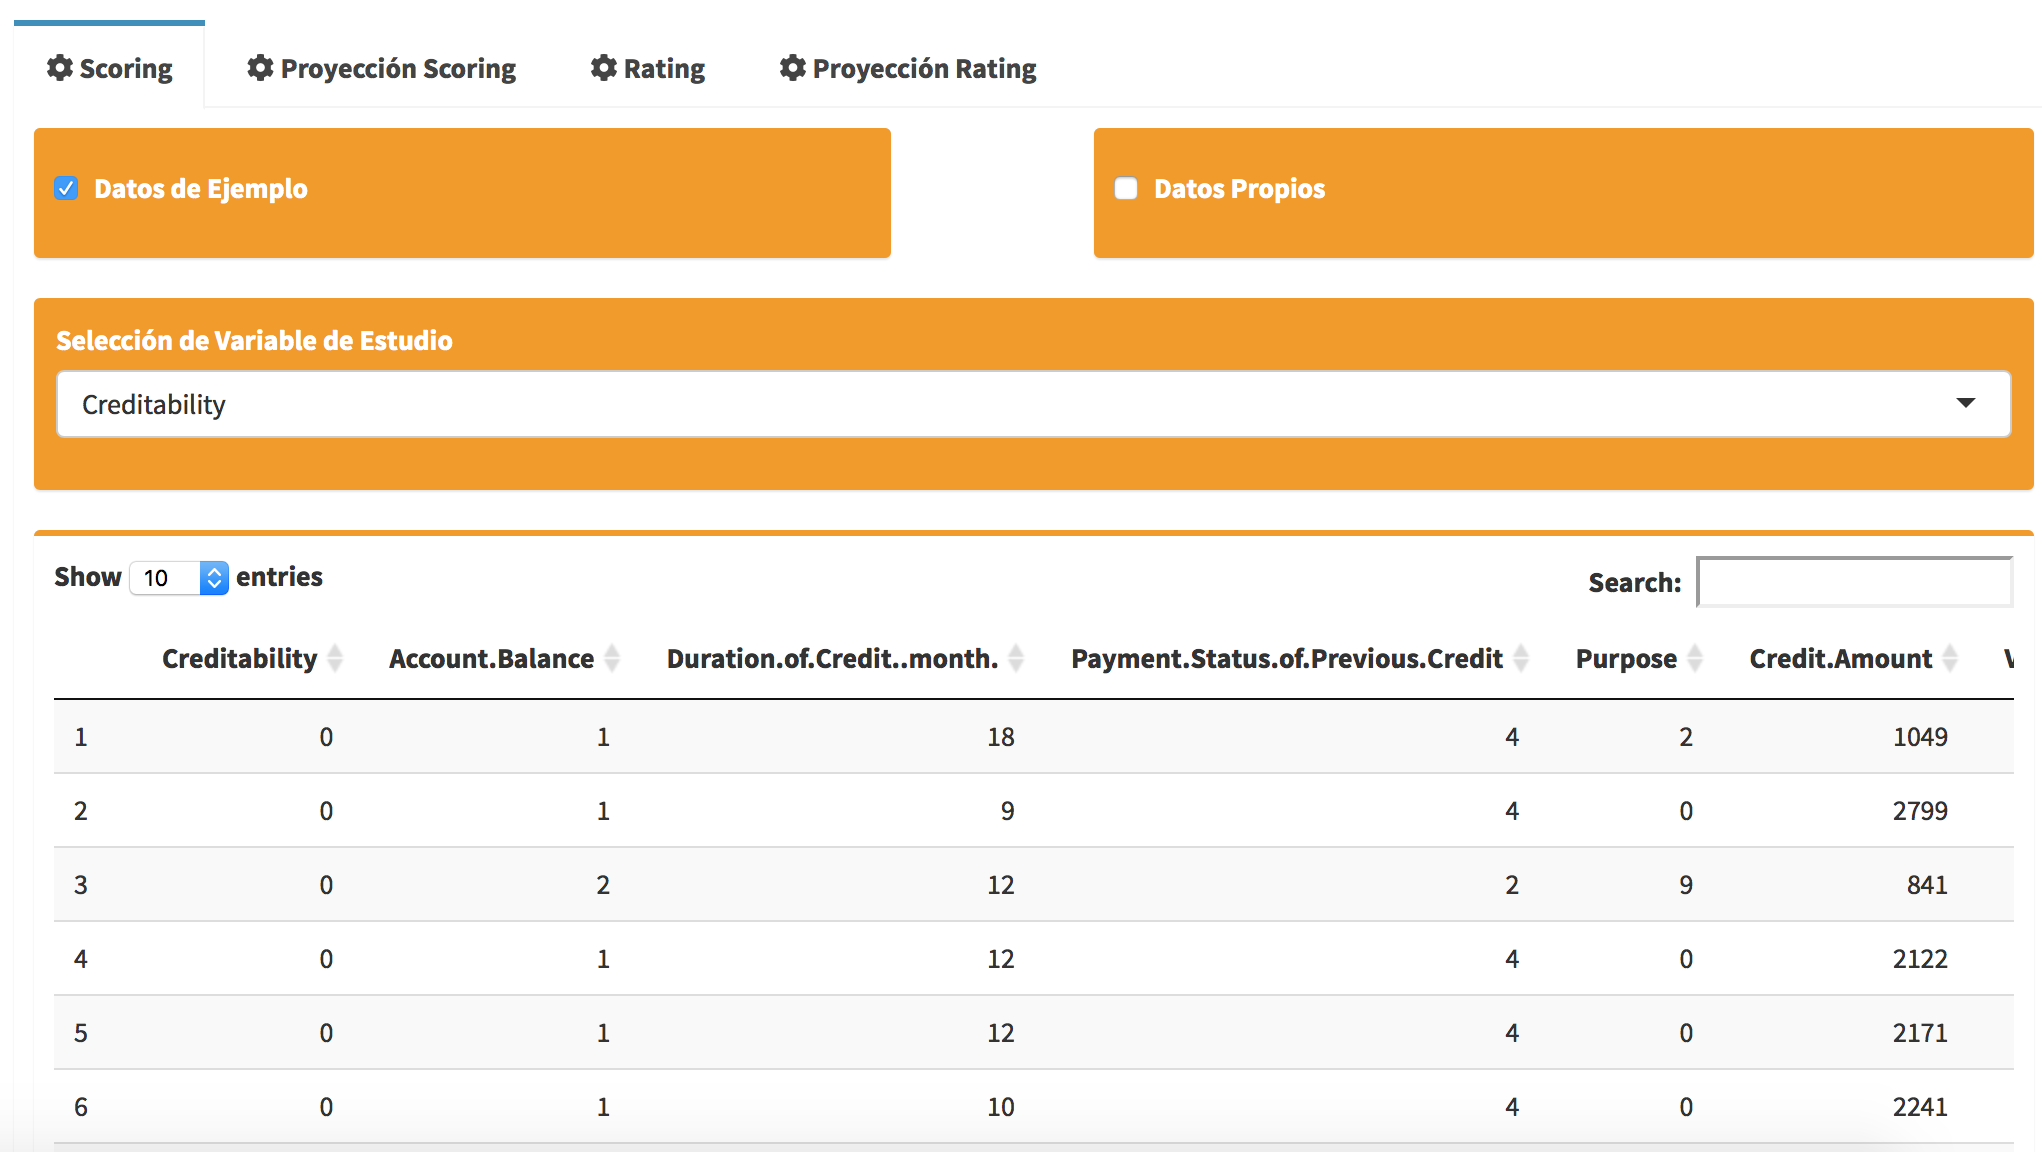
\includegraphics{images/4.png}
\caption{\label{fig:"sd"}}
\end{figure}

La segunda \emph{Datos Propios} la cual debemos cargar los datos de la aplicación.

\begin{figure}
\centering
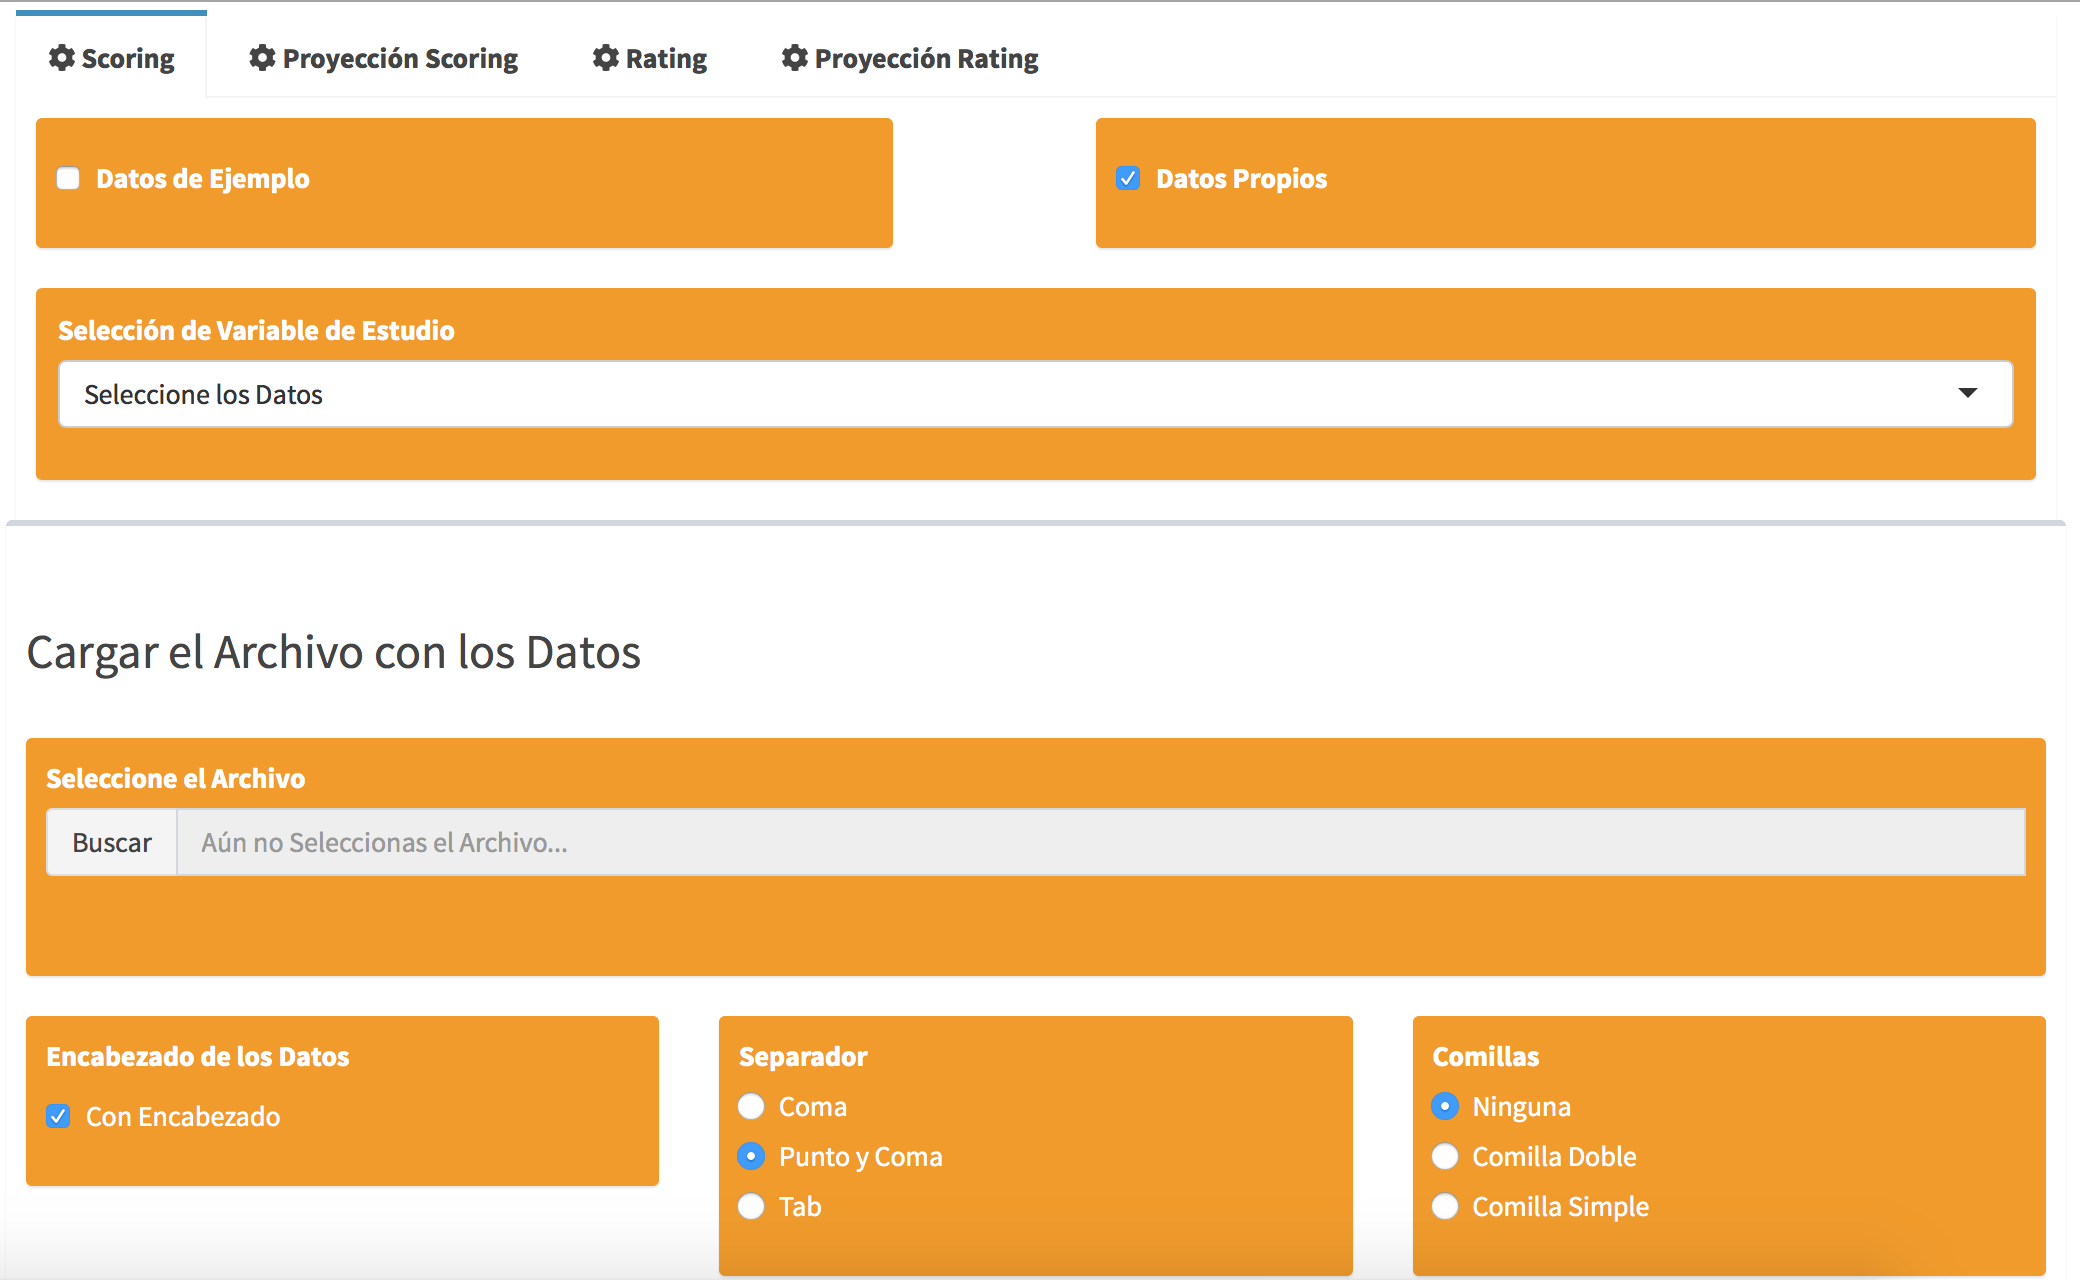
\includegraphics{images/5.png}
\caption{\label{fig:"sd"}}
\end{figure}

\hypertarget{proyeccion-scoring}{%
\subsubsection{Proyección Scoring}\label{proyeccion-scoring}}

En Proyección Scoring cargamos datos para hacer predicciones de nuevos clientes.

\begin{figure}
\centering
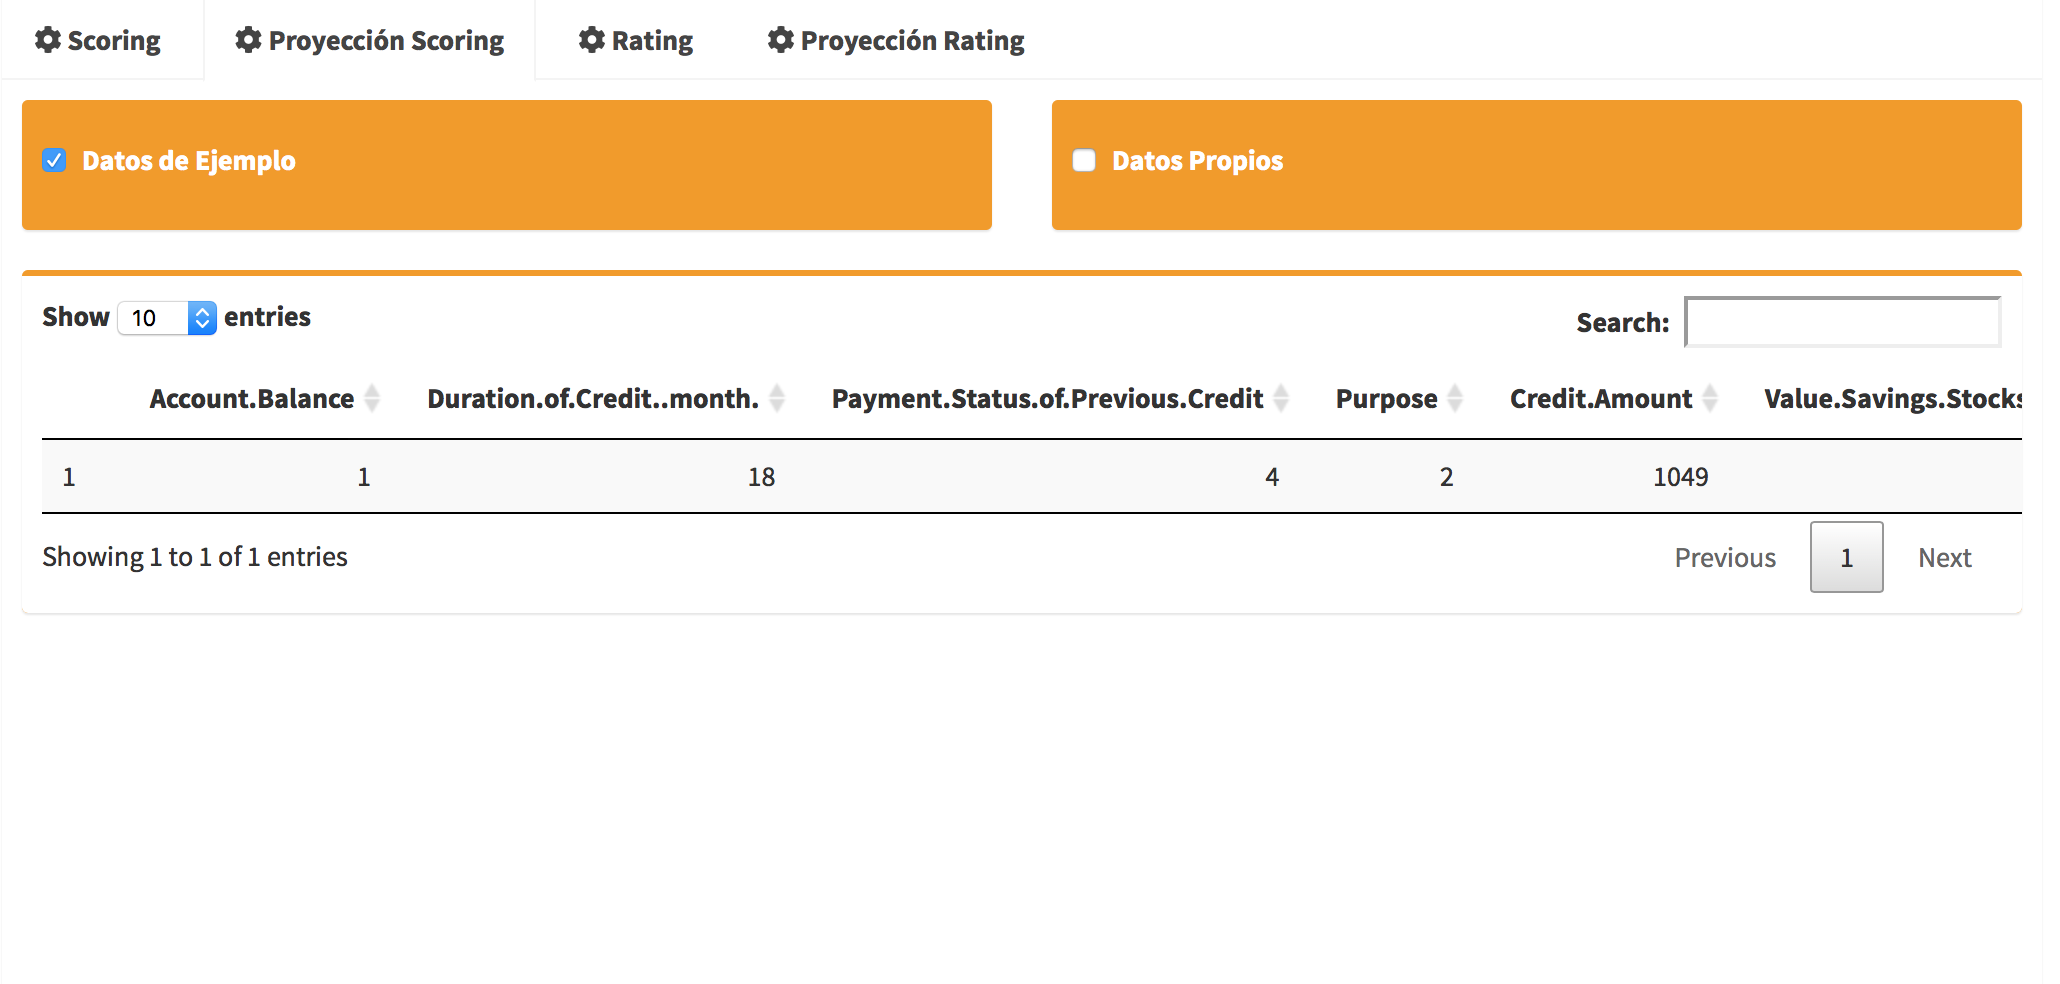
\includegraphics{images/6.png}
\caption{\label{fig:"sd"}}
\end{figure}

\hypertarget{rating}{%
\subsubsection{Rating}\label{rating}}

En Rating cargamos los datos como se muestra a continuación

\begin{figure}
\centering
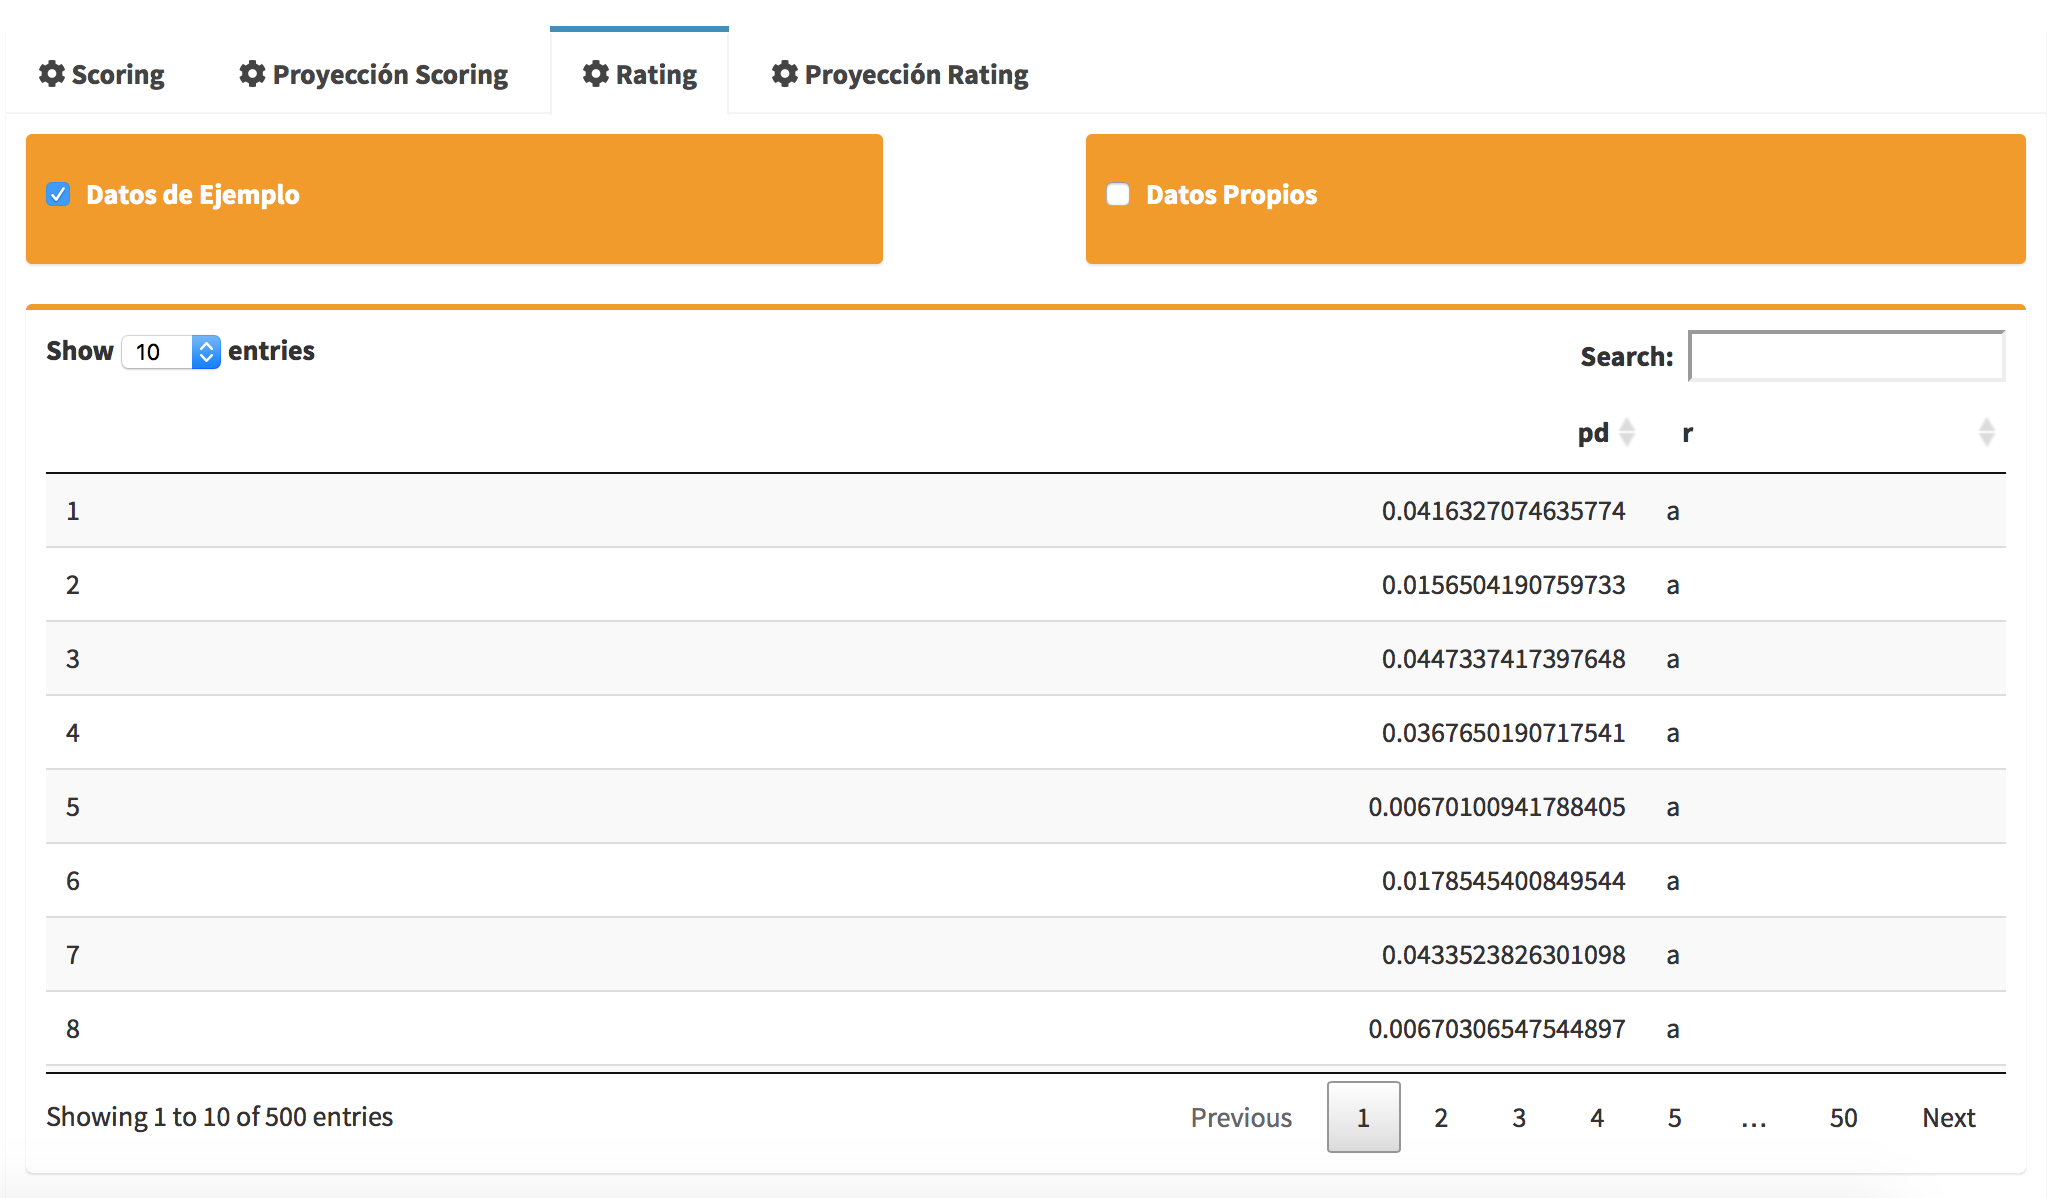
\includegraphics{images/7.png}
\caption{\label{fig:"sd"}}
\end{figure}

\hypertarget{proyeccion-rating}{%
\subsubsection{Proyección Rating}\label{proyeccion-rating}}

En \emph{proyrección rating} tenemos dos opciones, en la primera usamos datos provenientes del Score o datos propios.

\begin{figure}
\centering
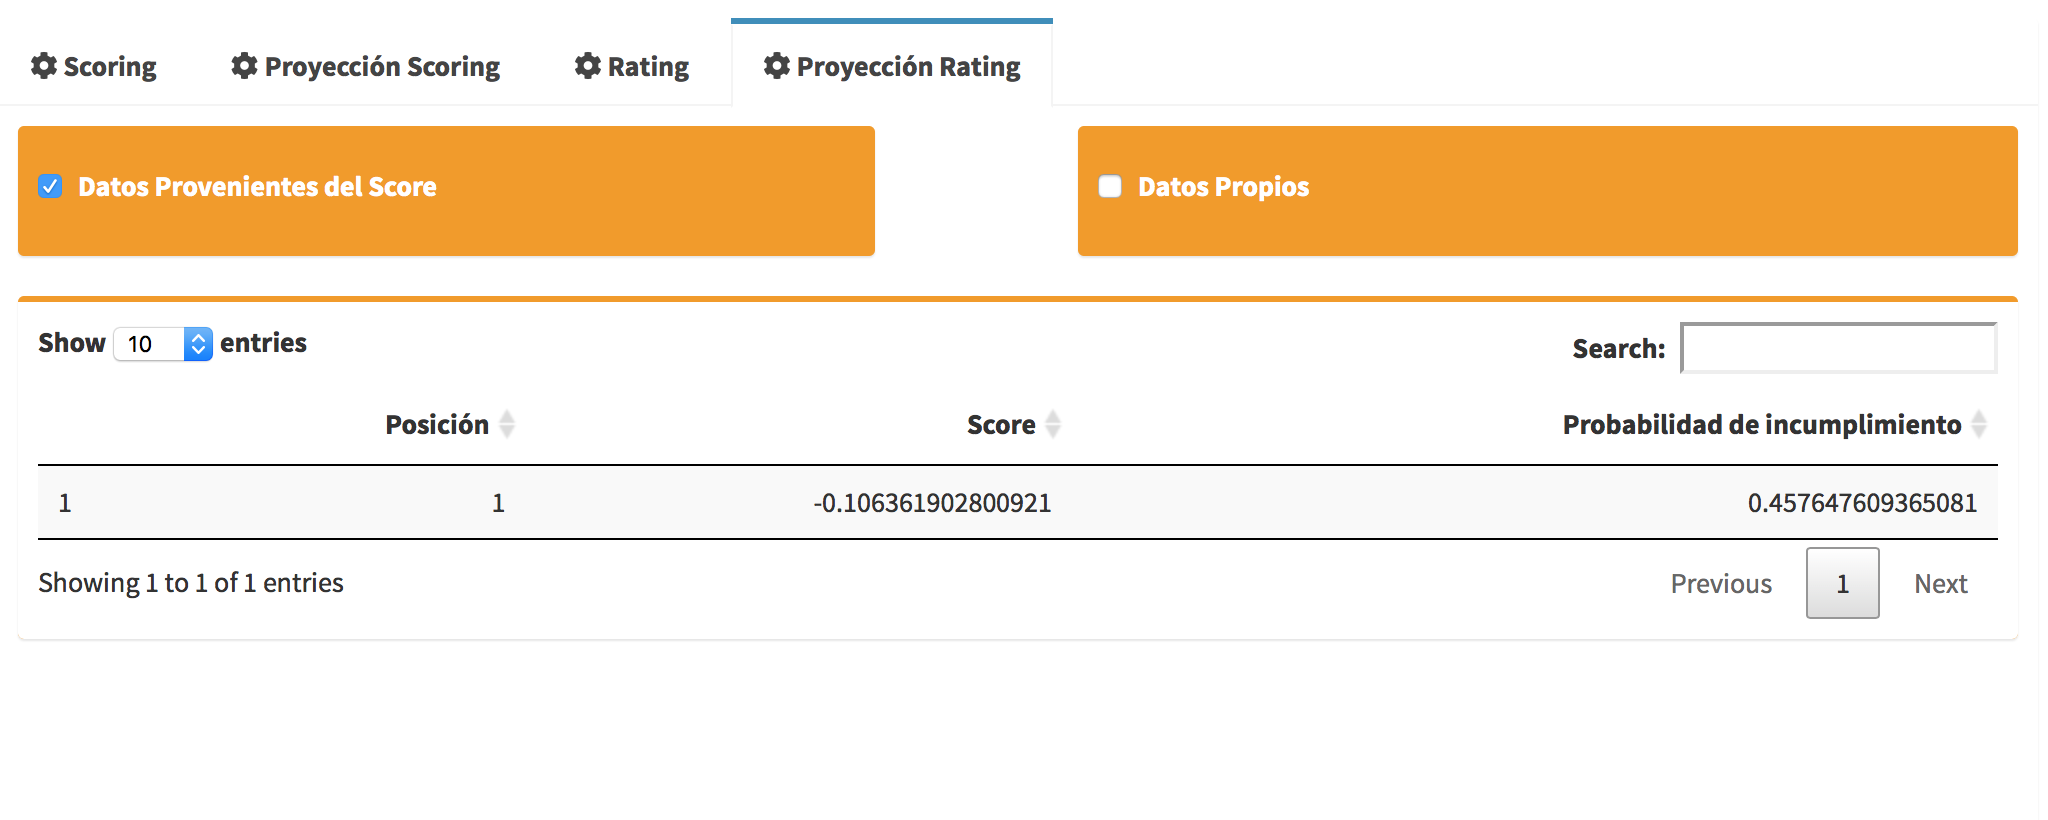
\includegraphics{images/8.png}
\caption{\label{fig:"sd"}}
\end{figure}

\hypertarget{perdida-por-incumplimiento}{%
\subsection{Pérdida por Incumplimiento}\label{perdida-por-incumplimiento}}

En esta sección cargaremos los datos para estimar las pérdida esperada de los clientes.

\hypertarget{perdida-por-clientes}{%
\subsubsection{Pérdida por clientes}\label{perdida-por-clientes}}

Se cargan los datos de pérdidas históricas por clientes.

\begin{figure}
\centering
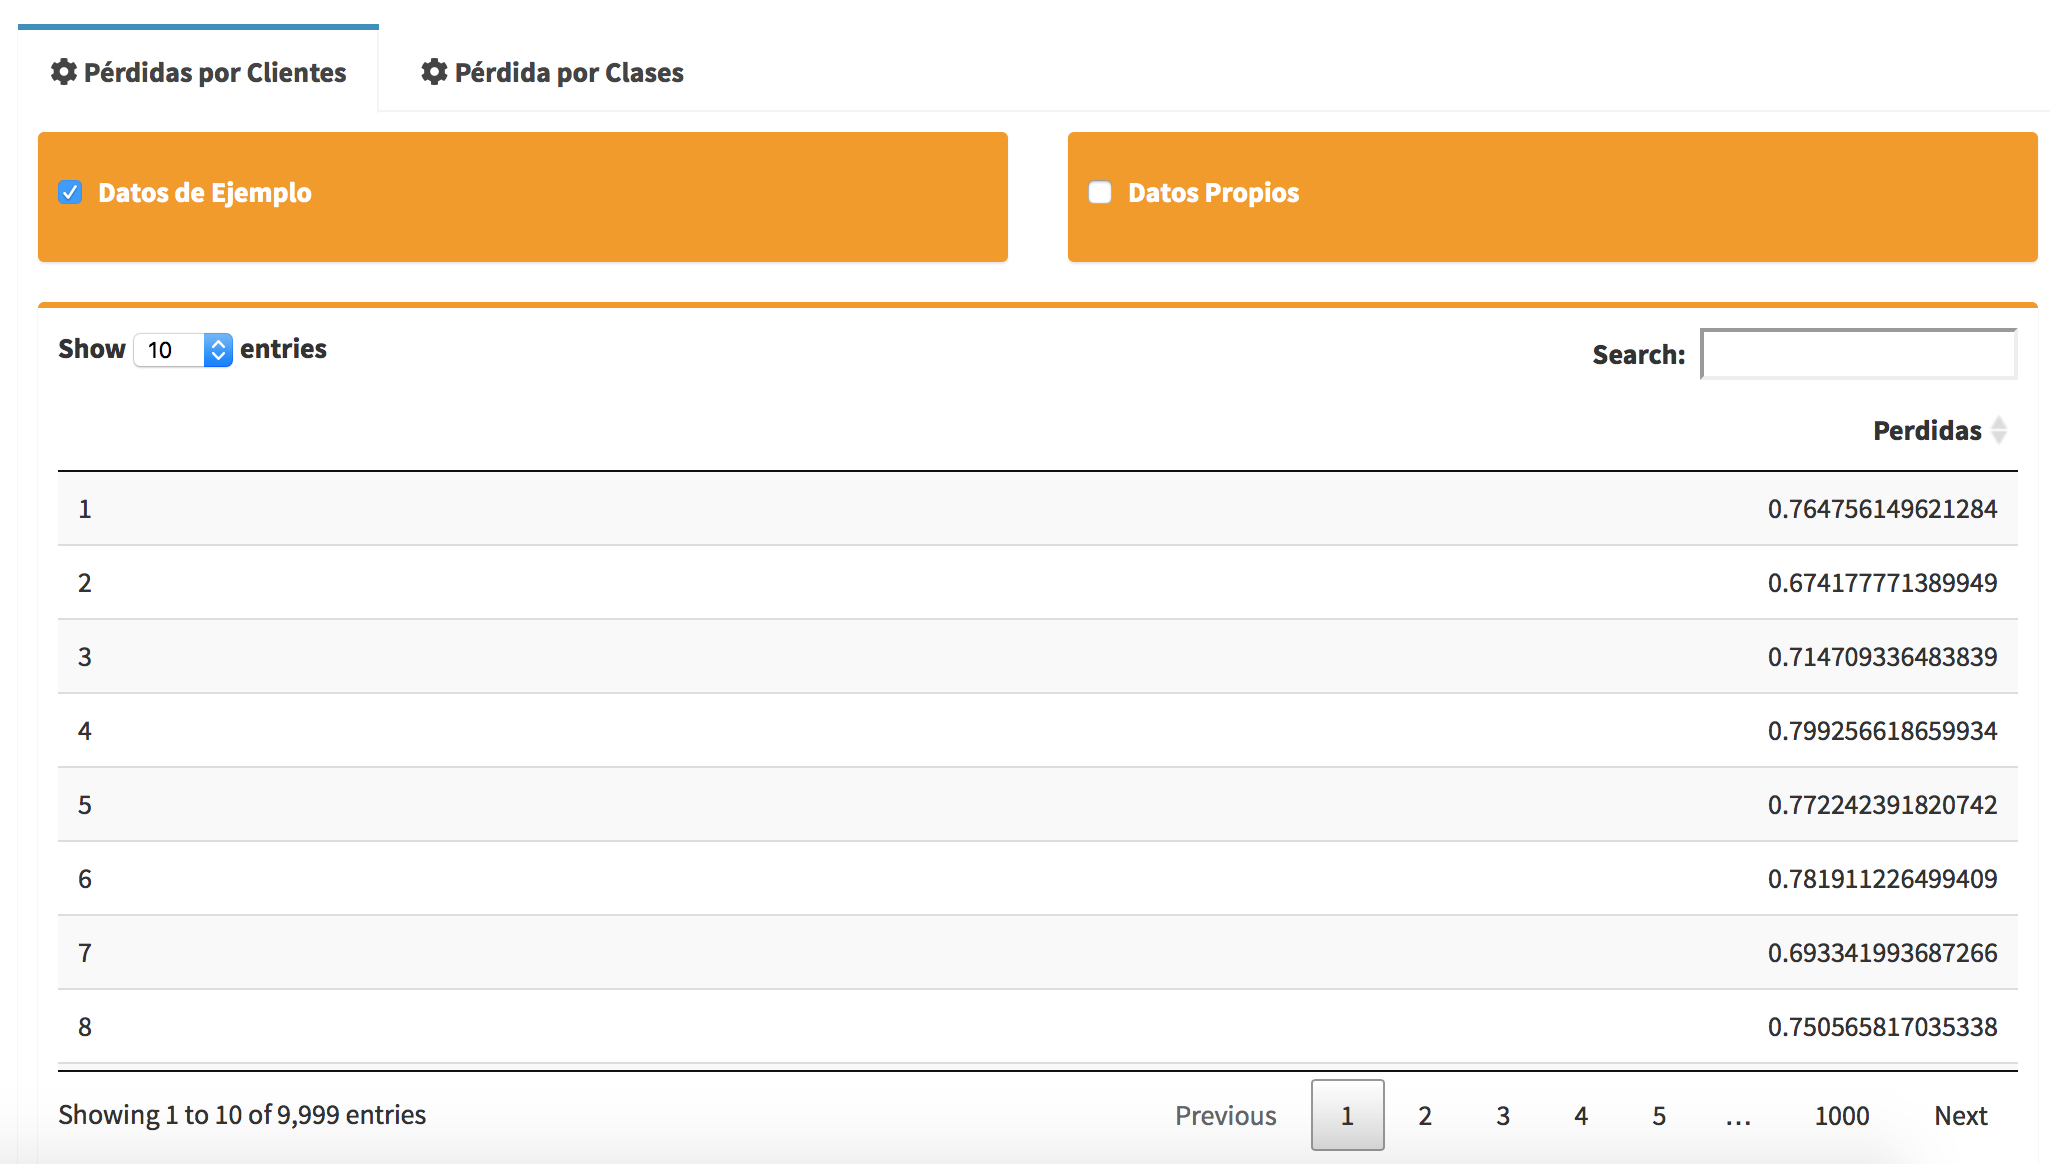
\includegraphics{images/9.png}
\caption{\label{fig:"sd"}}
\end{figure}

\hypertarget{perdida-por-clase}{%
\subsubsection{Pérdida por clase}\label{perdida-por-clase}}

Se cargan los datos de pérdidas históricas por clientes y sus categorías crediticias.

\begin{figure}
\centering
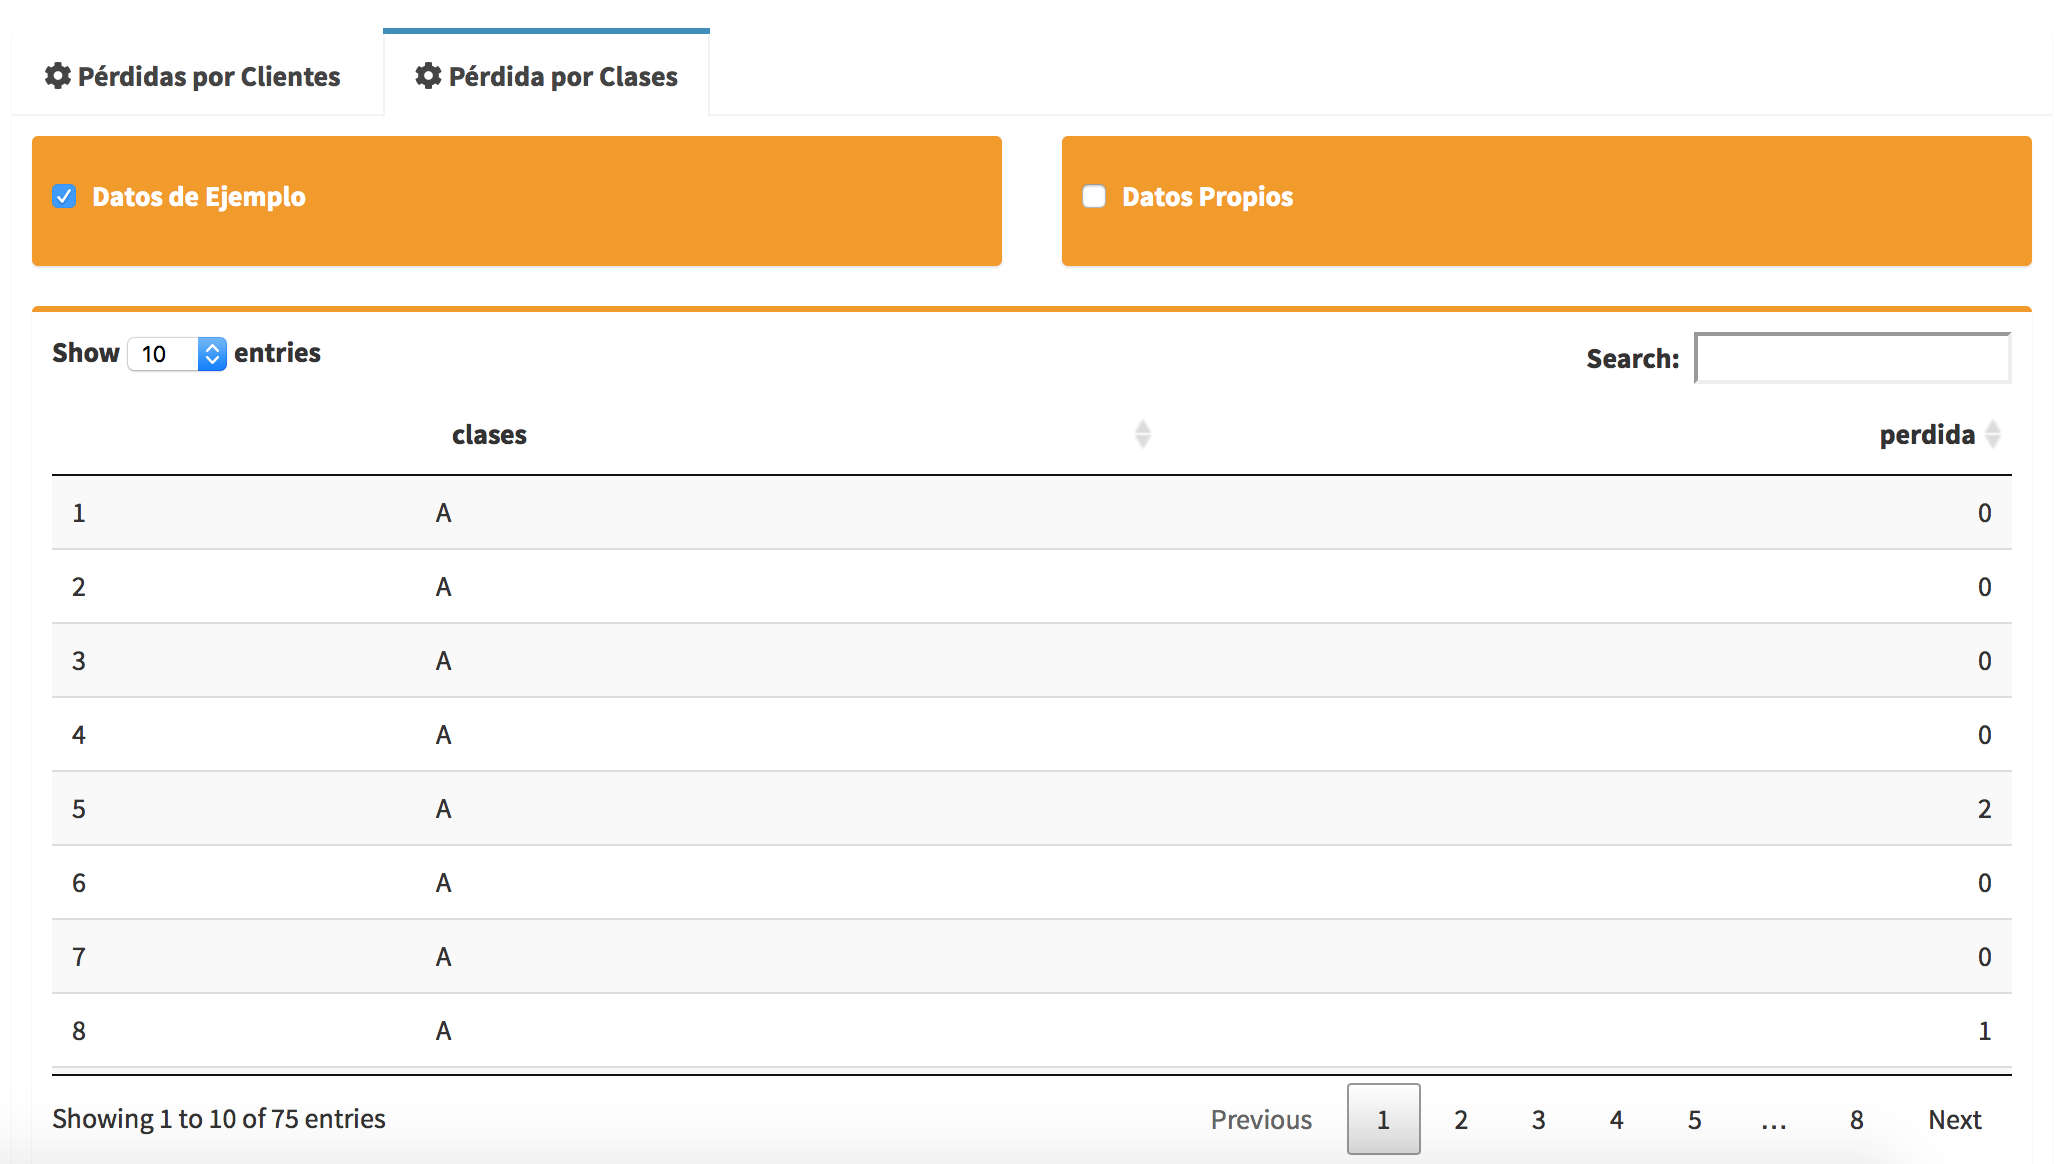
\includegraphics{images/10.png}
\caption{\label{fig:"sd"}}
\end{figure}

\hypertarget{matriz-de-transicion-1}{%
\subsection{Matriz de transición}\label{matriz-de-transicion-1}}

En esta sección solo tendremos una pestaña en la cual se cargarán los datos de las transiciones históricas entre categorías.

\begin{figure}
\centering
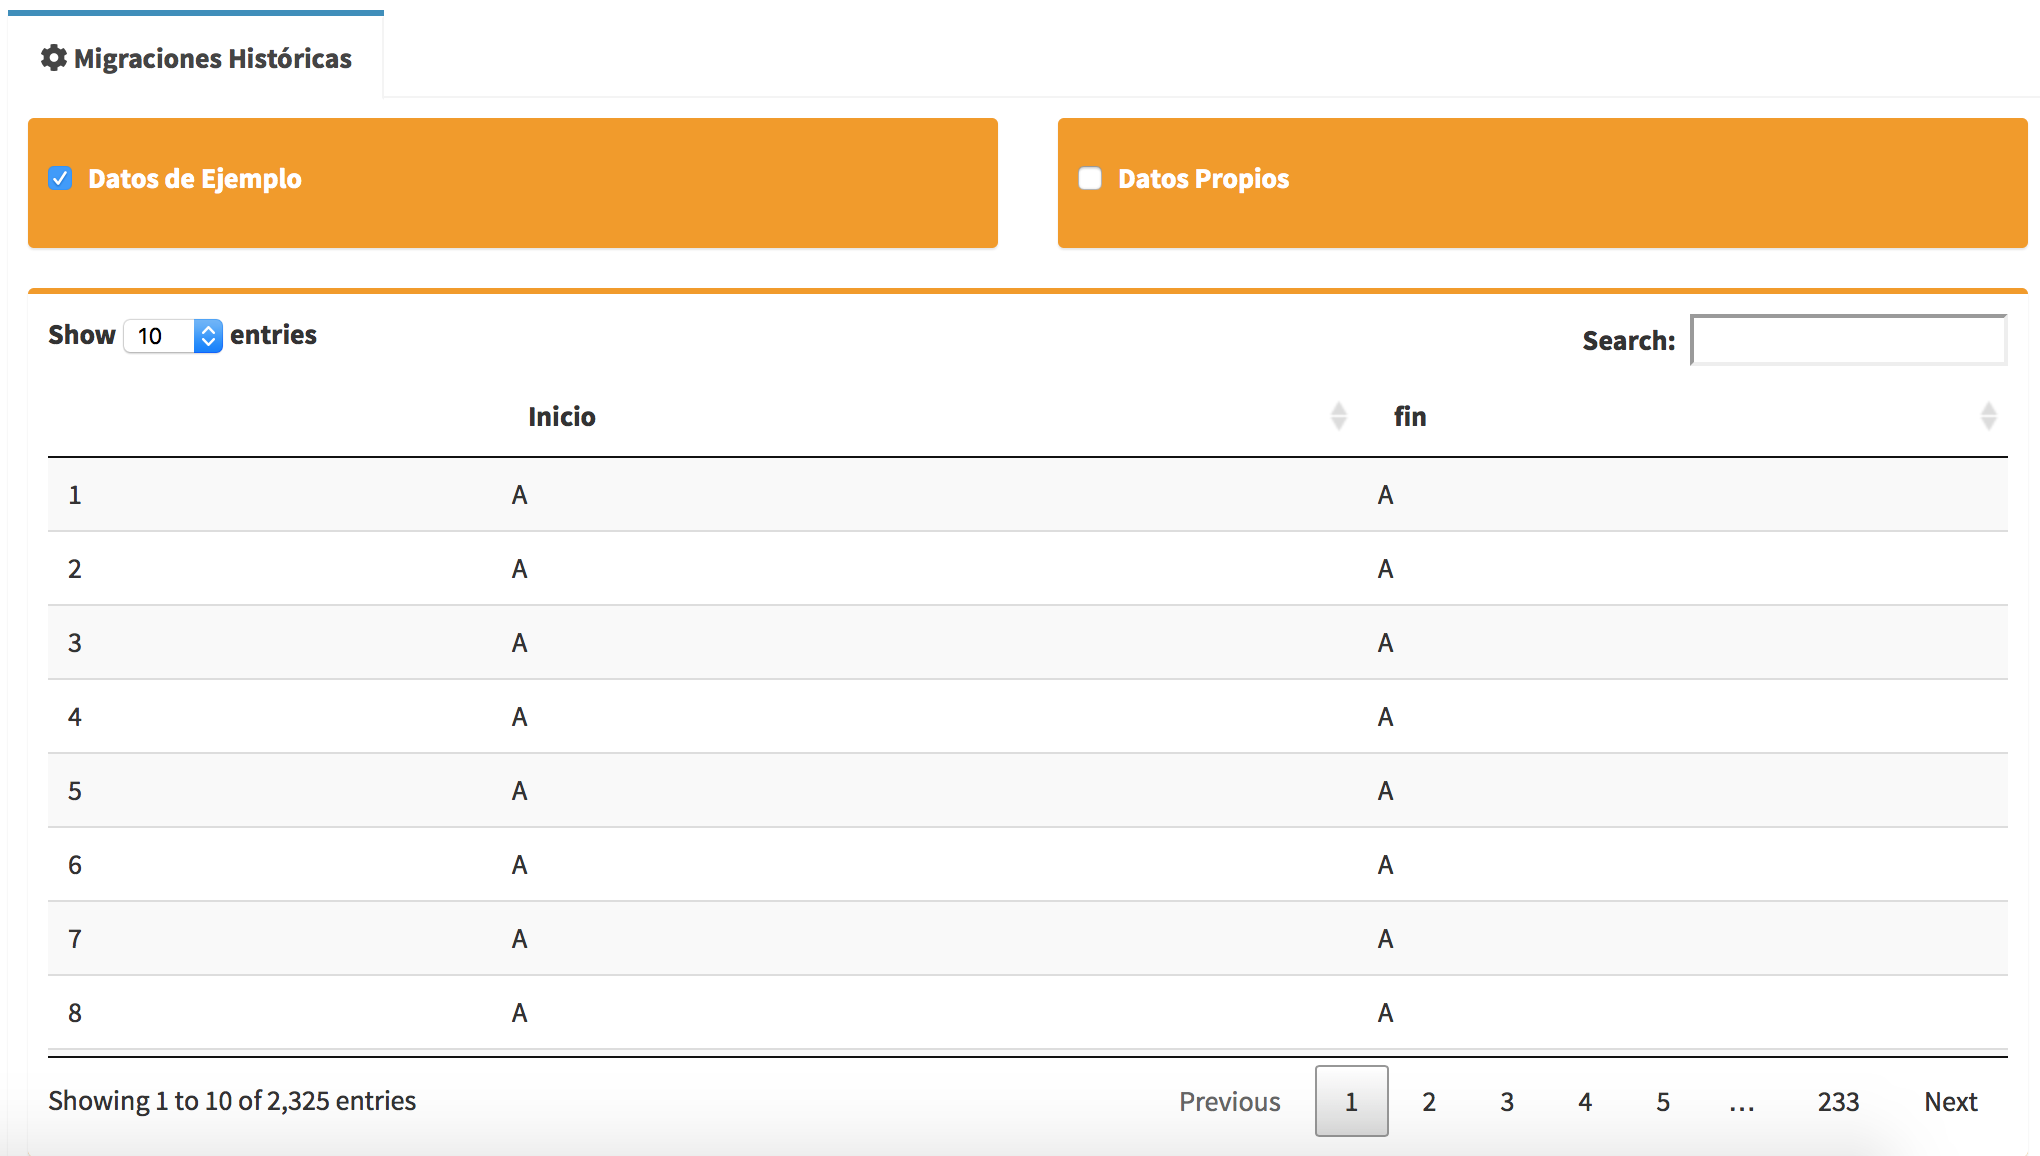
\includegraphics{images/11.png}
\caption{\label{fig:"sd"}}
\end{figure}

\hypertarget{creditrisk-1}{%
\subsection{CreditRisk+}\label{creditrisk-1}}

En esta sección cargaremos los datos de la primera metodología de riesgo de crédito.

\hypertarget{exposicion}{%
\subsubsection{Exposición}\label{exposicion}}

Primero cargamos los datos correspondientes a la exposición crediticia de cada cliente.

\begin{figure}
\centering
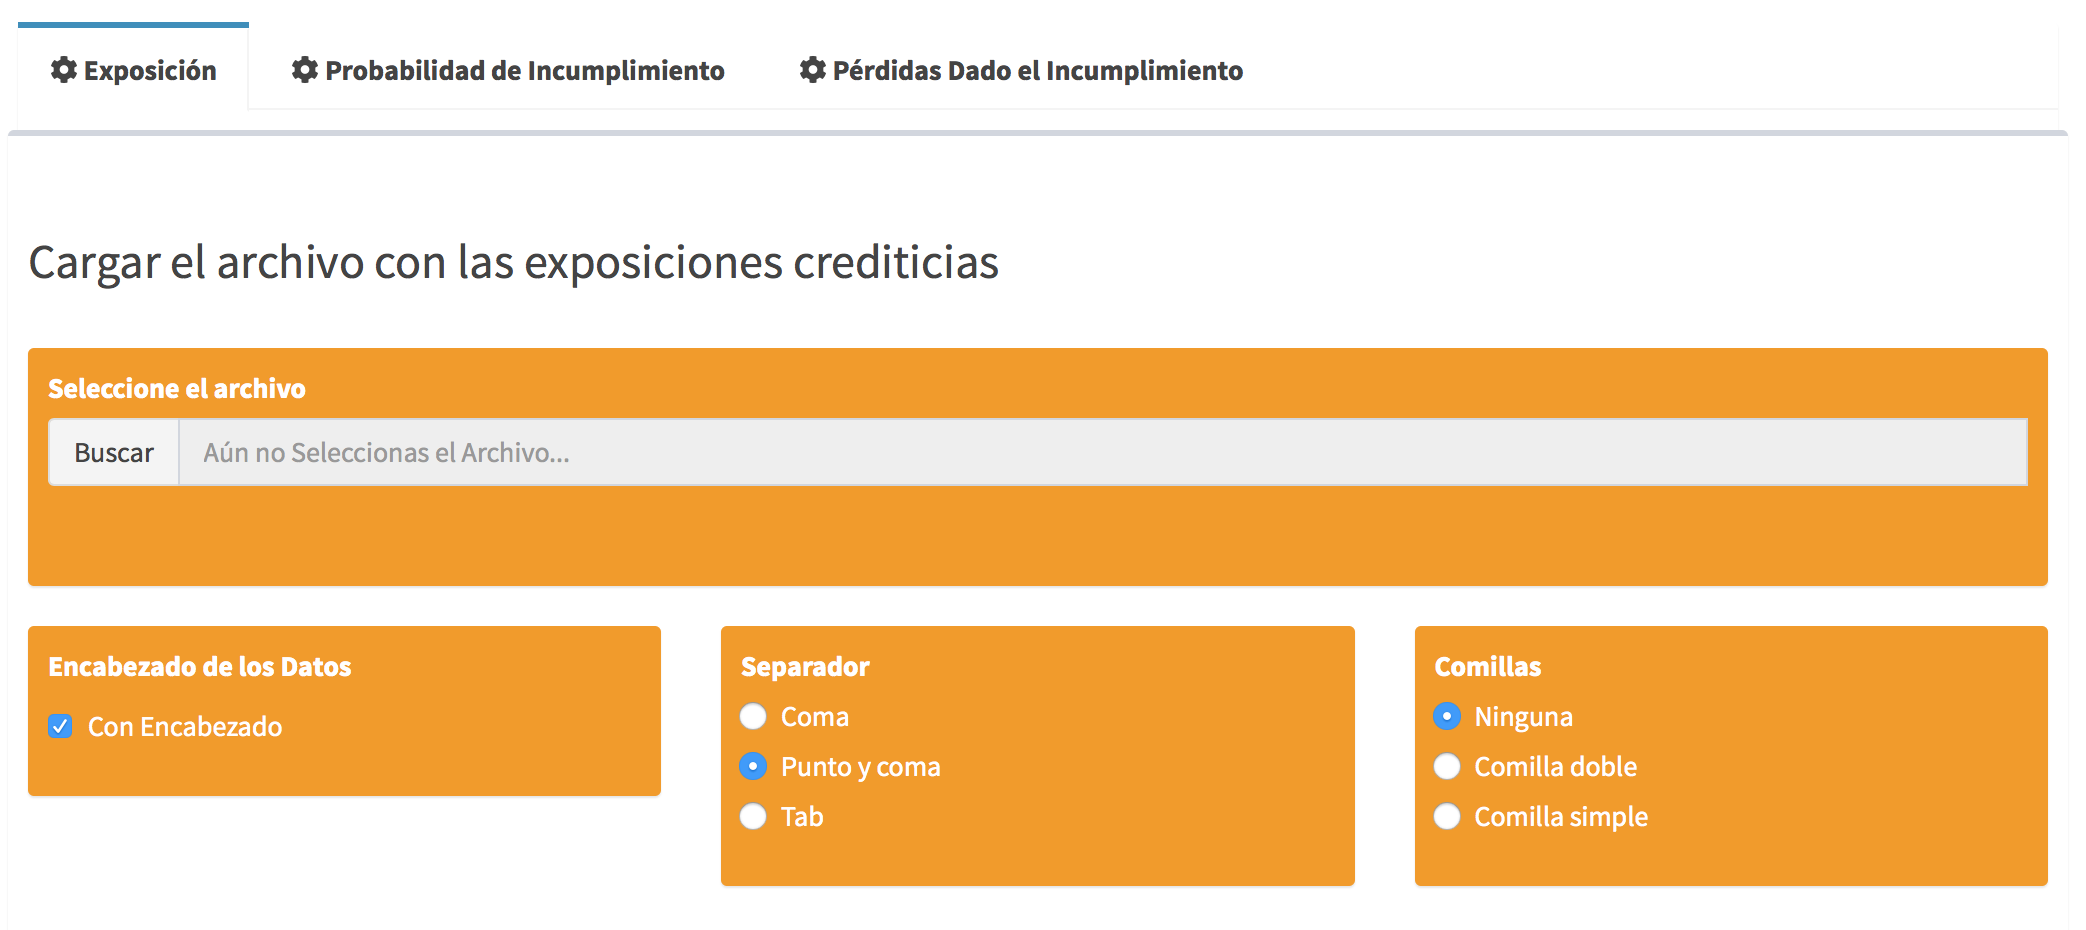
\includegraphics{images/14.png}
\caption{\label{fig:"sd"}}
\end{figure}

\hypertarget{probabilidad-de-incumplimiento}{%
\subsubsection{Probabilidad de incumplimiento}\label{probabilidad-de-incumplimiento}}

Se cargan las probabilidades de incumplimiento de cada cliente, en este caso podemos seleccionar un conjunto de datos propios o los provenientes de la sección Score

\begin{figure}
\centering
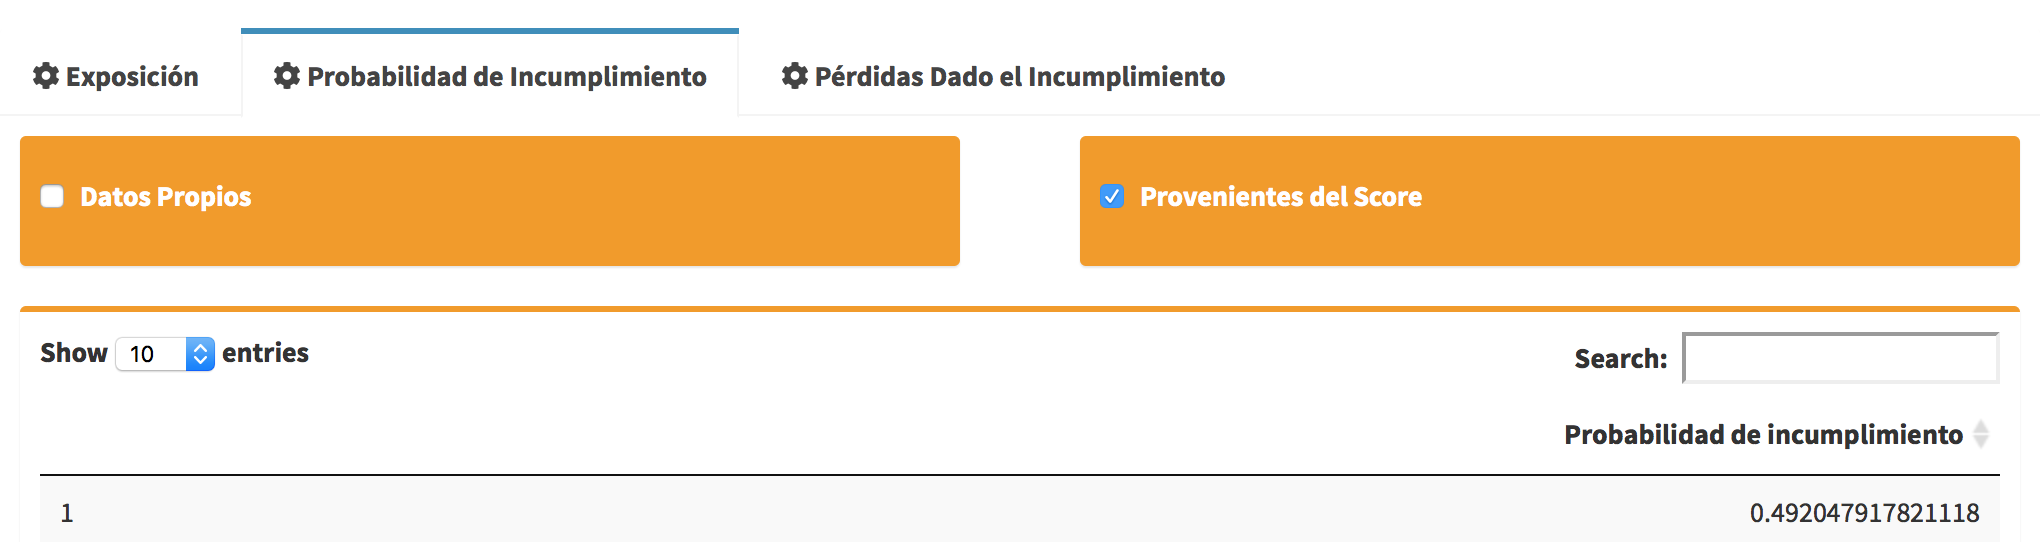
\includegraphics{images/13.png}
\caption{\label{fig:"sd"}}
\end{figure}

\hypertarget{perdidas-dado-el-incumplimiento}{%
\subsubsection{Pérdidas dado el incumplimiento}\label{perdidas-dado-el-incumplimiento}}

Se cargan las pérdidas asociadas a cada cliente o seleccionamos la opción \emph{Pérdidas por Clientes} para asociar una única pérdida a todos por igual.

\begin{figure}
\centering
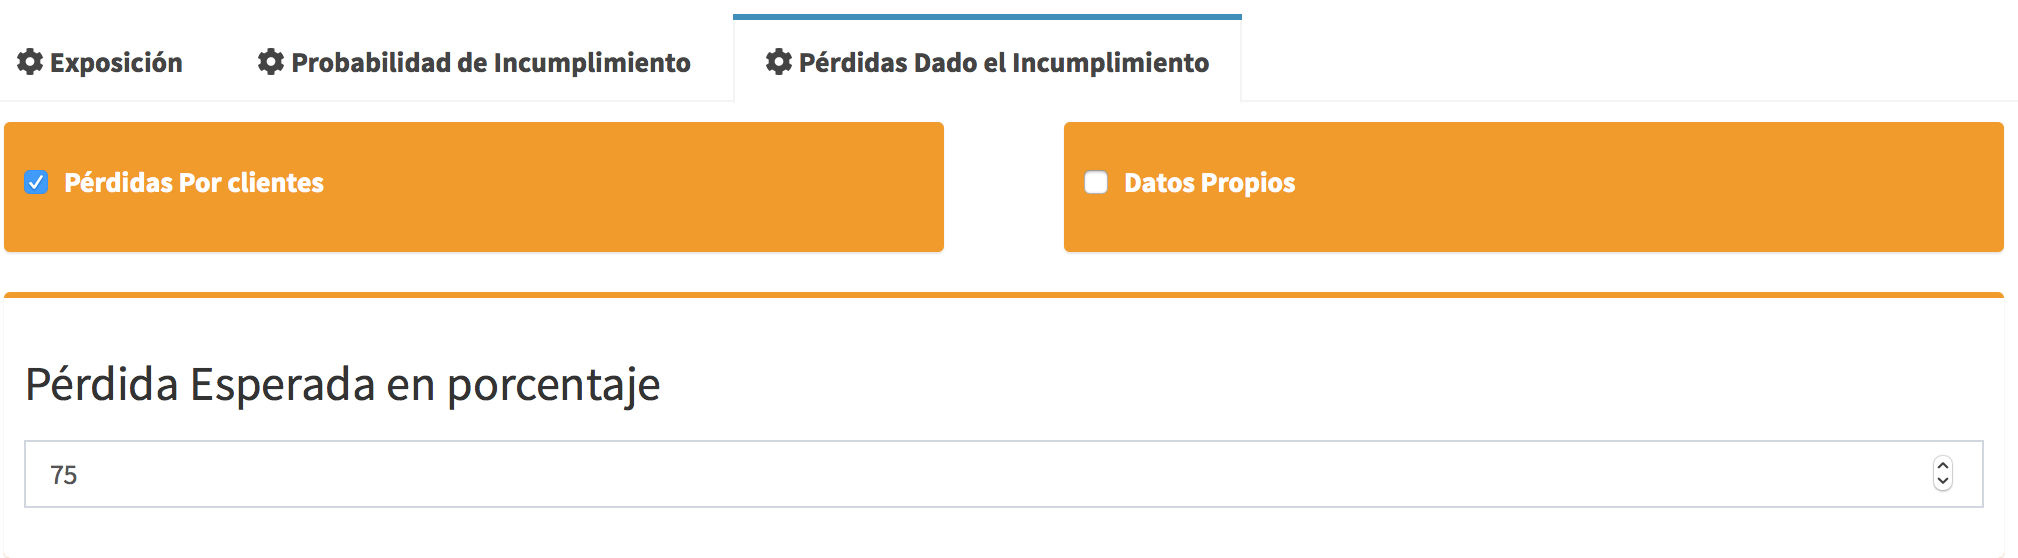
\includegraphics{images/12.png}
\caption{\label{fig:"sd"}}
\end{figure}

\hypertarget{creditmetric}{%
\subsection{CreditMetric}\label{creditmetric}}

En esta sección se cargaran los datos correspondientes a la segunda metodología de riesgo de crédito.

\hypertarget{exposicion-1}{%
\subsubsection{Exposición}\label{exposicion-1}}

Cargamos los datos de las exposiciones de cada cliente y sus calificaciones crediticias.

\begin{figure}
\centering
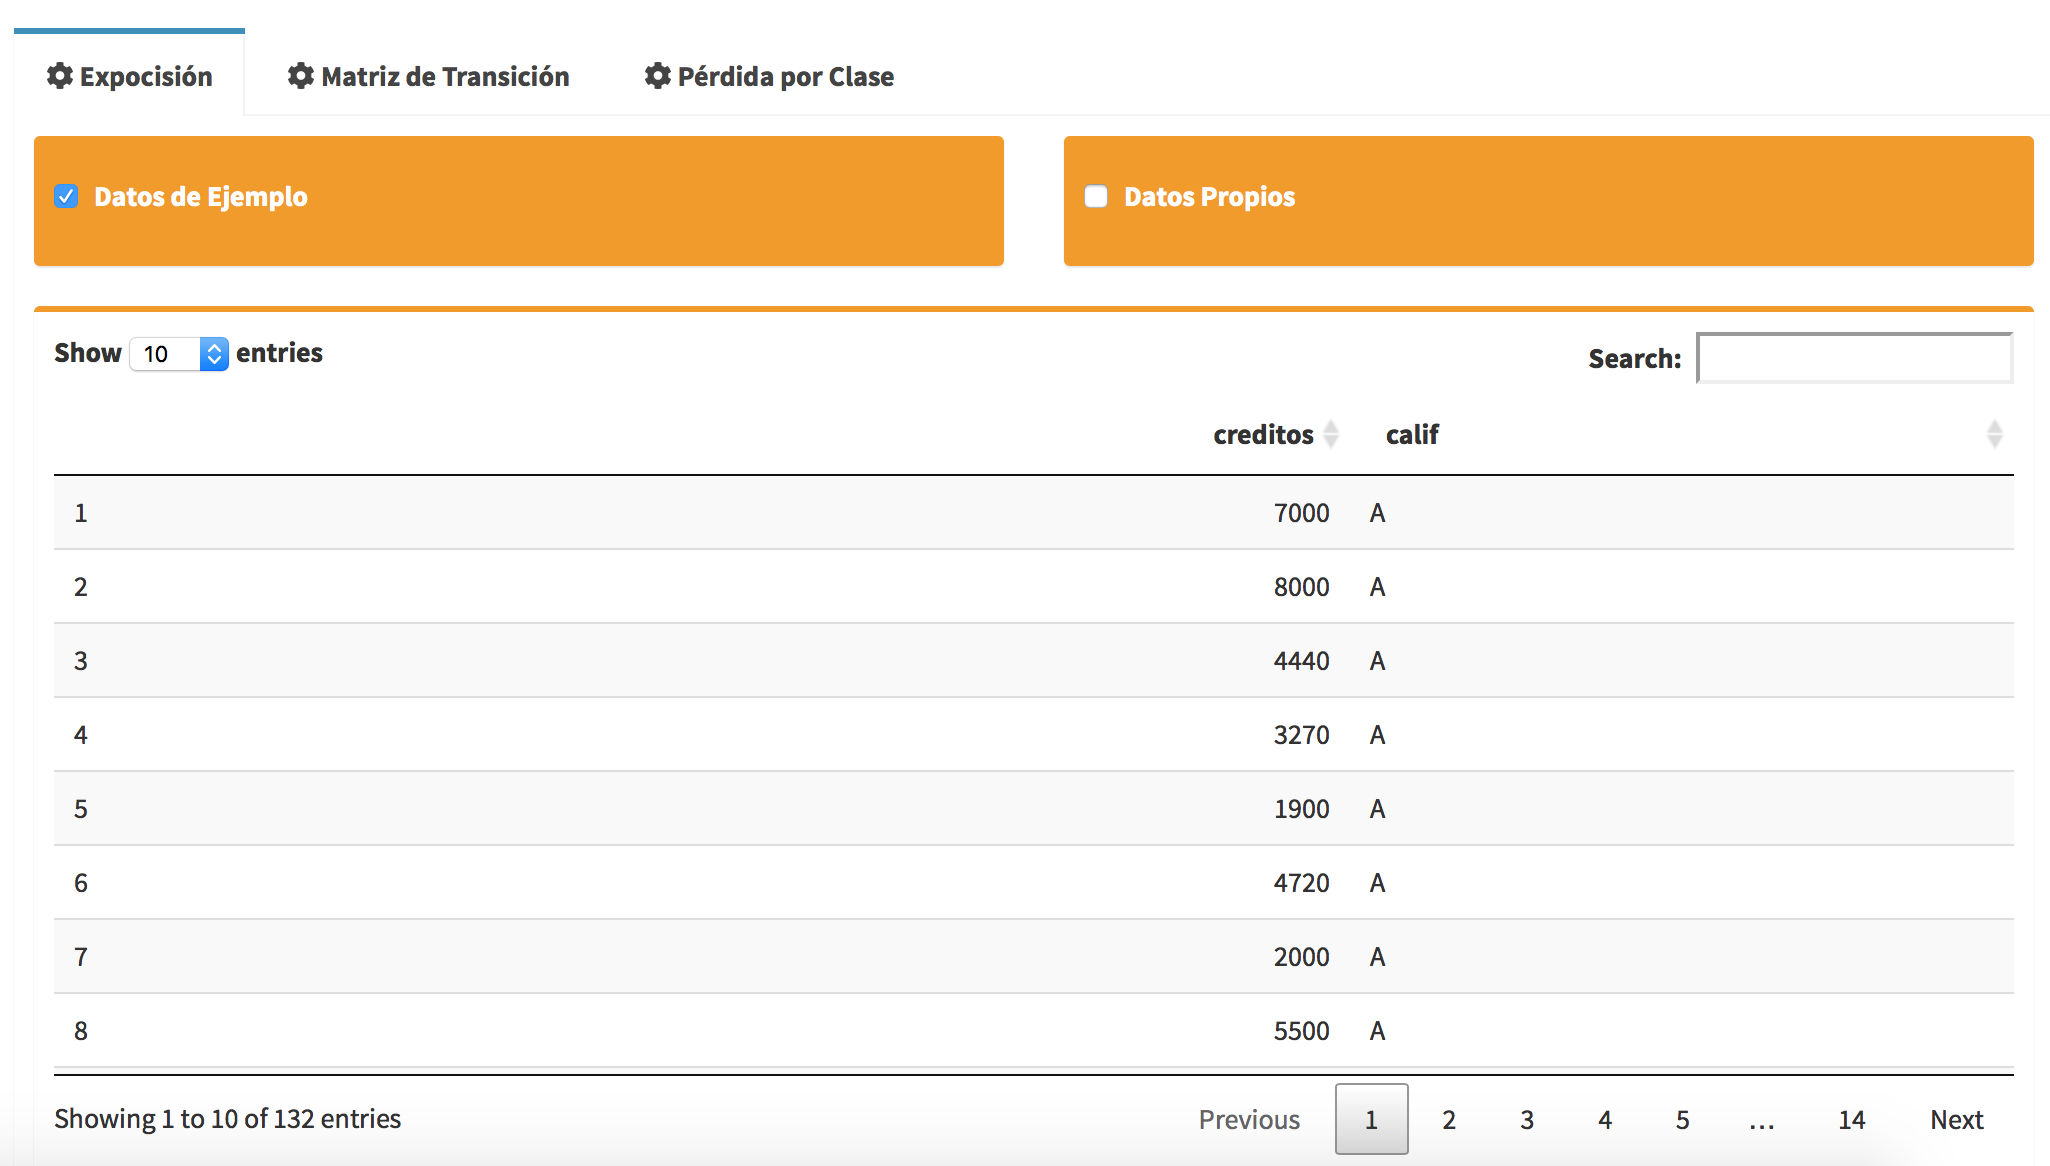
\includegraphics{images/15.png}
\caption{\label{fig:"sd"}}
\end{figure}

\hypertarget{matriz-de-transicion-2}{%
\subsubsection{Matriz de transición}\label{matriz-de-transicion-2}}

Cargamos la matriz de transición, tendremos la opción de cargar la calculada en la sección \emph{Matriz de transición}

\begin{figure}
\centering
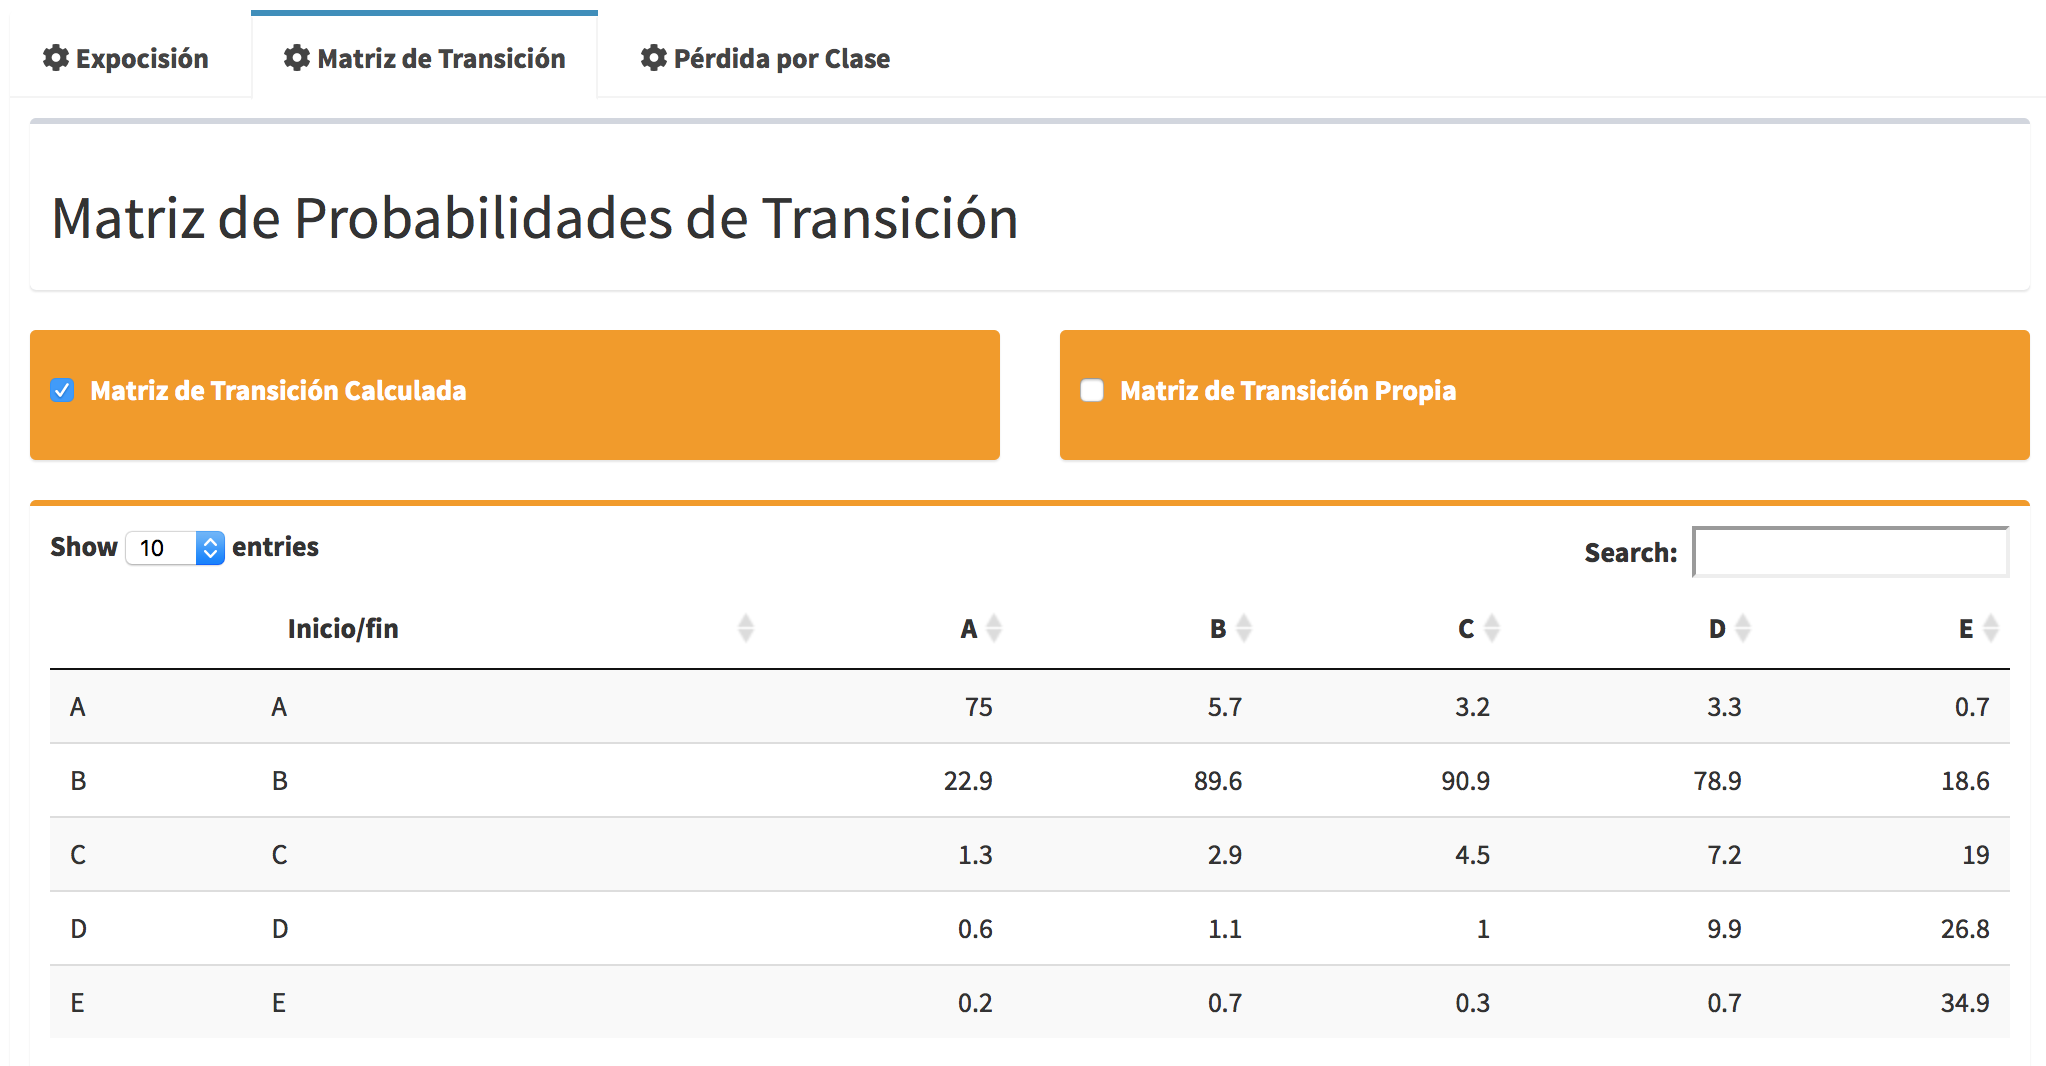
\includegraphics{images/16.png}
\caption{\label{fig:"sd"}}
\end{figure}

\hypertarget{perdidas-dado-el-incumplimiento-1}{%
\subsubsection{Pérdidas dado el incumplimiento}\label{perdidas-dado-el-incumplimiento-1}}

Cargamos las pérdidas esperadas por categoría, de igual forma tenemos la opción de usar la calculada en la sección \emph{Pérdida por incumplimiento}

\begin{figure}
\centering
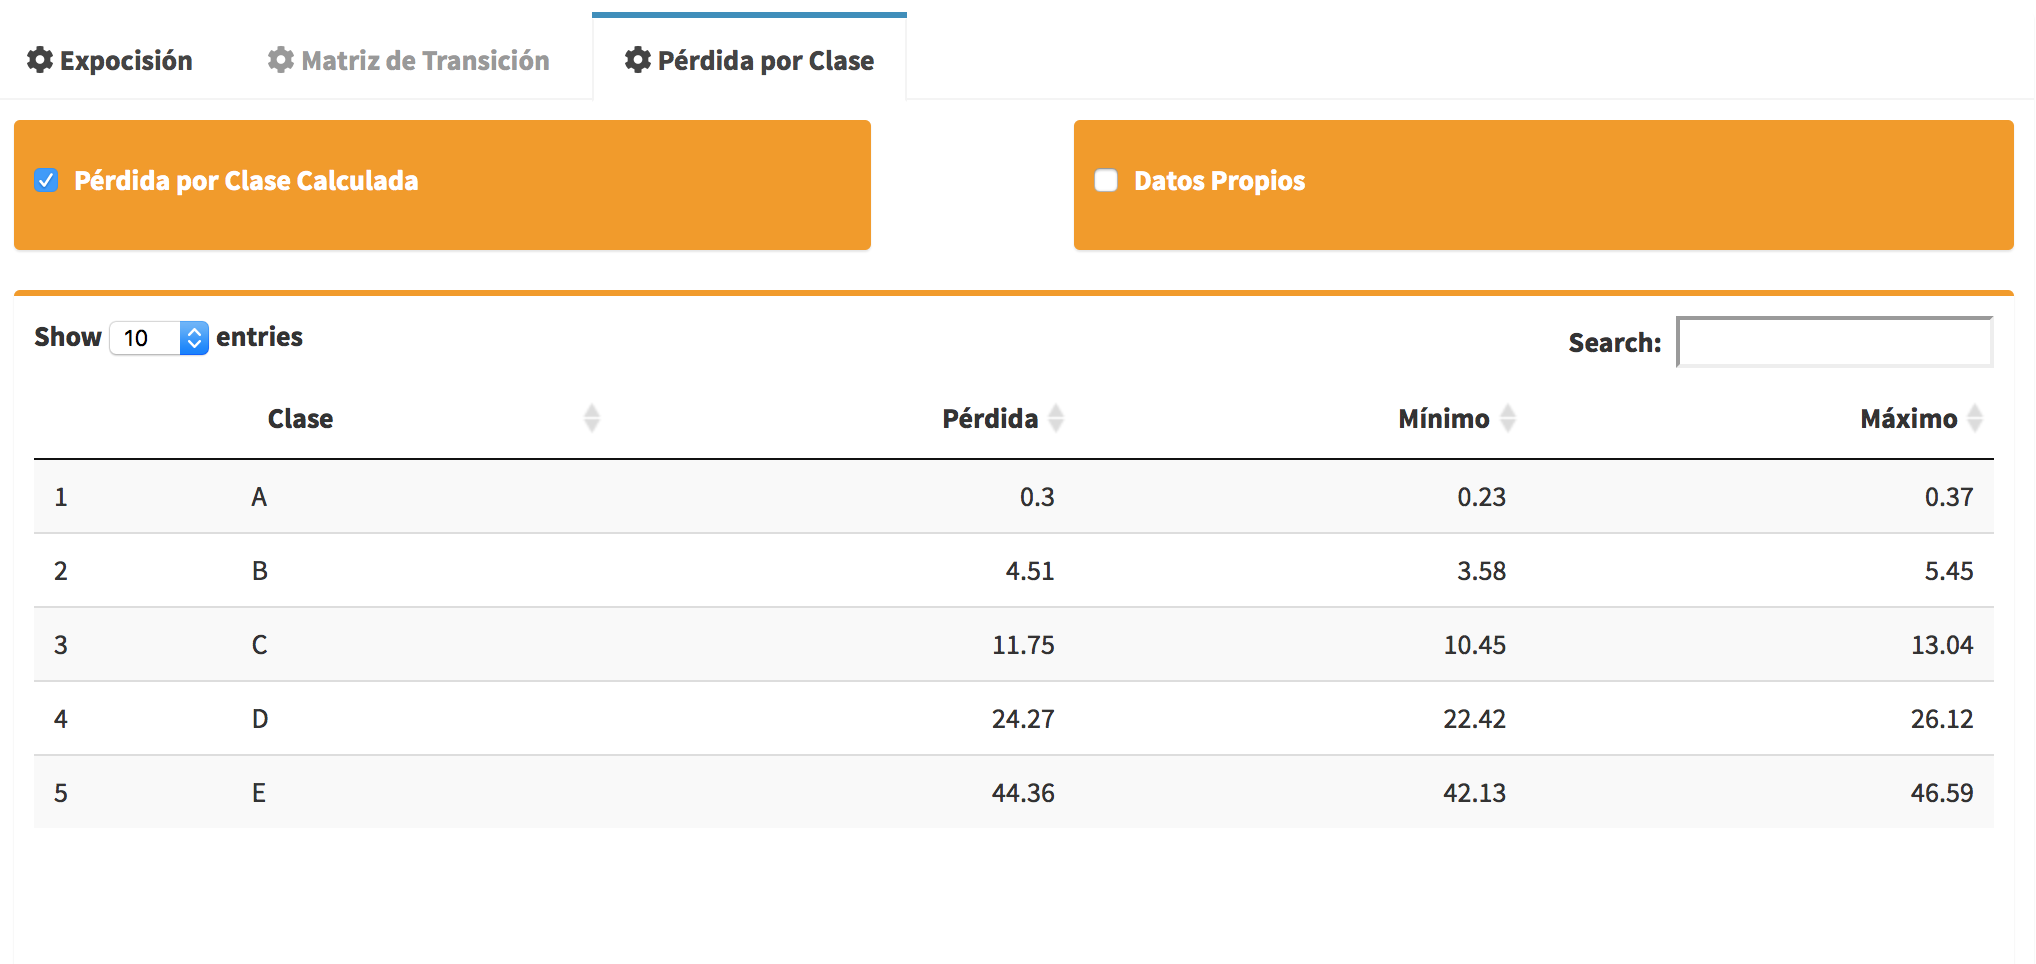
\includegraphics{images/17.png}
\caption{\label{fig:"sd"}}
\end{figure}

\hypertarget{backtesting}{%
\subsection{BackTesting}\label{backtesting}}

En esta sección cargamos los datos para realizar puebas al VaR

\begin{figure}
\centering
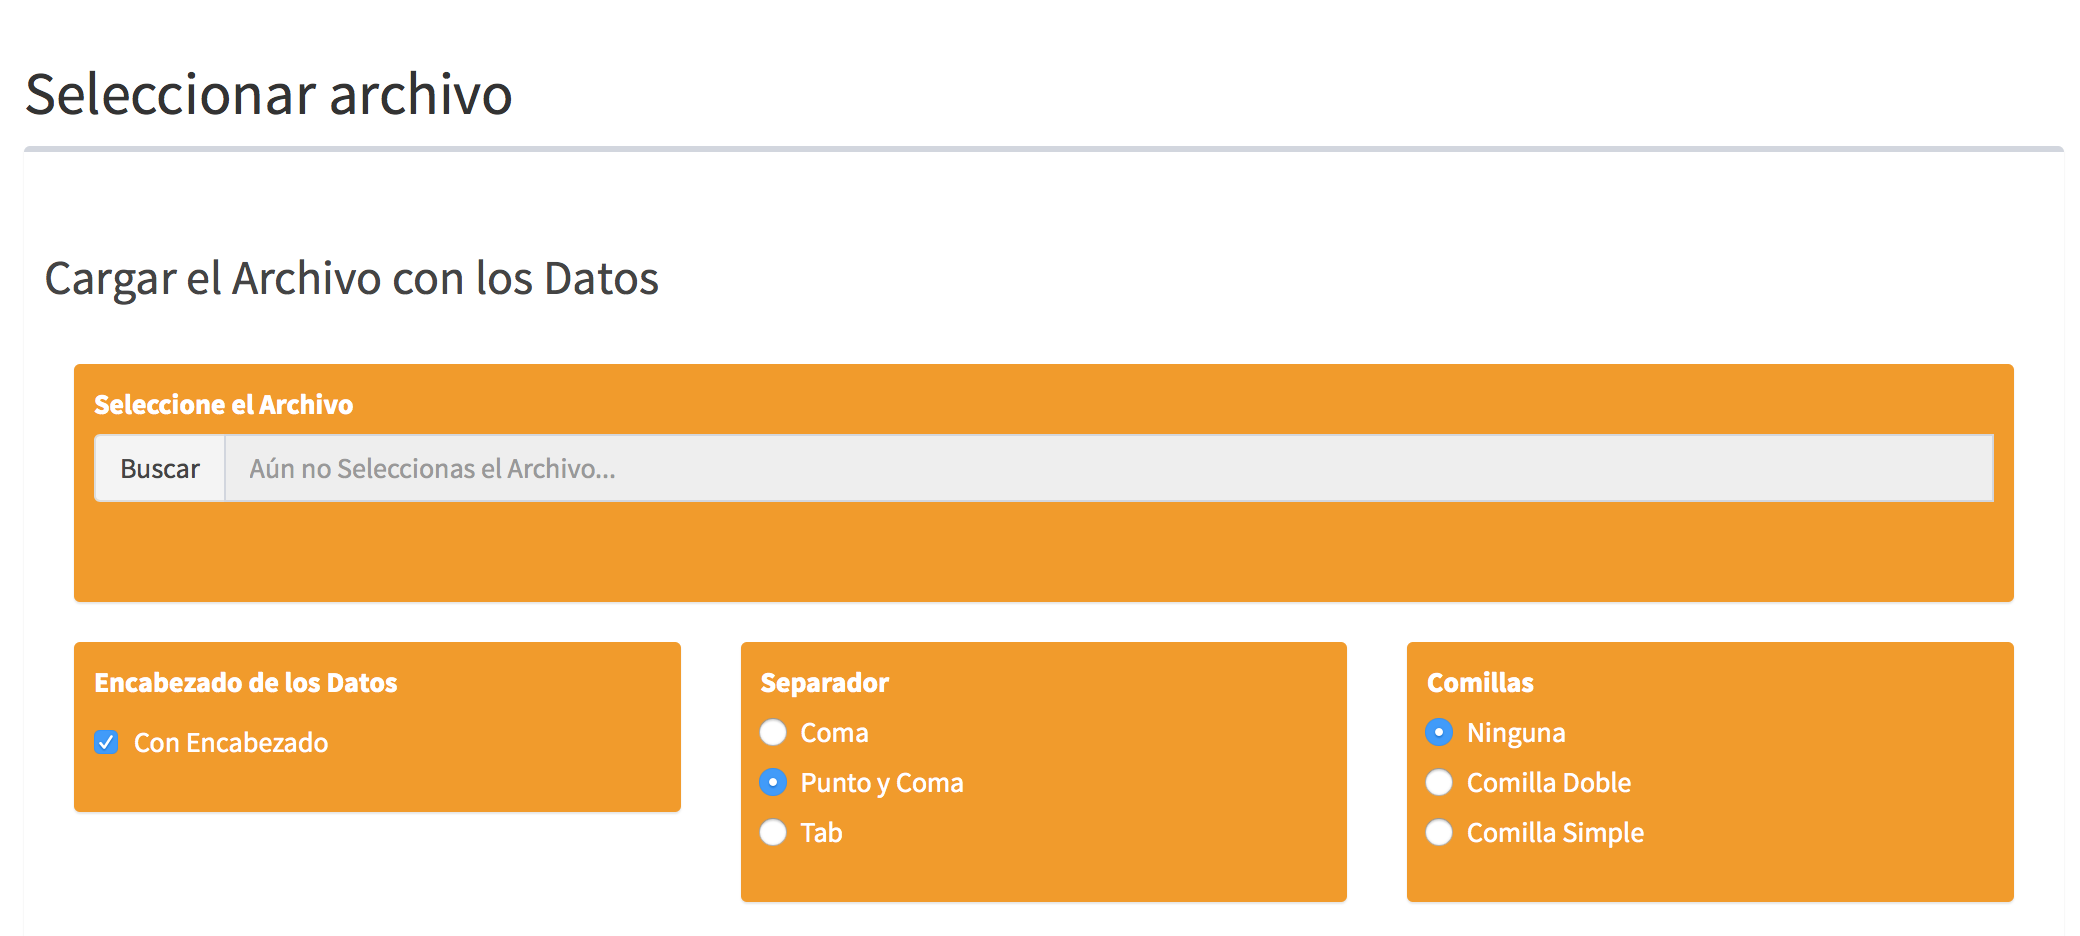
\includegraphics{images/19.png}
\caption{\label{fig:"sd"}}
\end{figure}

\hypertarget{indicadores-contables}{%
\subsection{Indicadores Contables}\label{indicadores-contables}}

En esta sección se calcularán algunos indicadores contables, primero debemos seleccionar que metodología se usará y luego cargar el archivo con ciertos datos contables.

\begin{figure}
\centering
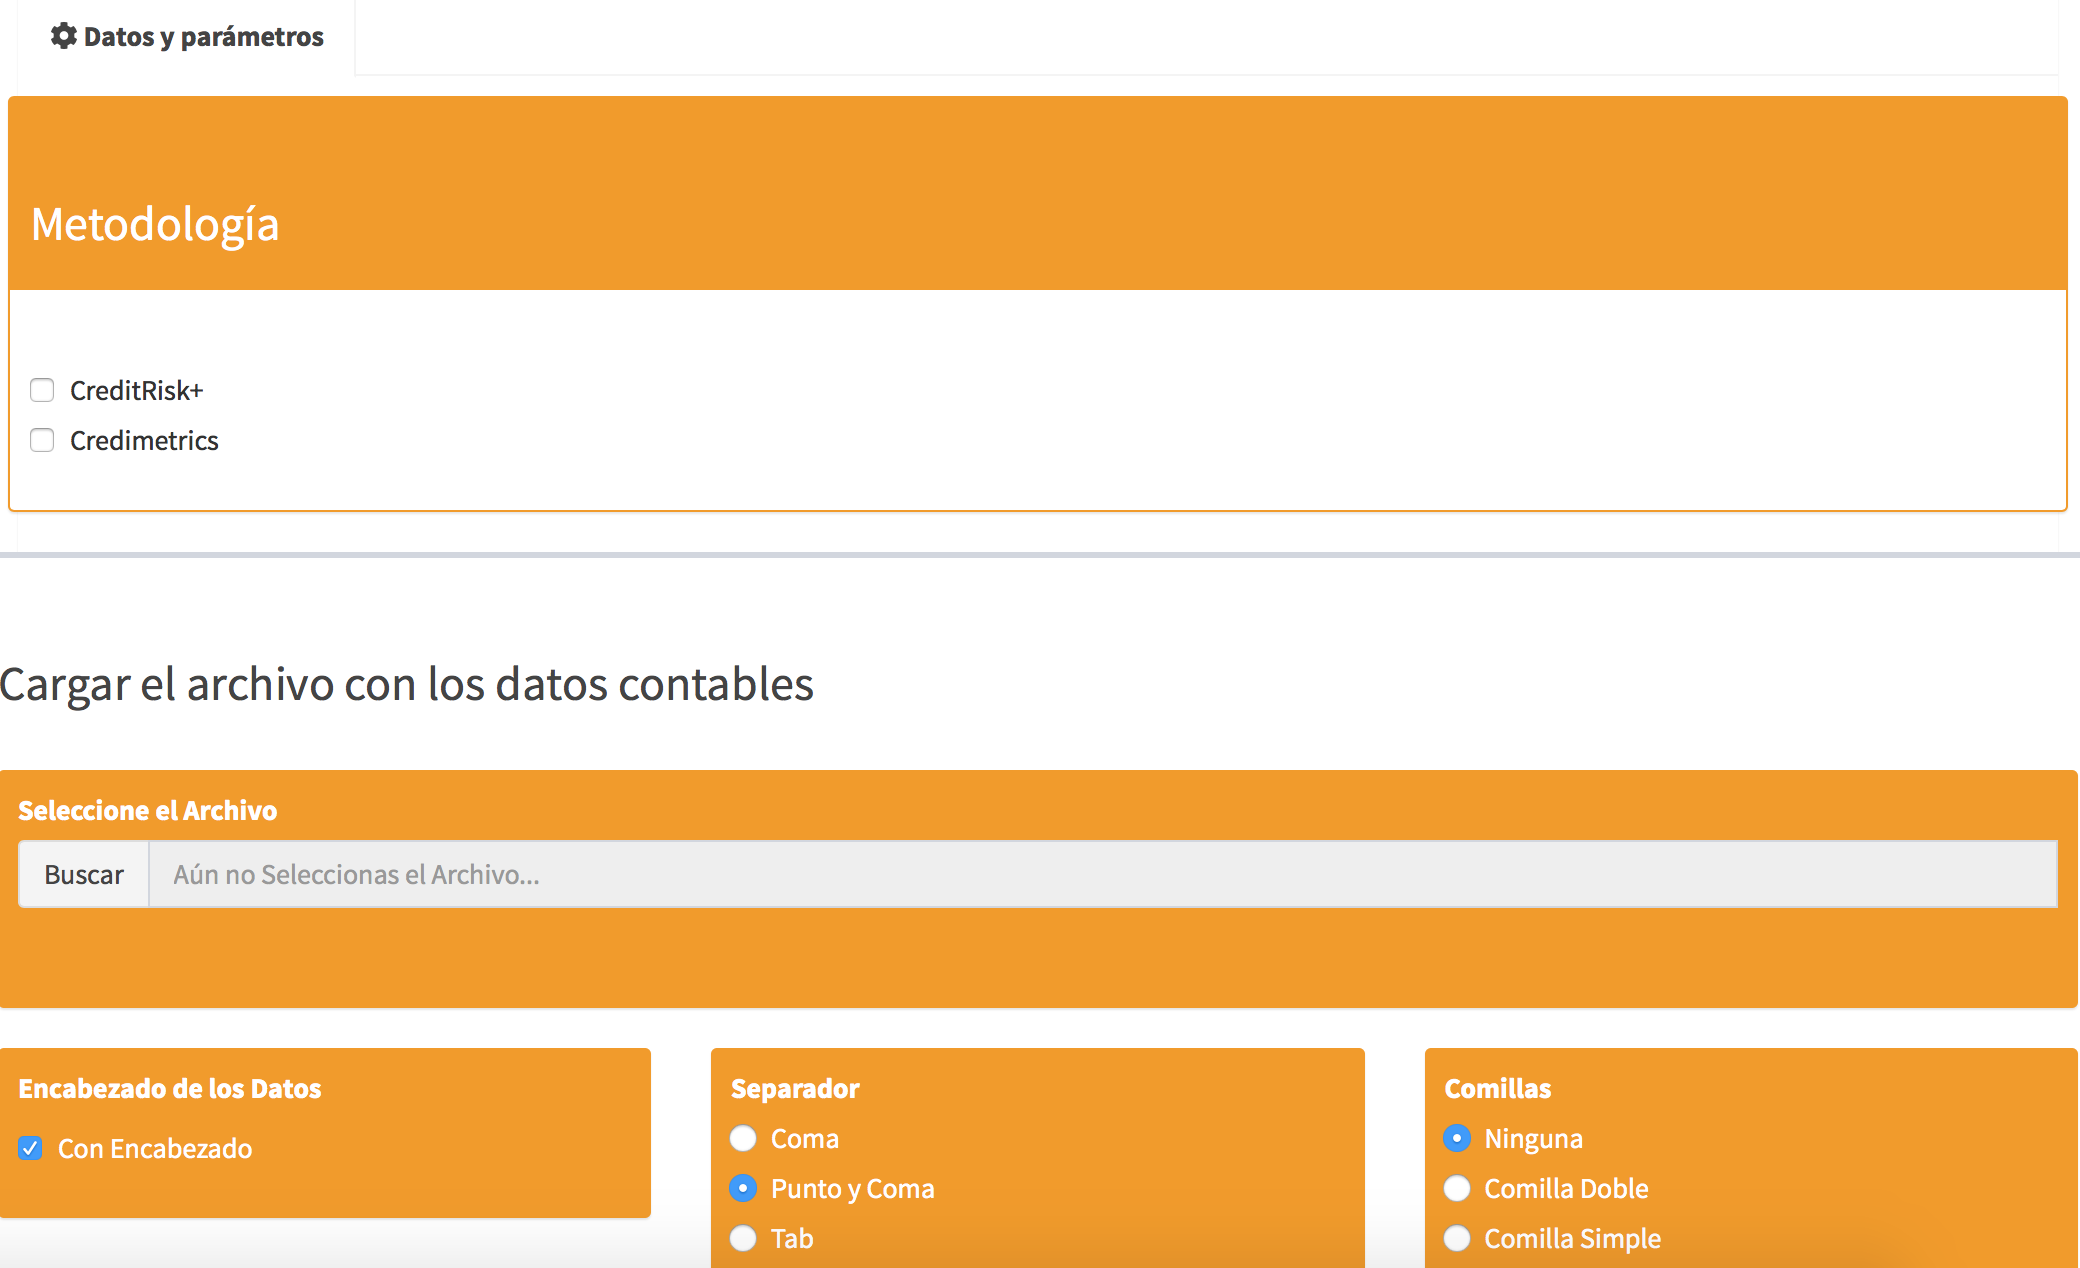
\includegraphics{images/18.png}
\caption{\label{fig:"sd"}}
\end{figure}

\hypertarget{score-y-rating}{%
\section{Score y rating}\label{score-y-rating}}

Esta sección esta conformada por tres pestañas, estadísticos, Score de crédito y Rating de crédito

\begin{figure}
\centering
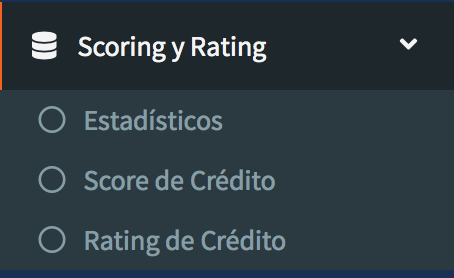
\includegraphics{images/20.png}
\caption{\label{fig:"sd"}}
\end{figure}

\hypertarget{estadisticos}{%
\subsection{Estadísticos}\label{estadisticos}}

Em esta sección veremos un pequeño resumen estadísticos y criterios para la selección de variables

\hypertarget{relacion-de-las-variables-independientes}{%
\subsubsection{Relación de las variables independientes}\label{relacion-de-las-variables-independientes}}

Se tendrá la opción de ver el gráfico de caja y bigote de la variable independiente seleccionada y la variable Default. Además se tendrá un resumen estadístico de la variable seleccionada.

\begin{figure}
\centering
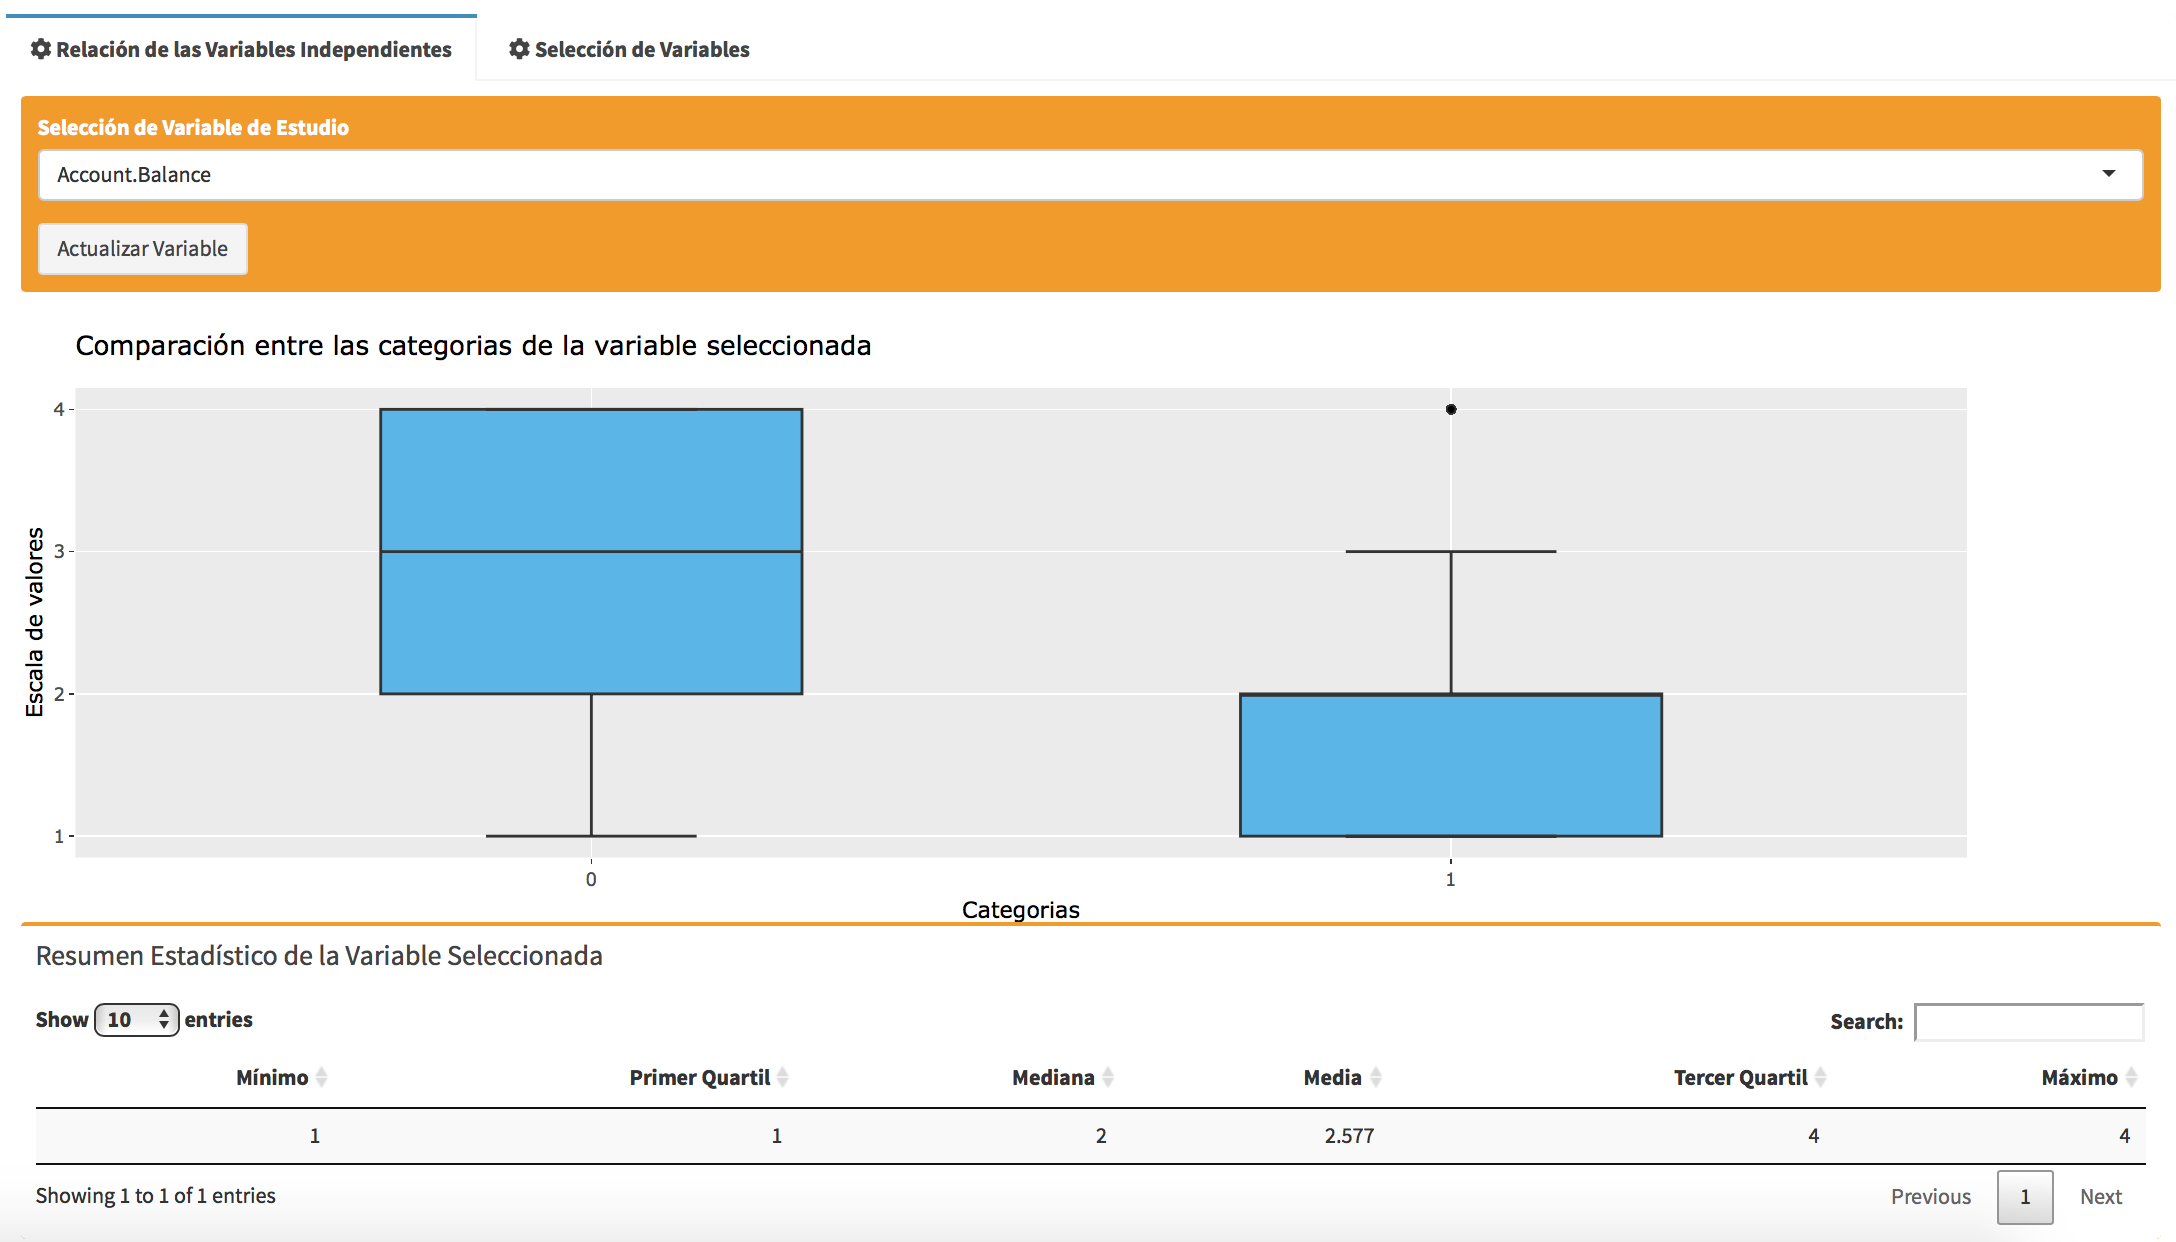
\includegraphics{images/21.png}
\caption{\label{fig:"sd"}}
\end{figure}

\hypertarget{seleccion-de-variables}{%
\subsubsection{Selección de variables}\label{seleccion-de-variables}}

Tendremos dos opciones, las cuales corresponden a la selección de variables cualitativas y cuantitativas, una vez seleccionada la opción podremos escoger el nivel de significancia de la prueba.

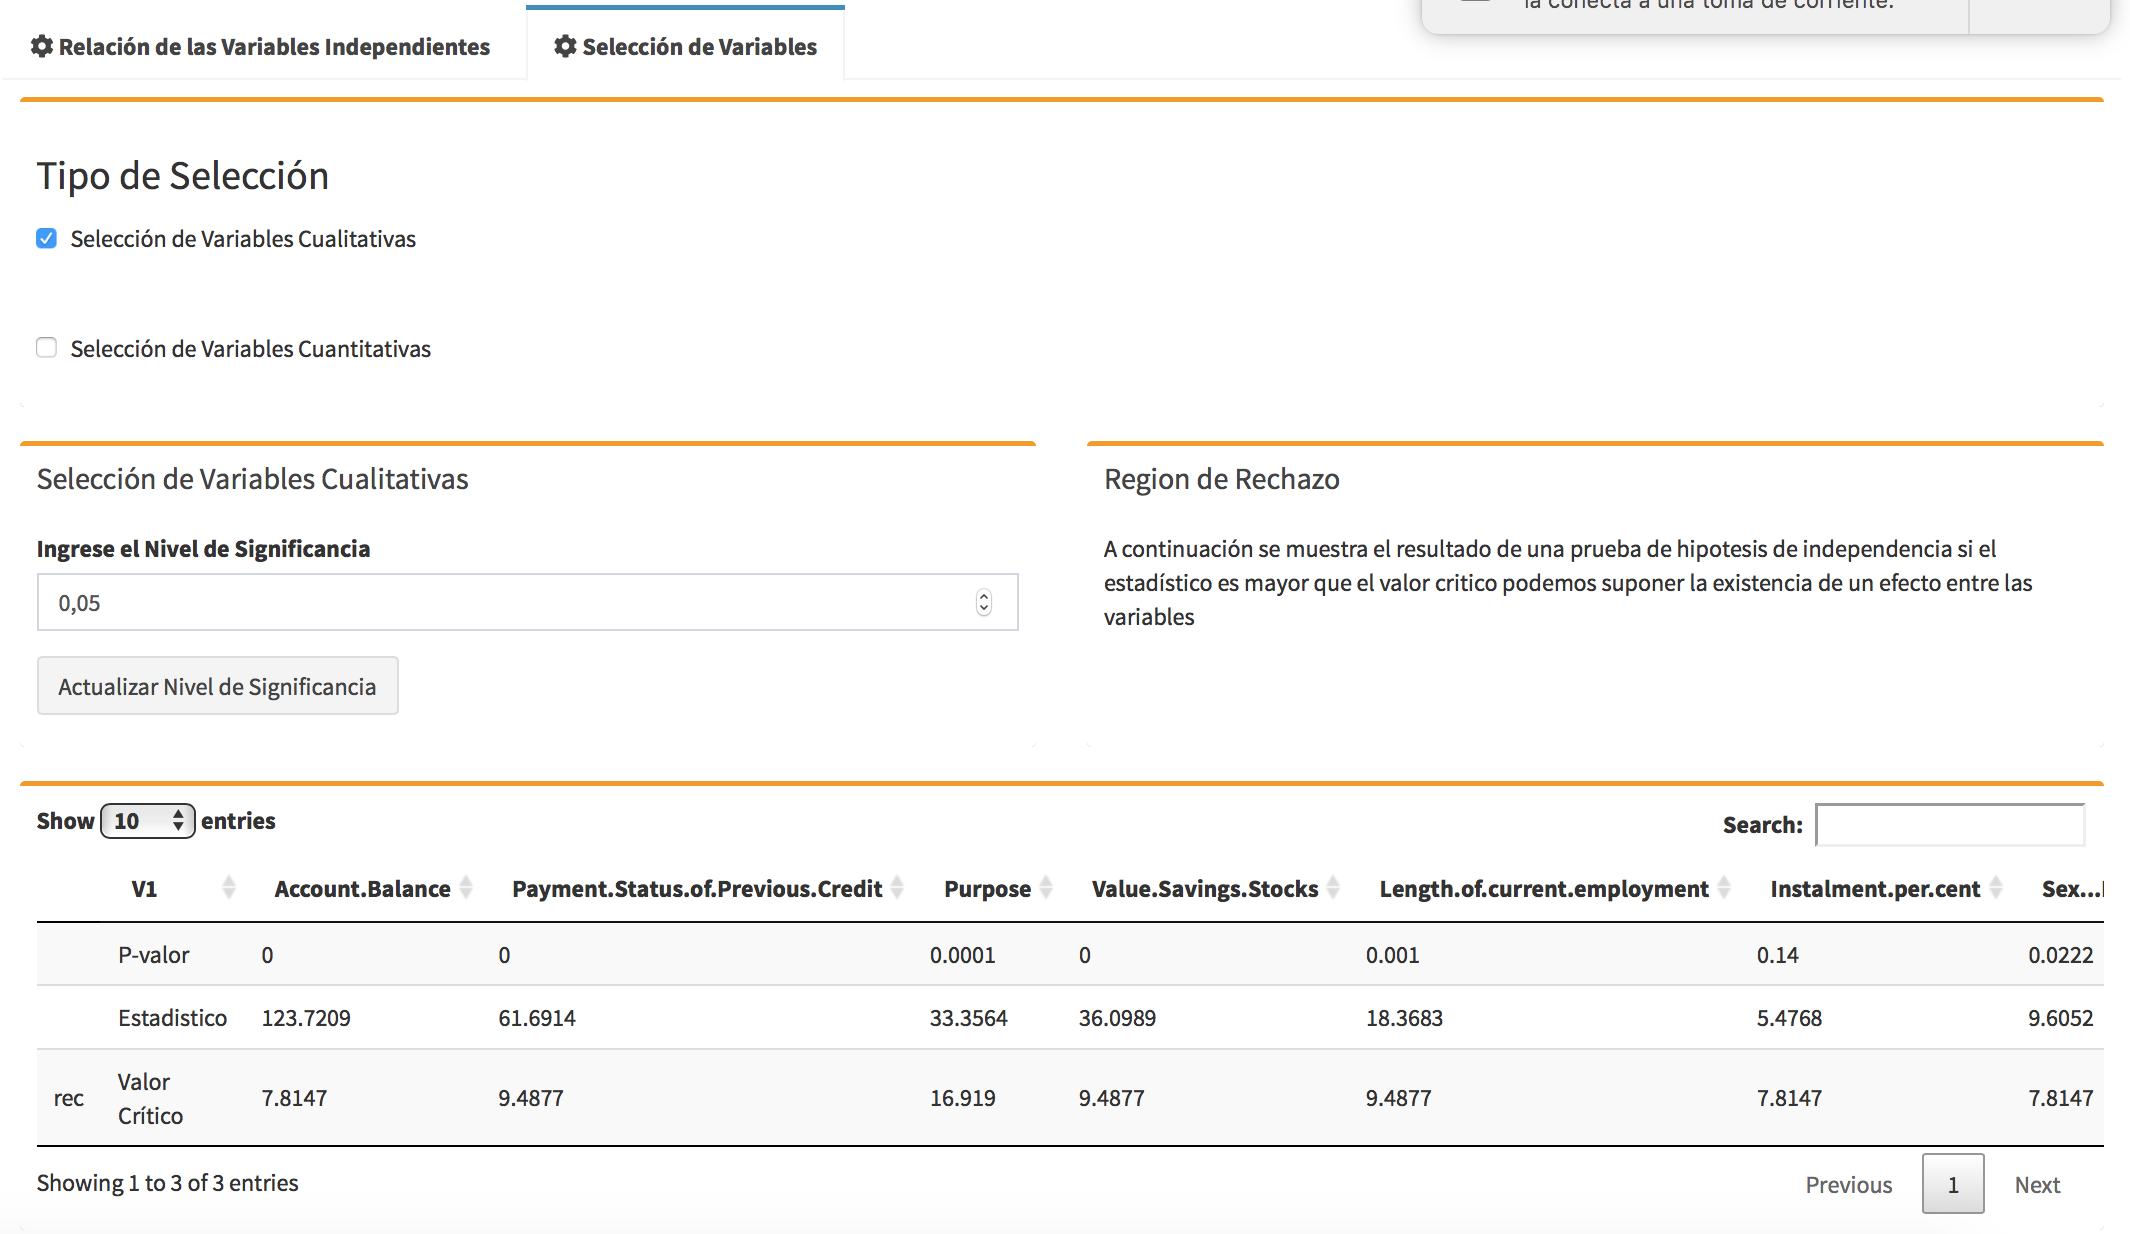
\includegraphics{images/22.png}
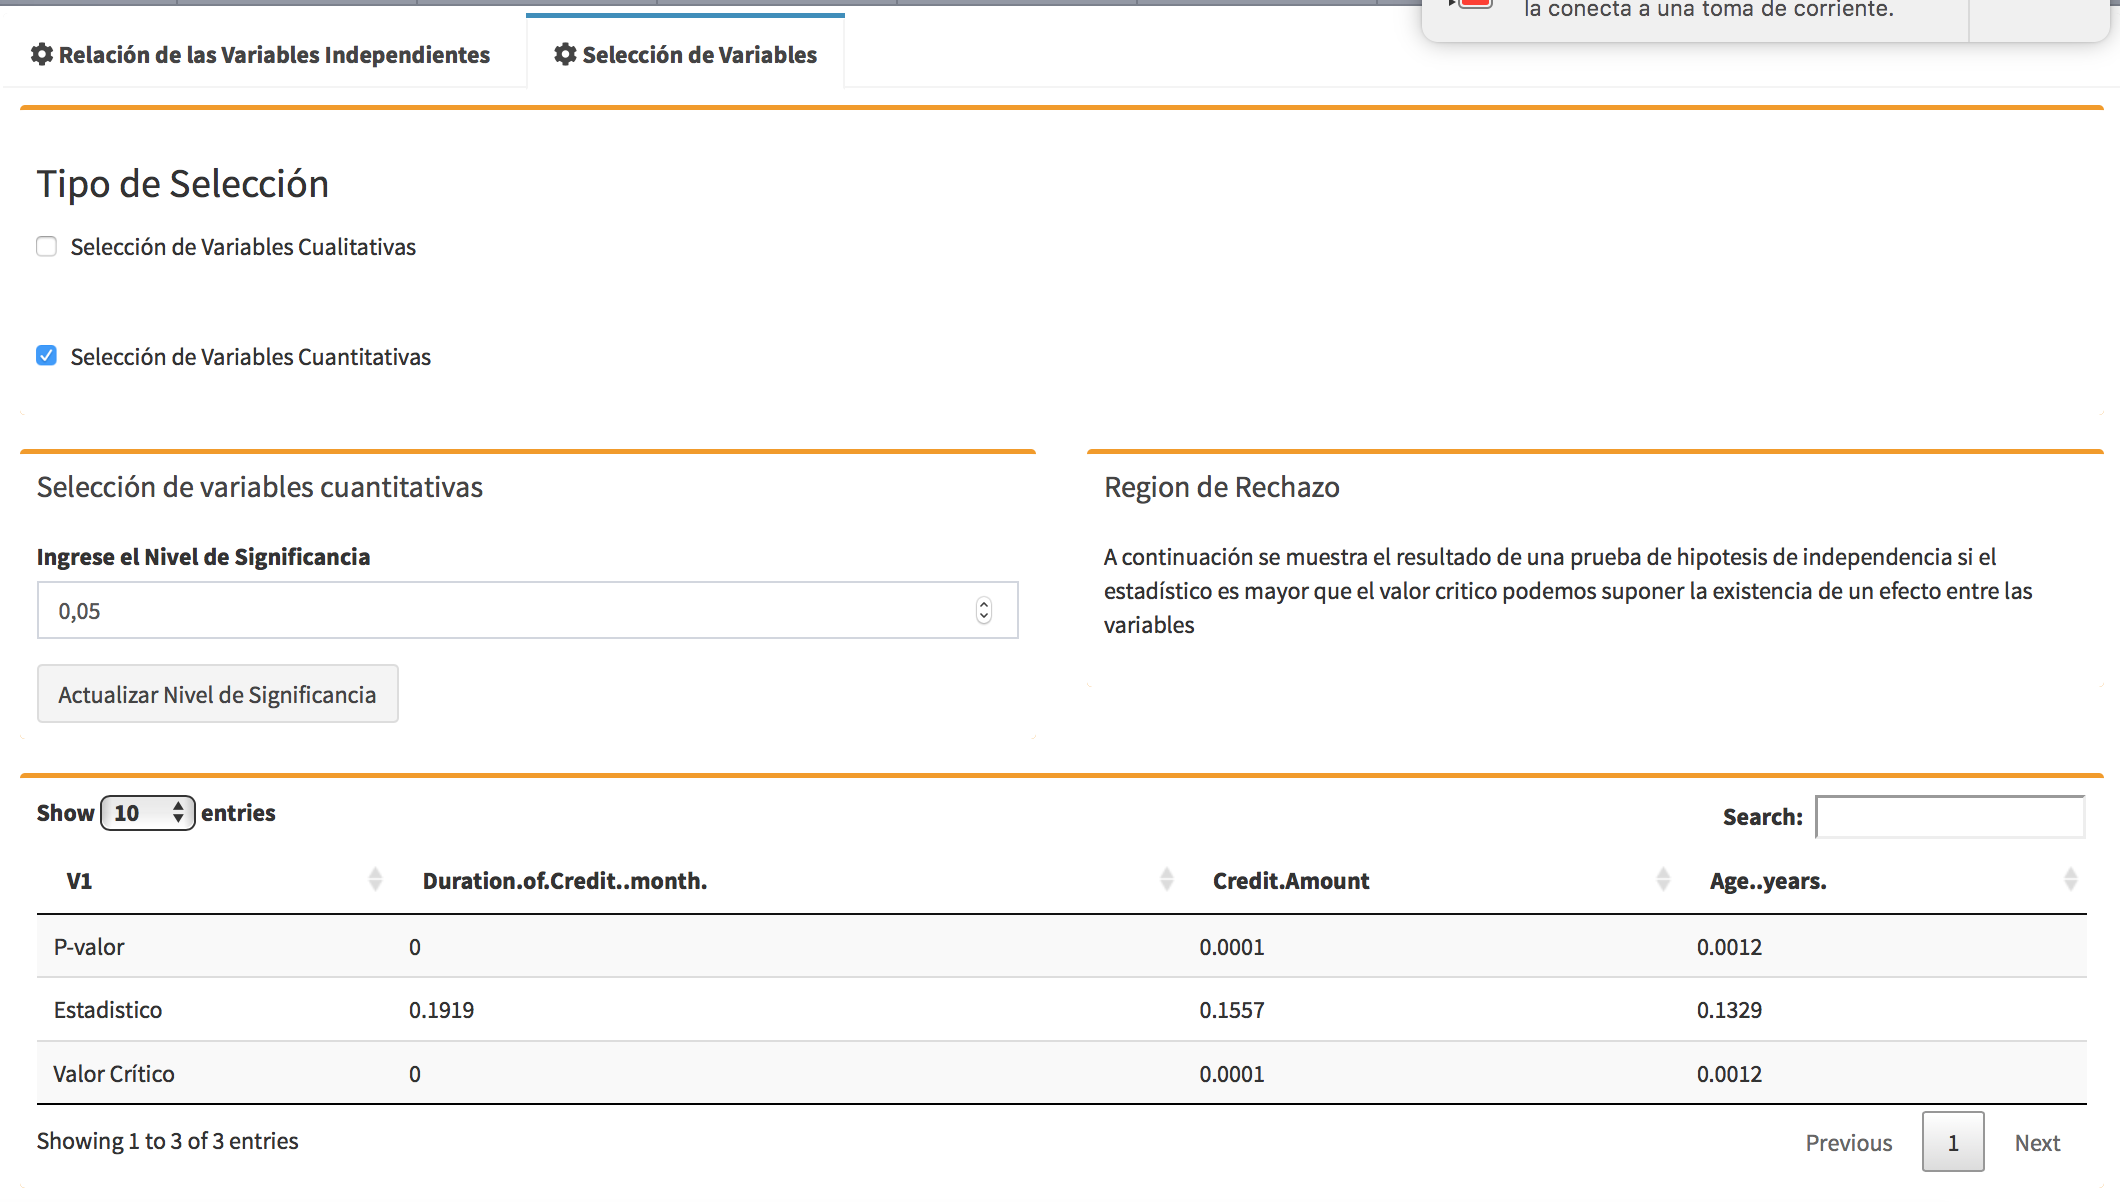
\includegraphics{images/23.png}

\hypertarget{score-de-credito}{%
\subsection{Score de Crédito}\label{score-de-credito}}

En esta sección contruiremos el \emph{Score} de crédito el cual está basado en un modelo lineal generalizado.

\hypertarget{seleccion-y-resultado-del-modelo}{%
\subsubsection{Selección y Resultado del modelo}\label{seleccion-y-resultado-del-modelo}}

Primero debemos seleccionar el link del modelo lineal generalizado.

\begin{figure}
\centering
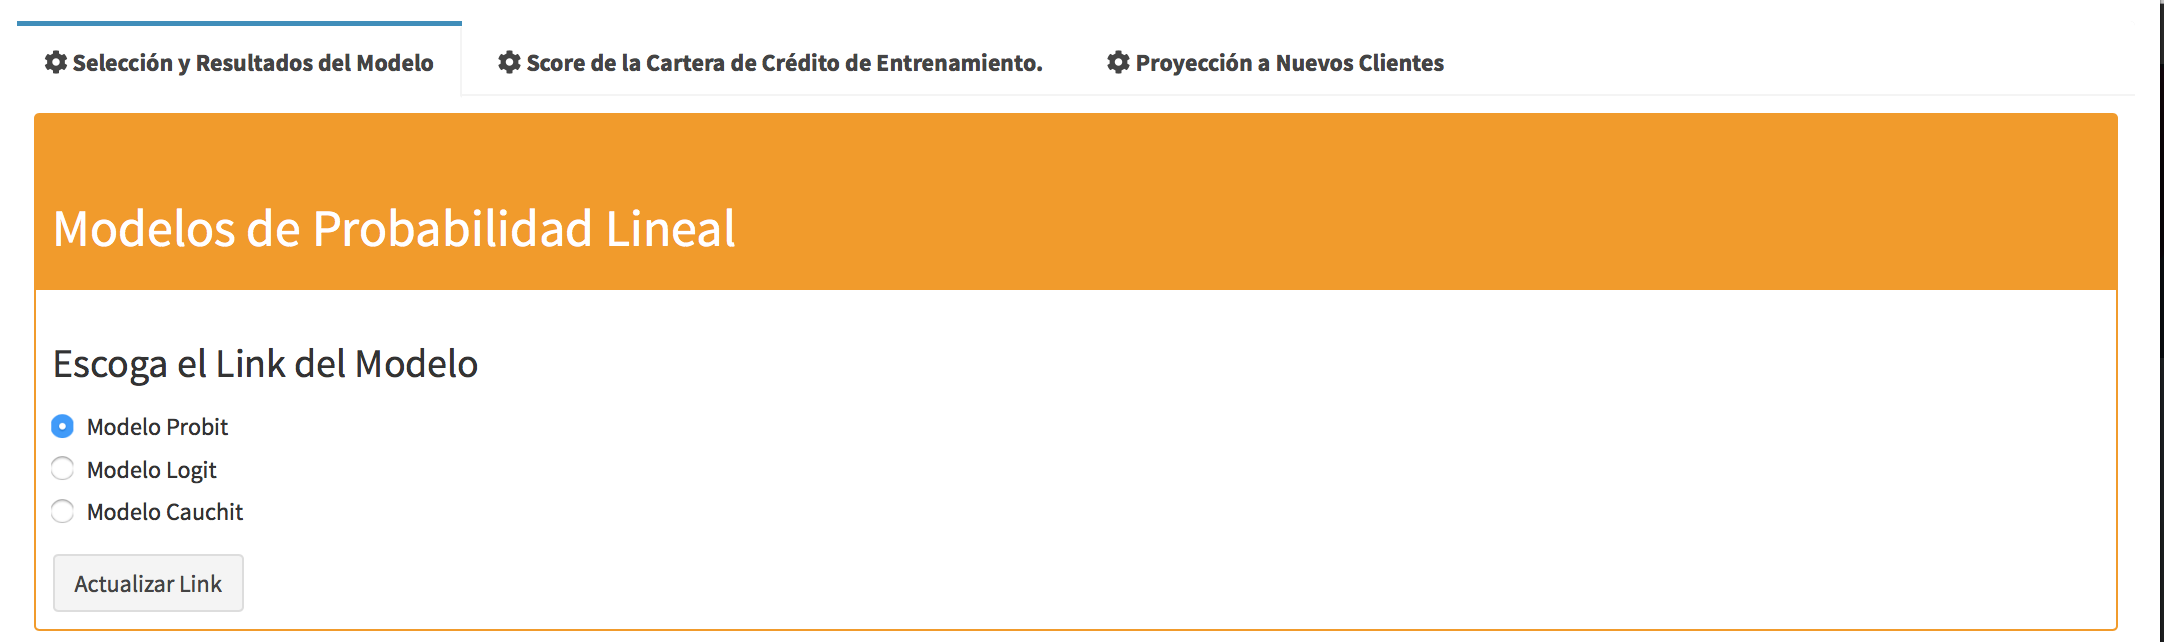
\includegraphics{images/24.png}
\caption{\label{fig:"sd"}}
\end{figure}

Una vez escogido el link se muestrán los coeficientes del modelos por variable.

\begin{figure}
\centering
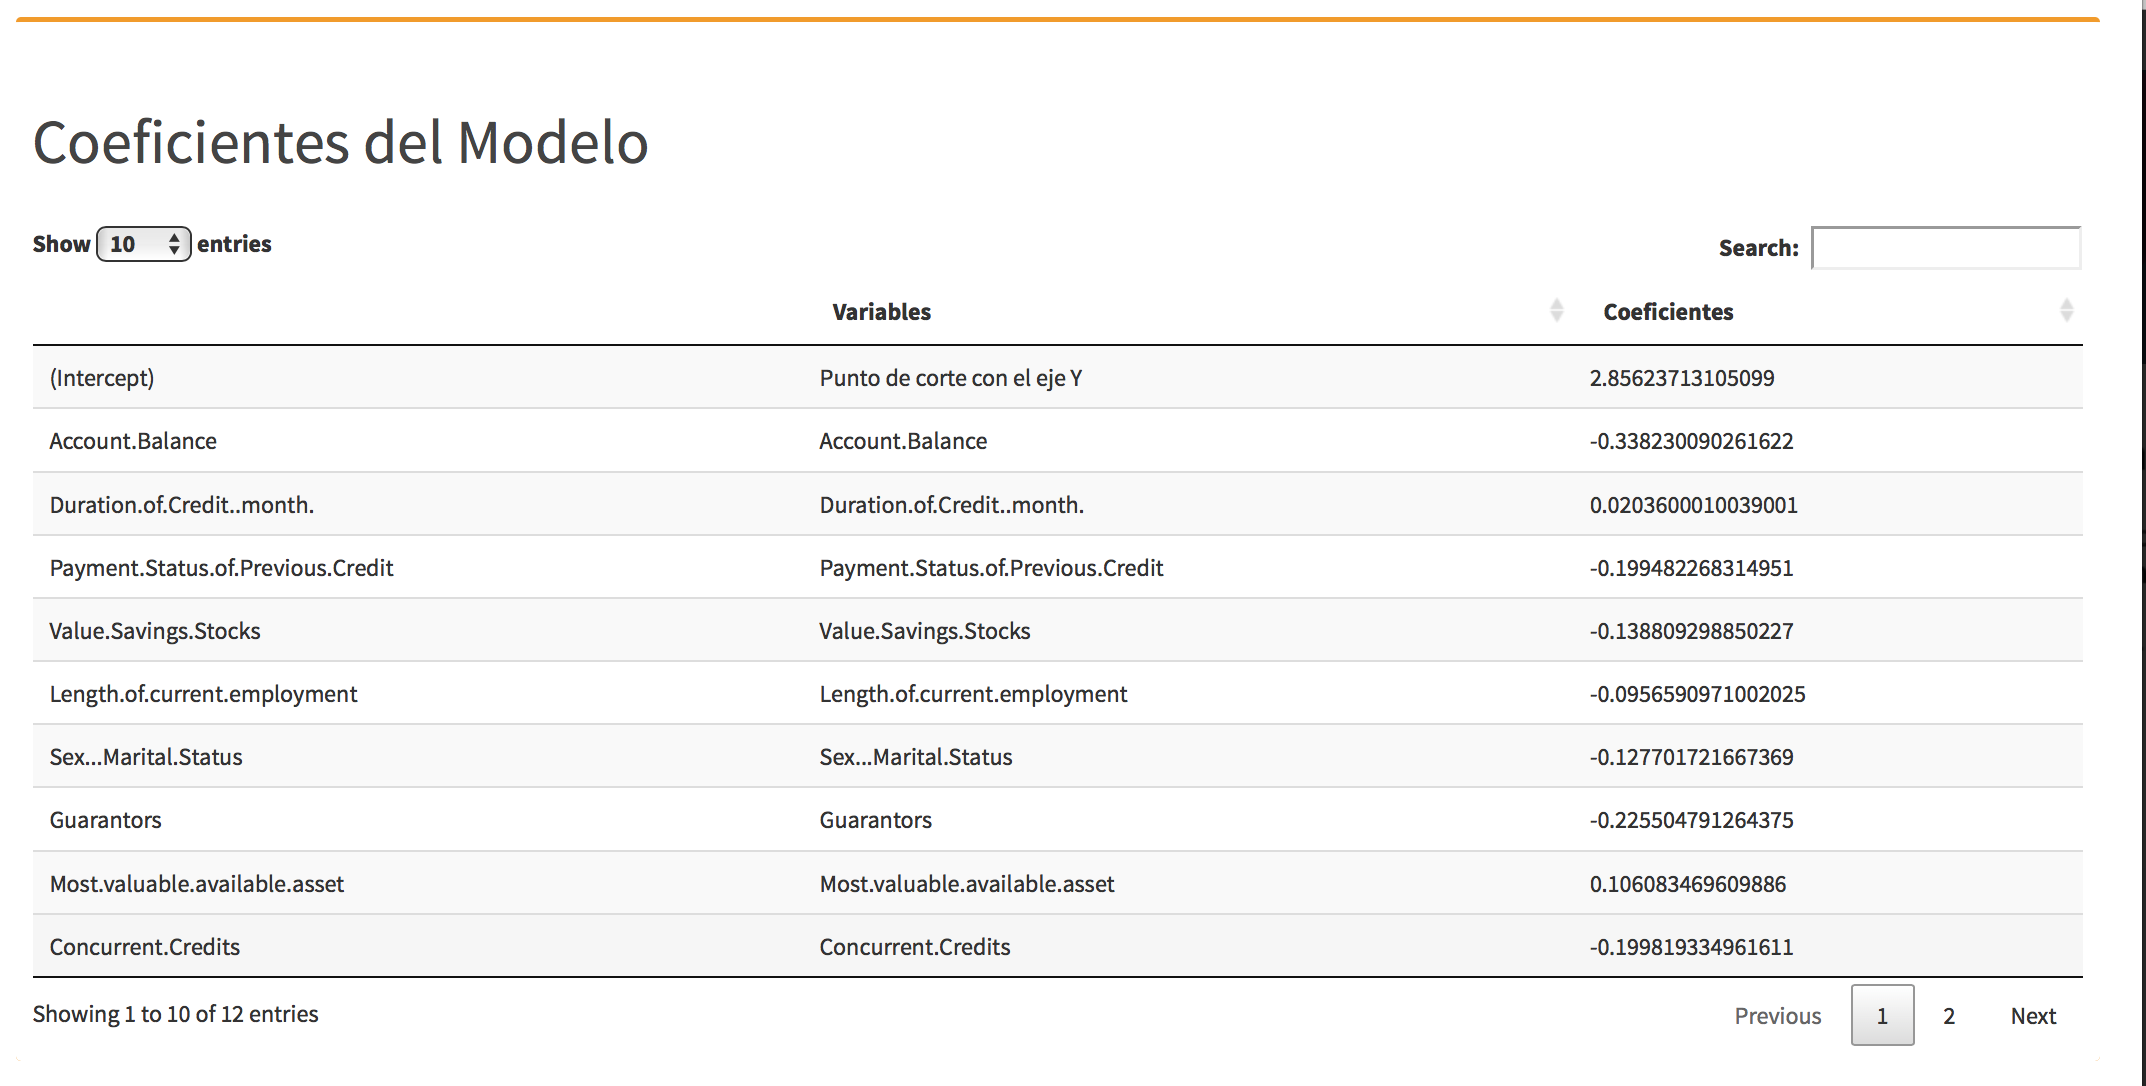
\includegraphics{images/25.png}
\caption{\label{fig:"sd"}}
\end{figure}

Luego se muestra información del modelo en general.

\begin{figure}
\centering
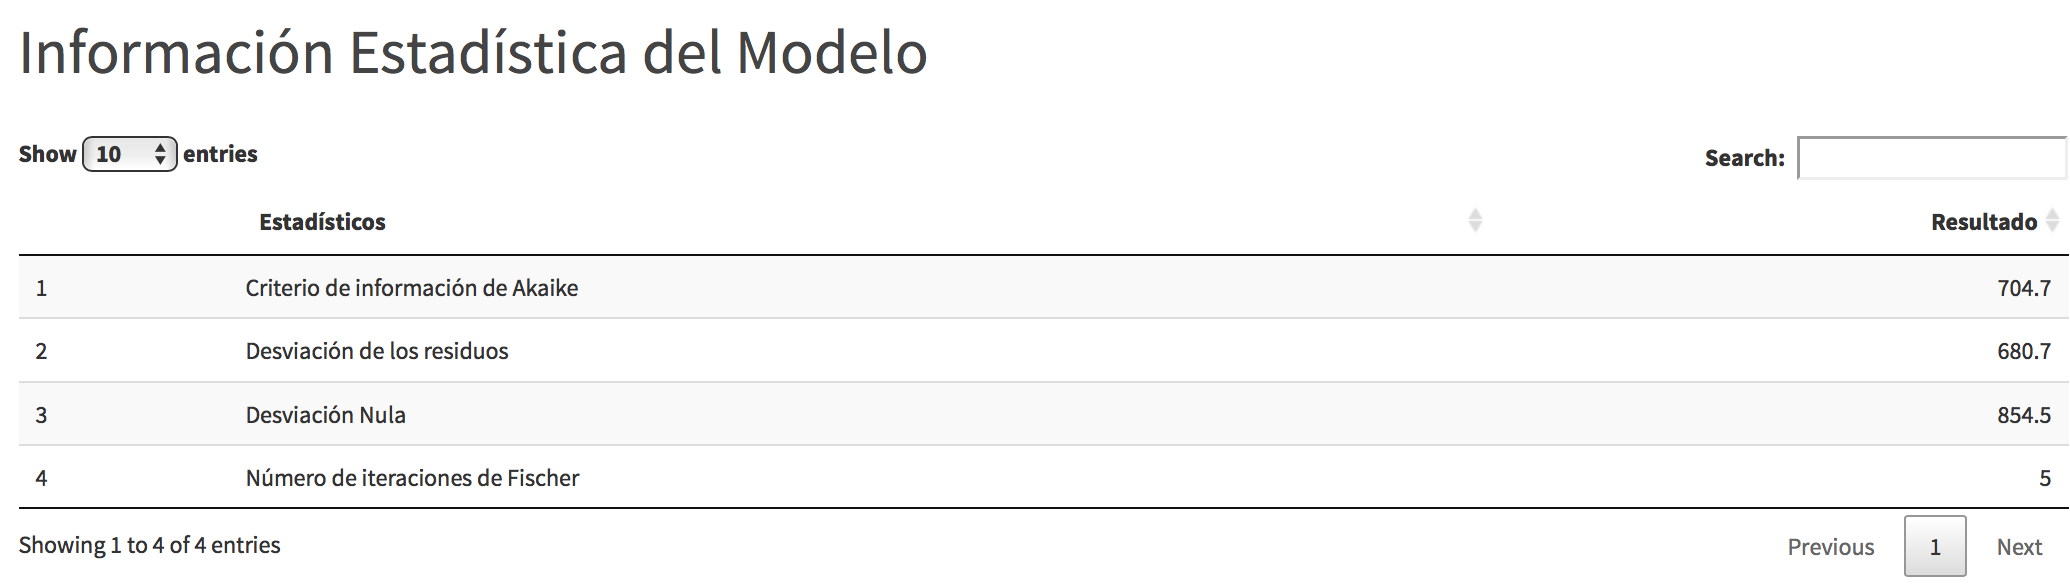
\includegraphics{images/26.png}
\caption{\label{fig:"sd"}}
\end{figure}

Finalizando con información de las métricas de bondad del modelo.
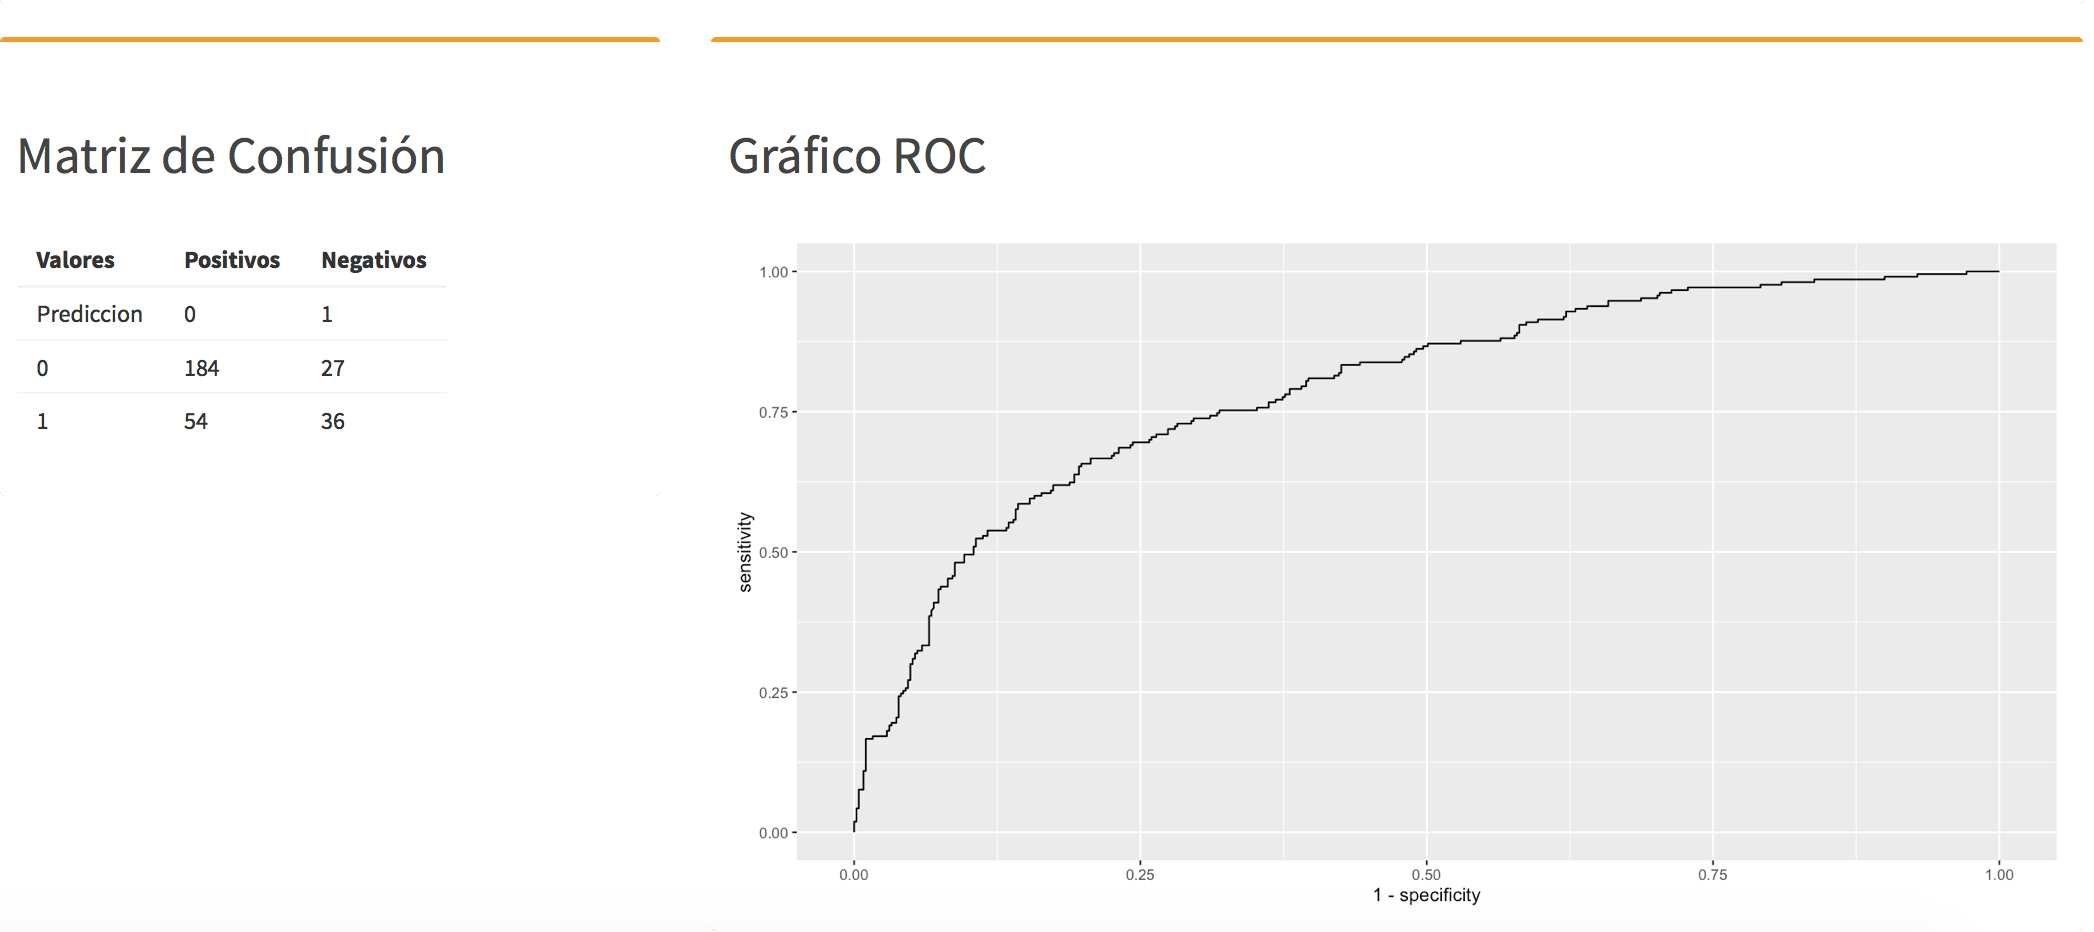
\includegraphics{images/27.png}

\hypertarget{score-de-la-cartera-de-credito-de-entrenamiento}{%
\subsubsection{Score de la cartera de crédito de entrenamiento}\label{score-de-la-cartera-de-credito-de-entrenamiento}}

En esta sección se muestra el Score y probabilidad de incumplimiento de los clientes con los cuales se construyó el modelo.

\begin{figure}
\centering
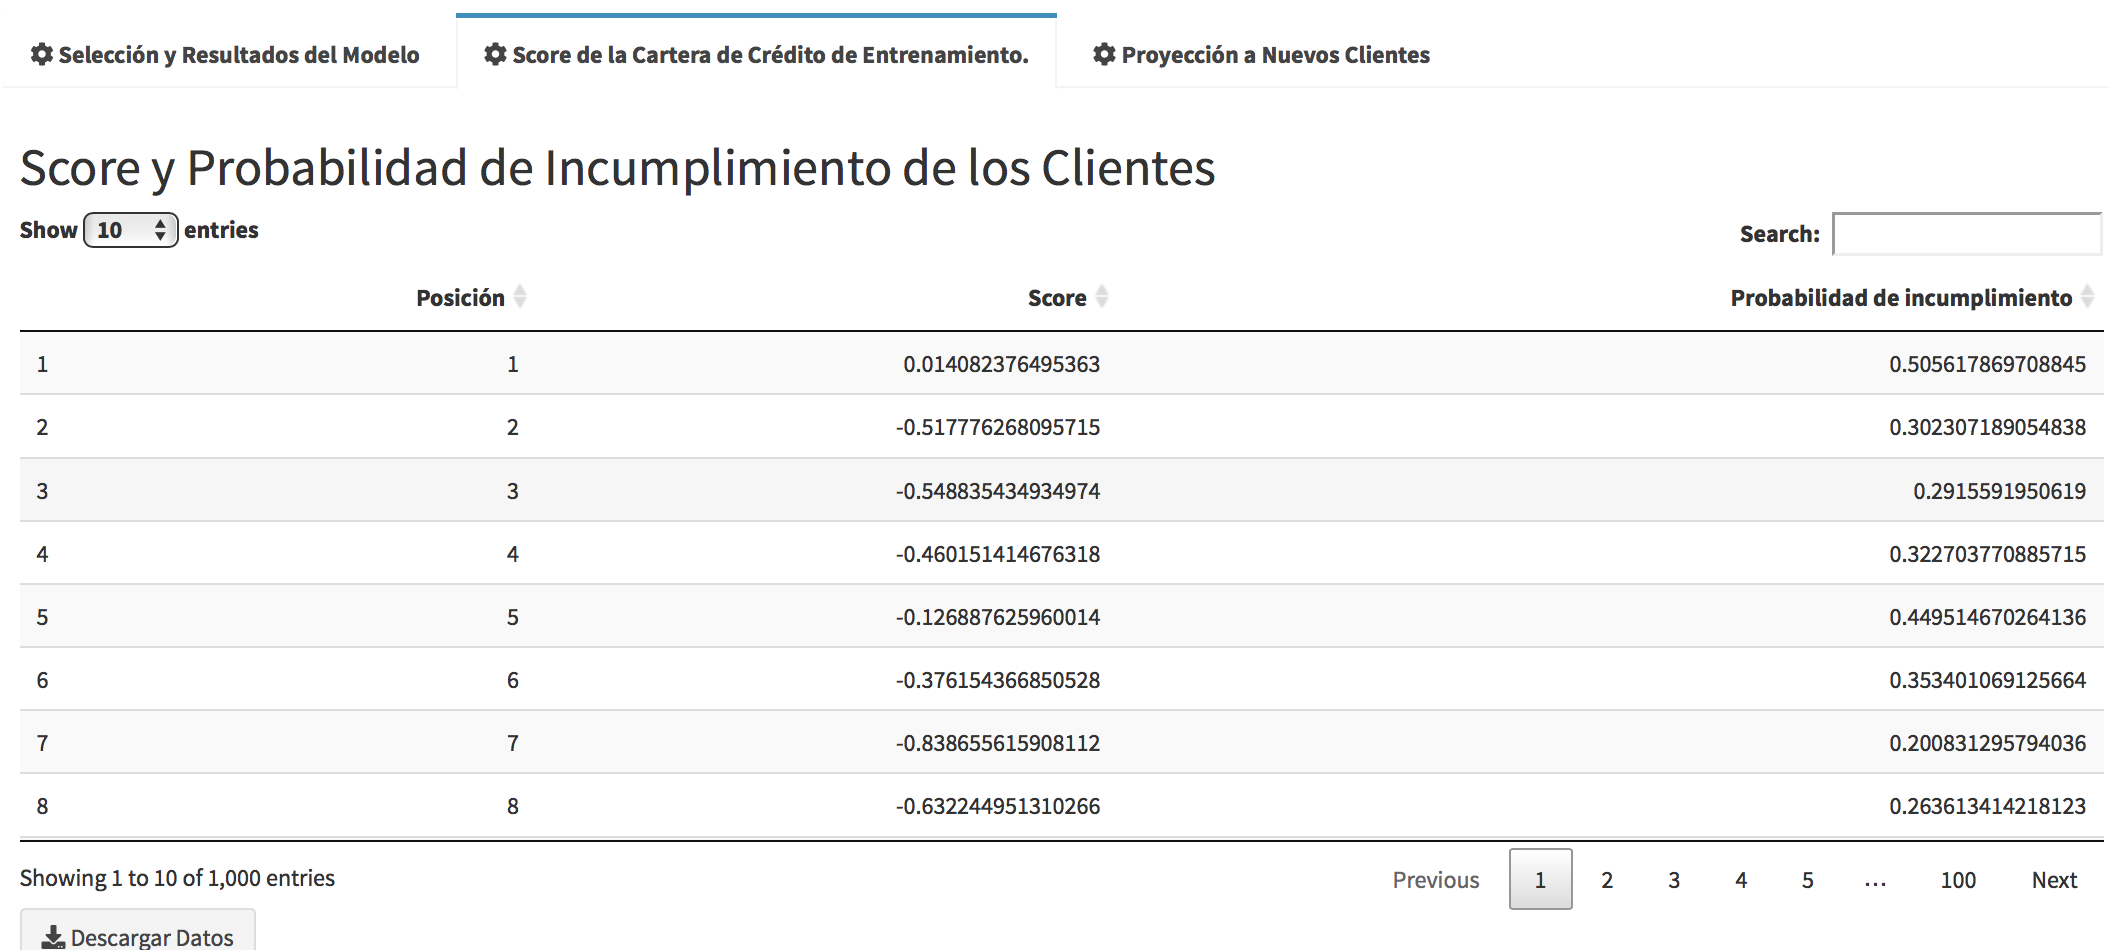
\includegraphics{images/28.png}
\caption{\label{fig:"sd"}}
\end{figure}

\hypertarget{proyeccion-a-nuevos-clientes}{%
\subsubsection{Proyección a nuevos clientes}\label{proyeccion-a-nuevos-clientes}}

En esta sección podemos usar el score para calcular la probabilidad de incumplimiento de nuevos clientes.

\begin{figure}
\centering
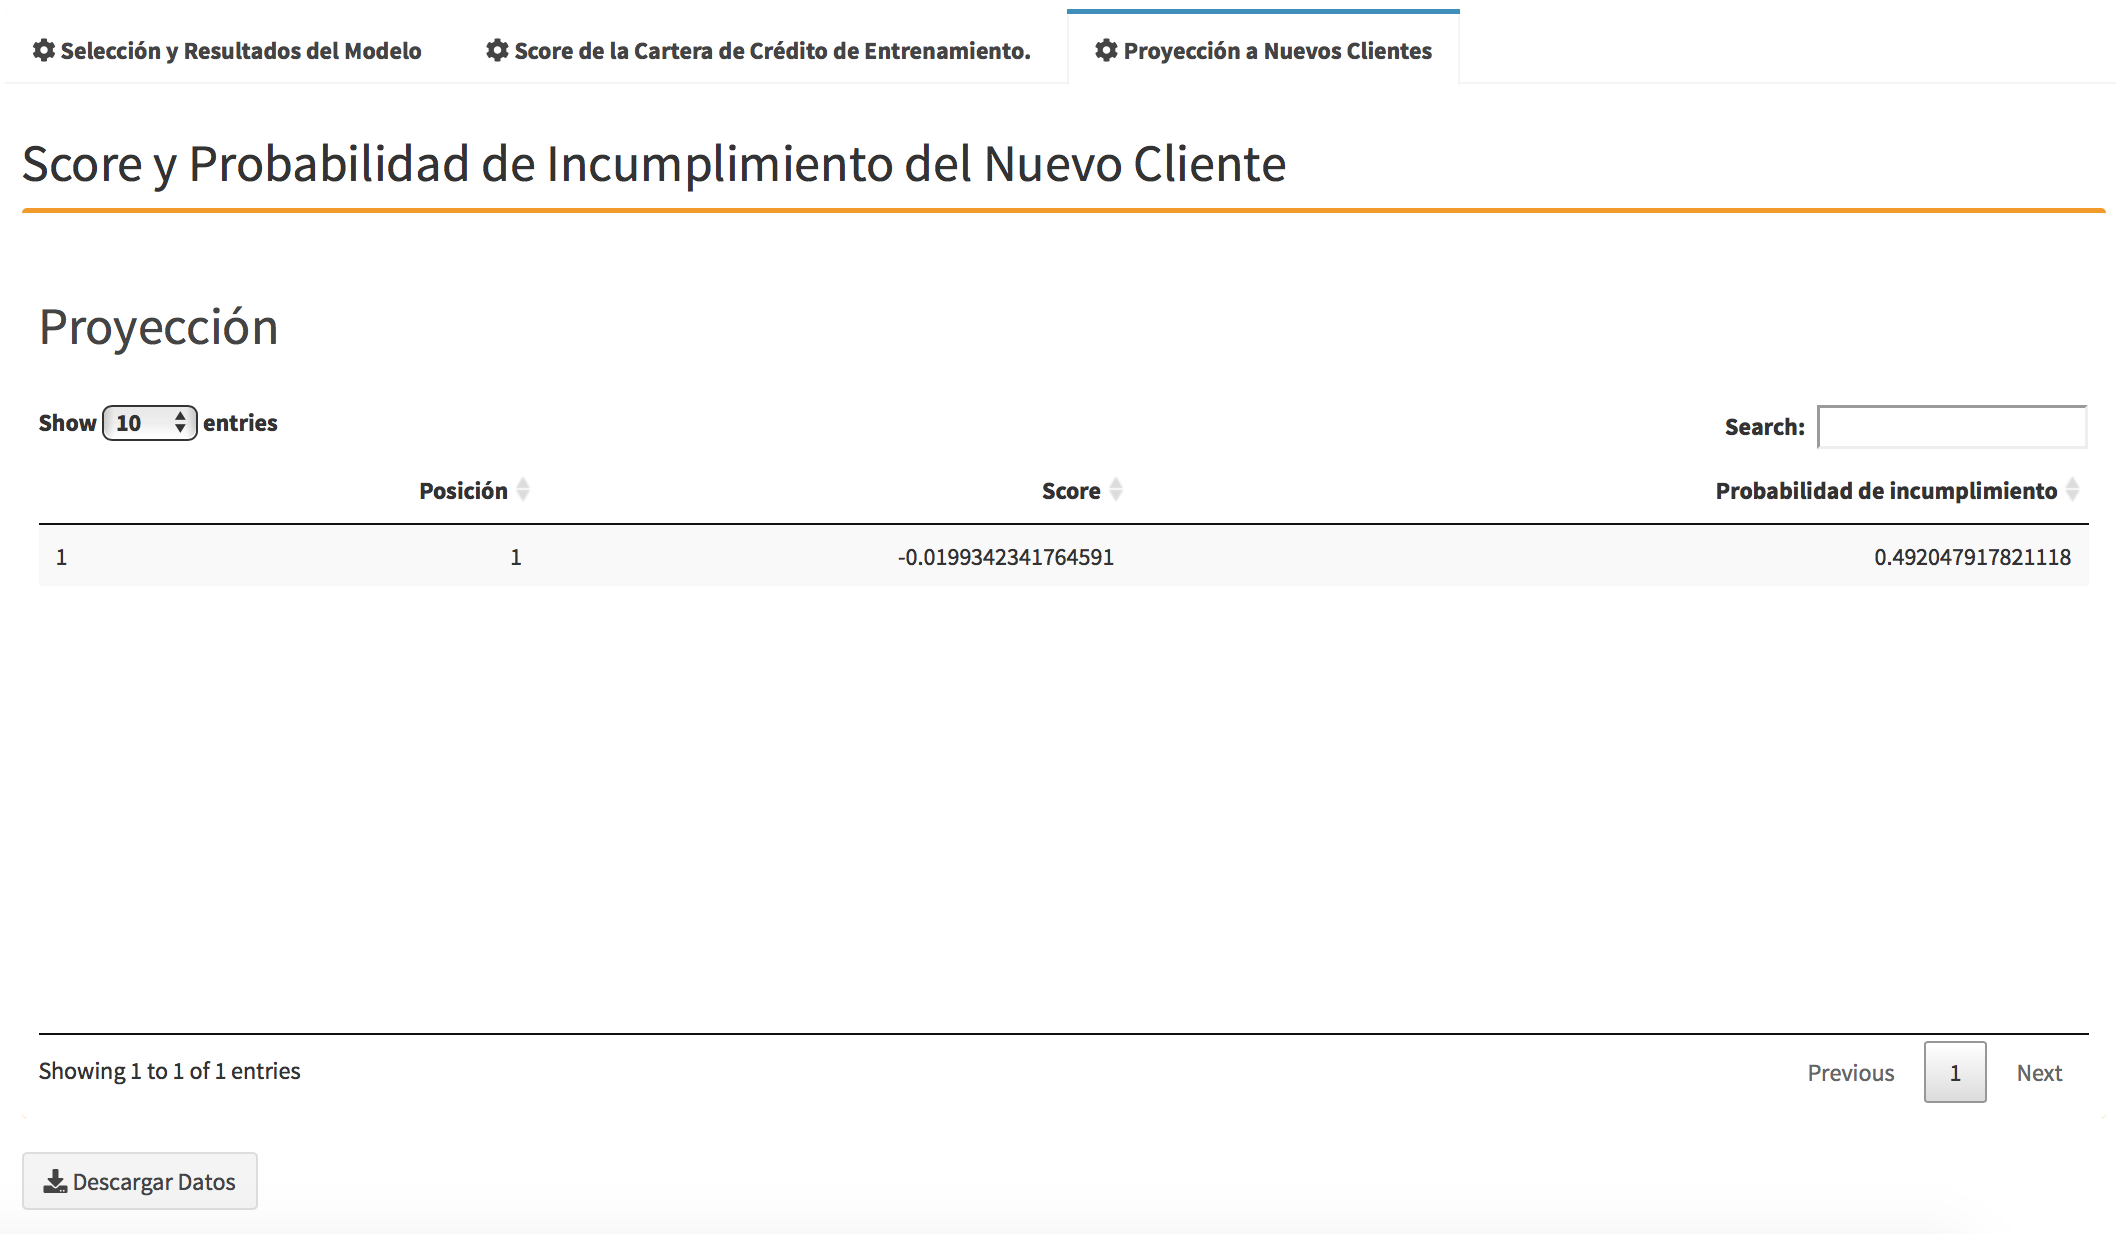
\includegraphics{images/29.png}
\caption{\label{fig:"sd"}}
\end{figure}

\hypertarget{rating-de-credito}{%
\subsection{Rating de Crédito}\label{rating-de-credito}}

En esta sección crearemos el sistema de rating para clasificar a los clientes.

\hypertarget{construccion-del-modelo-de-rating}{%
\subsubsection{Construcción del Modelo de Rating}\label{construccion-del-modelo-de-rating}}

En esta sección se muestra la información estadística del modelo rating usando análisis de discriminante.

\begin{figure}
\centering
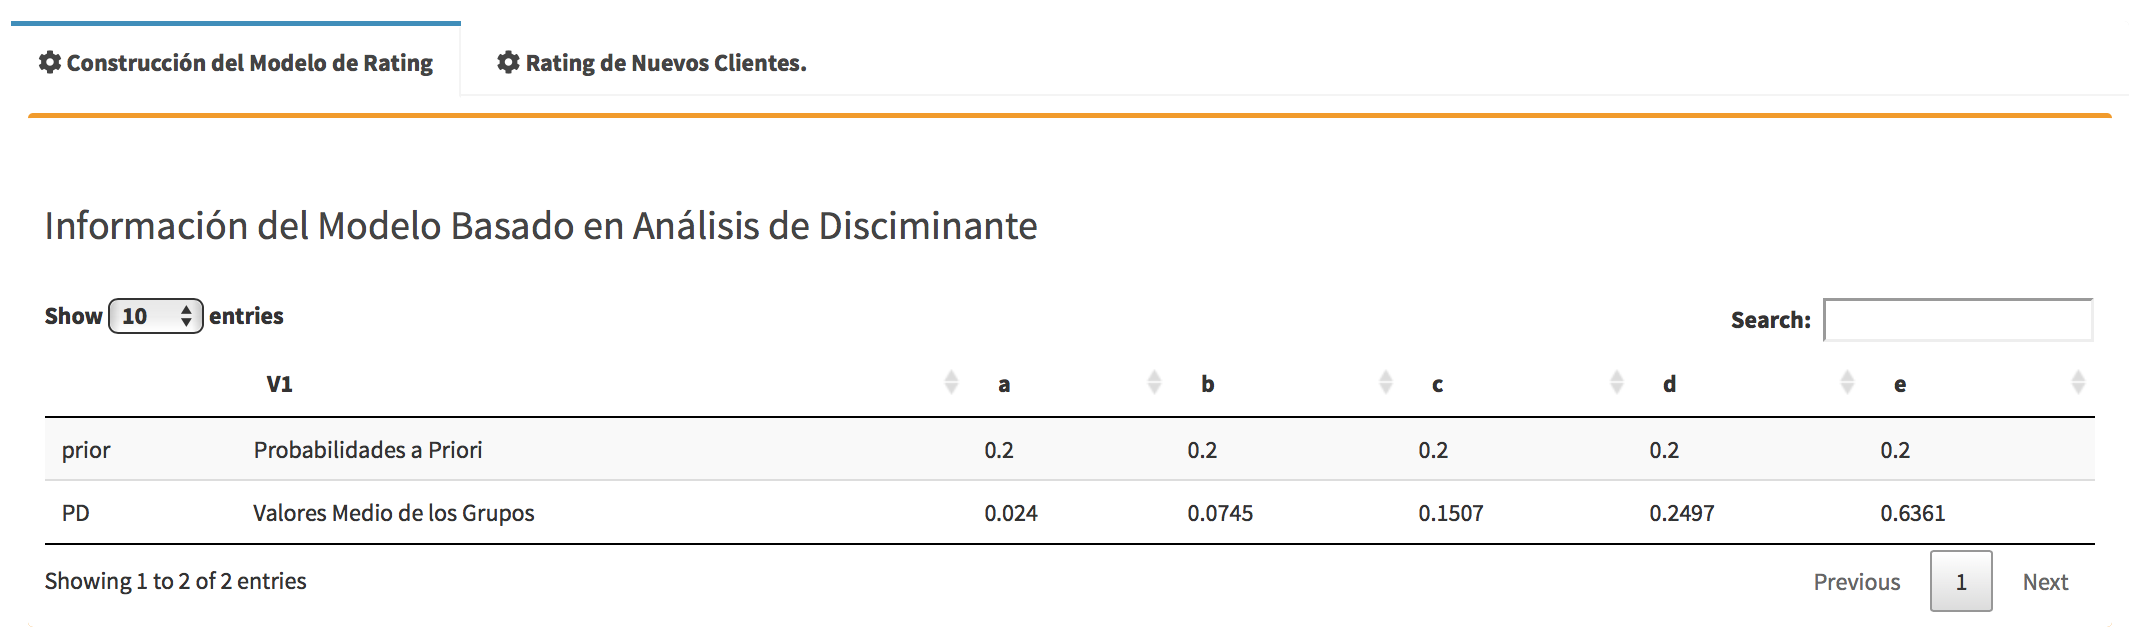
\includegraphics{images/30.png}
\caption{\label{fig:"sd"}}
\end{figure}

\hypertarget{rating-de-nuevos-clientes}{%
\subsubsection{Rating de Nuevos clientes}\label{rating-de-nuevos-clientes}}

Una vez creado el modelo de rating en esta sección se muestra la proyección a nuevos clientes.

\begin{figure}
\centering
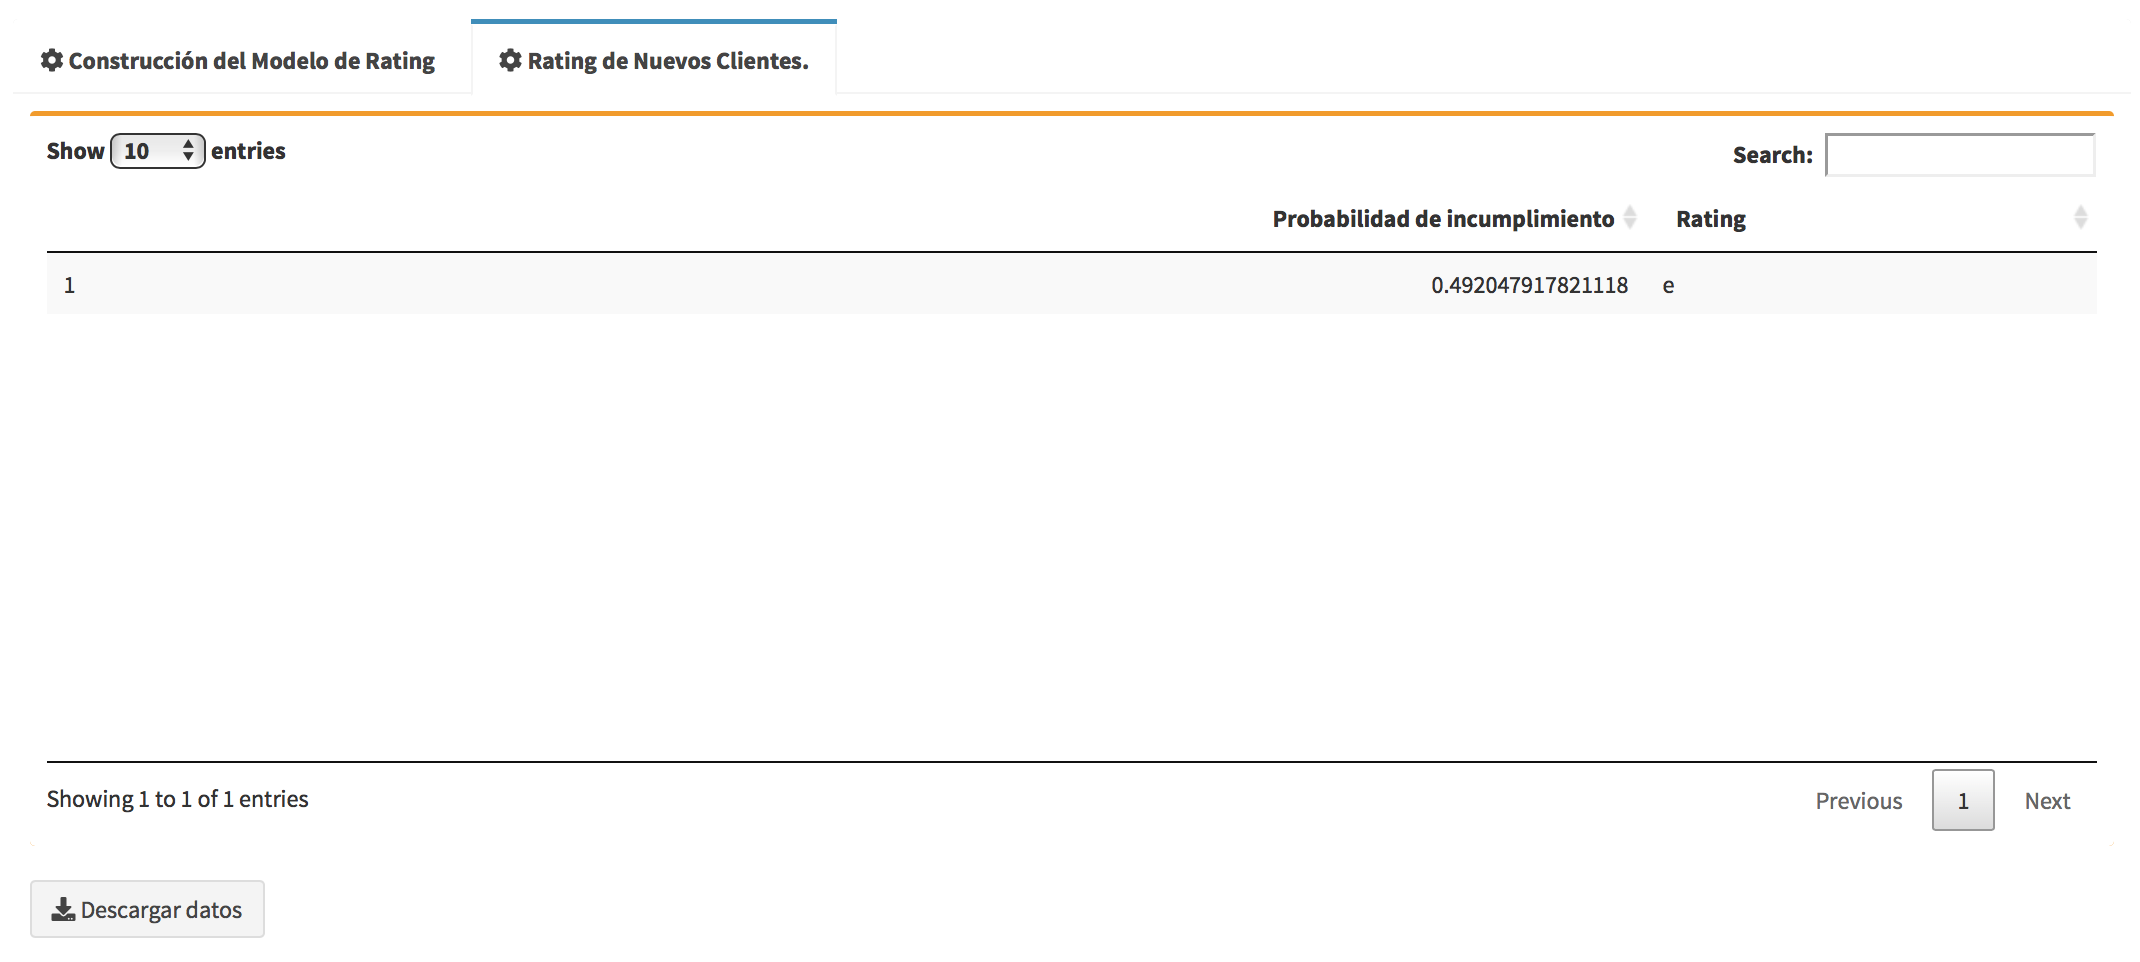
\includegraphics{images/31.png}
\caption{\label{fig:"sd"}}
\end{figure}

\hypertarget{perdida-por-incumplimiento-1}{%
\section{Pérdida por incumplimiento}\label{perdida-por-incumplimiento-1}}

En esta sección calcularemos las pérdidas esperadas por cliente, tendremos dos opciones: pérdida de la cartera en general y pérdida por clasificación.

\begin{figure}
\centering
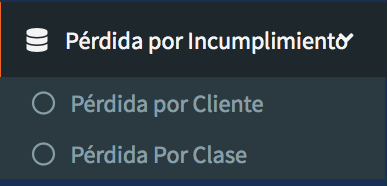
\includegraphics{images/32.png}
\caption{\label{fig:"sd"}}
\end{figure}

\hypertarget{perdida-por-cliente}{%
\subsection{Pérdida por Cliente}\label{perdida-por-cliente}}

\hypertarget{datos}{%
\subsubsection{Datos}\label{datos}}

En esta sección veremos un histograma de las pérdidas históricas

\begin{figure}
\centering
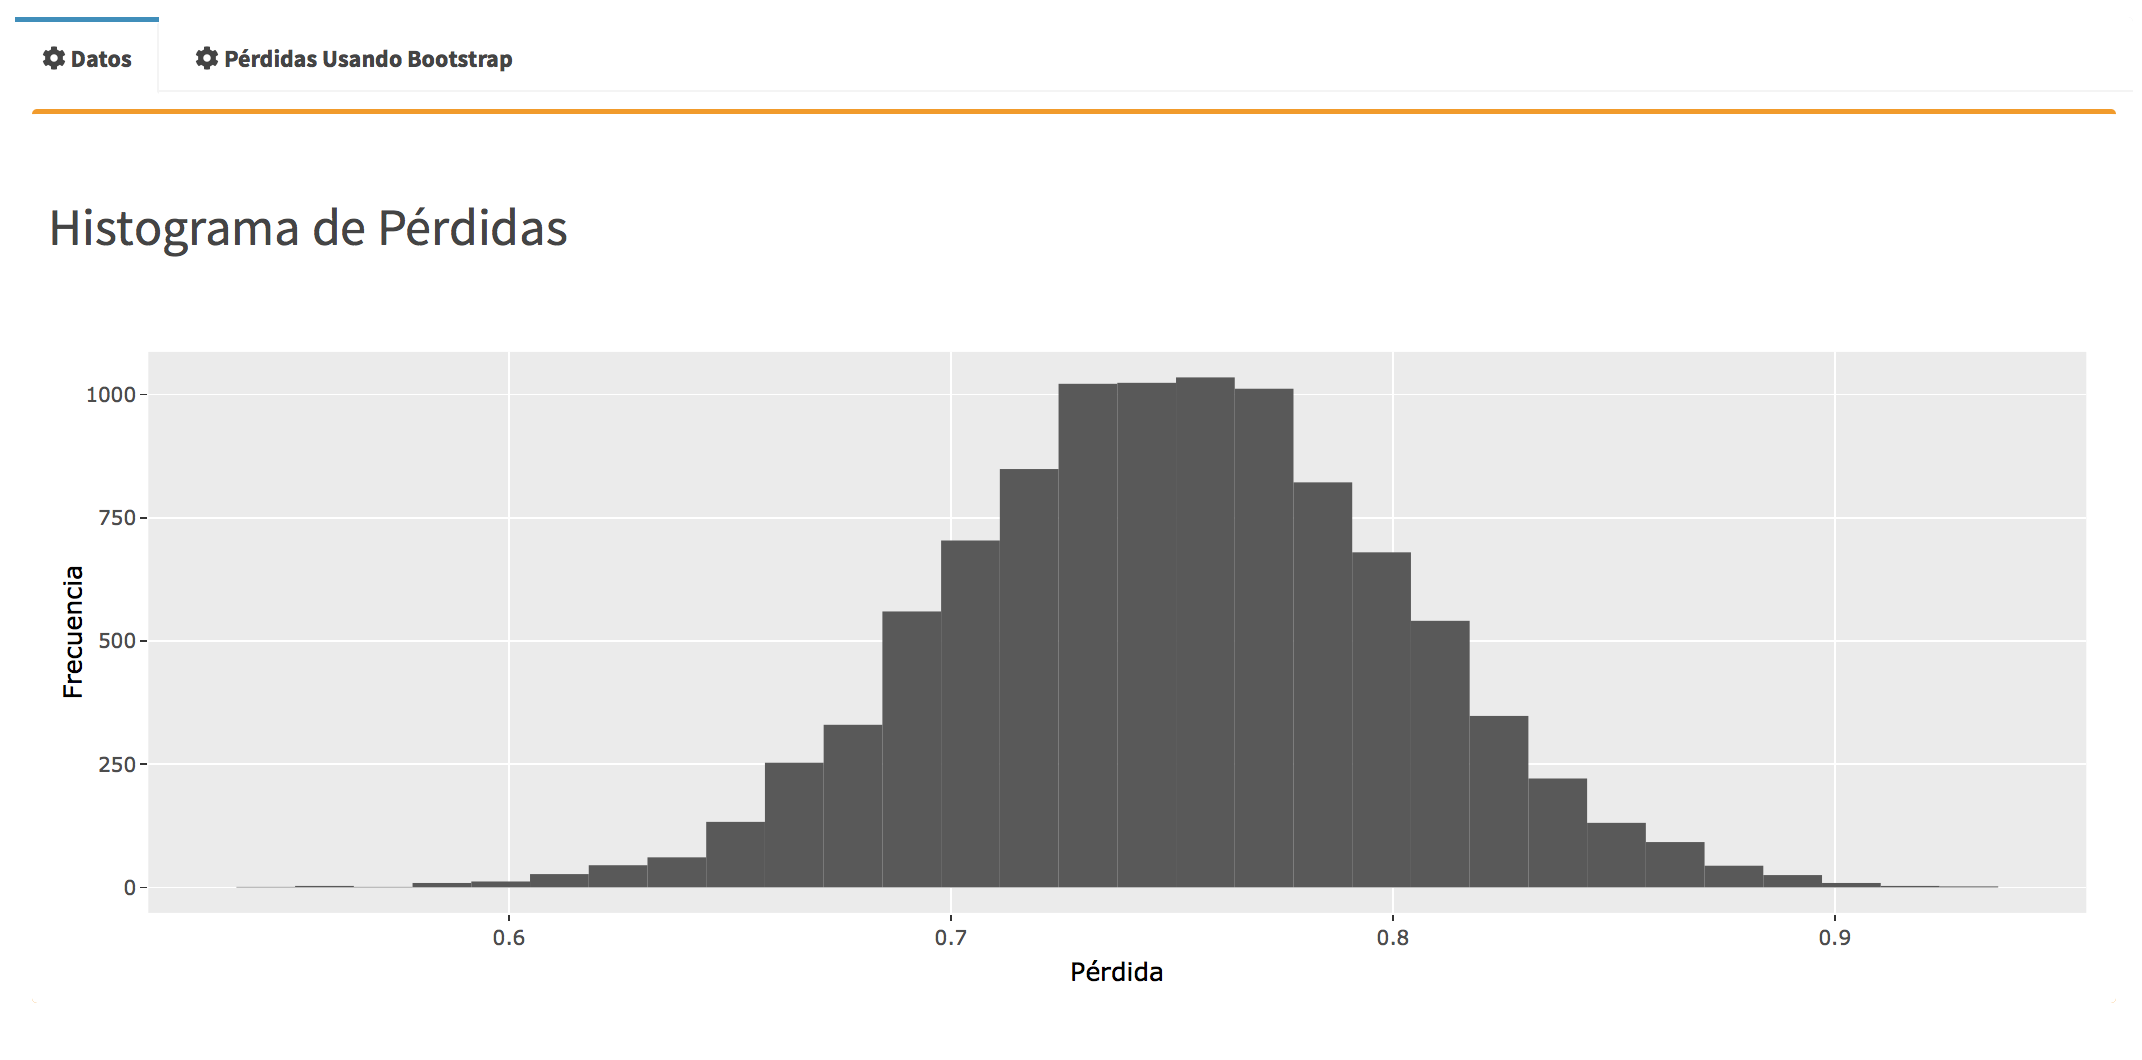
\includegraphics{images/33.png}
\caption{\label{fig:"sd"}}
\end{figure}

\hypertarget{perdidas-usando-bootstrap}{%
\subsubsection{Pérdidas usando bootstrap}\label{perdidas-usando-bootstrap}}

La técnica bootstrap consiste en simular usando la data muchas submuestras, para obtener estadísticos fáciles de calcular, tendremos dos opciones para iniciar la simulación: Número de sub-muestras y Tamaños de las sub-muestras

\begin{figure}
\centering
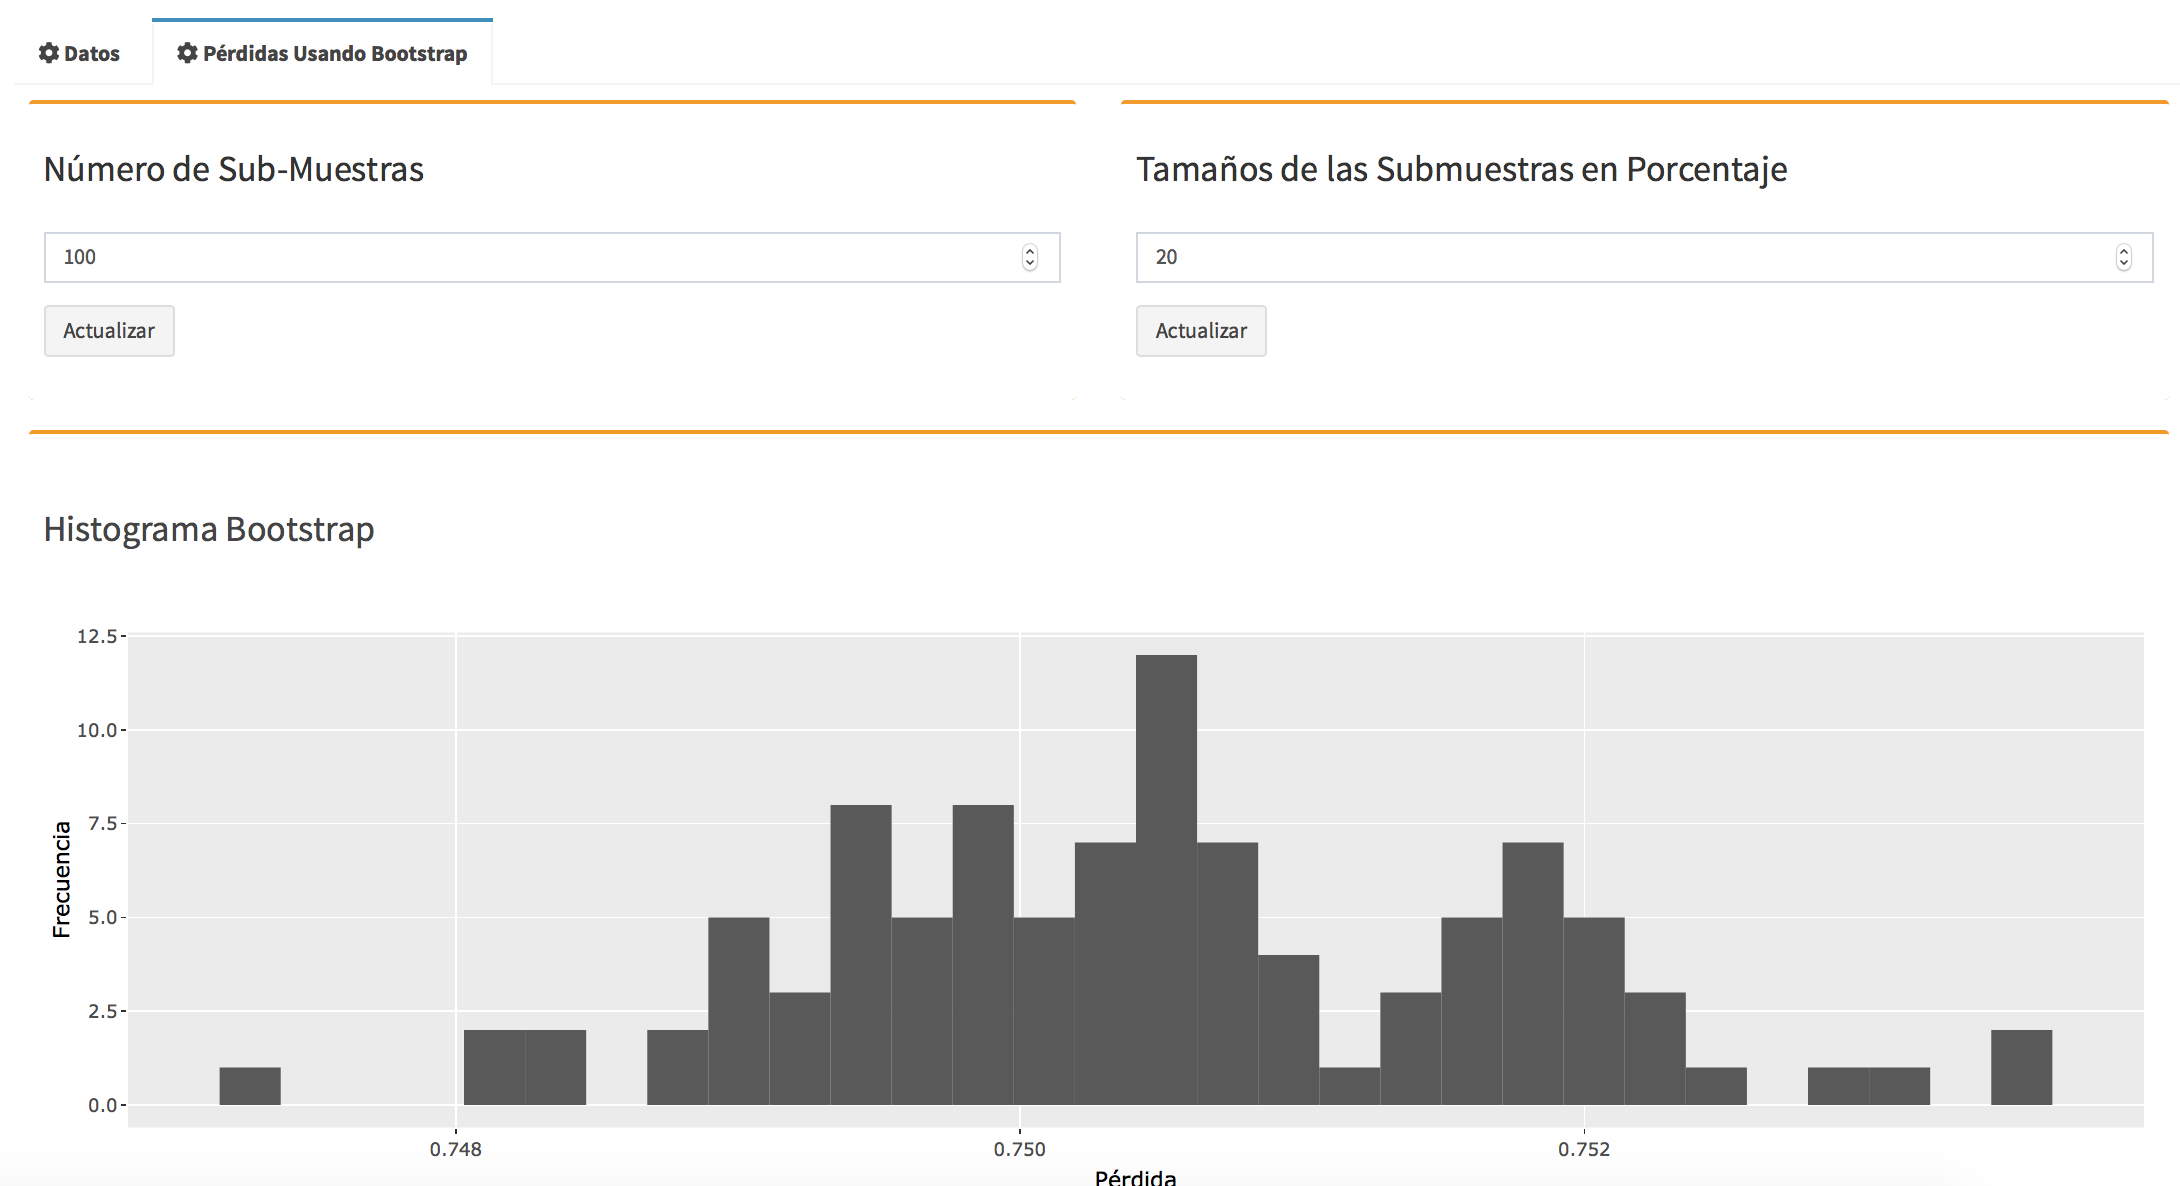
\includegraphics{images/34.png}
\caption{\label{fig:"sd"}}
\end{figure}

\hypertarget{perdida-por-clases}{%
\subsection{Pérdida por Clases}\label{perdida-por-clases}}

\hypertarget{perdidas-promedios}{%
\subsubsection{Pérdidas Promedios}\label{perdidas-promedios}}

En esta sección se calculan las pérdidas promedios por clase o categoría.

\begin{figure}
\centering
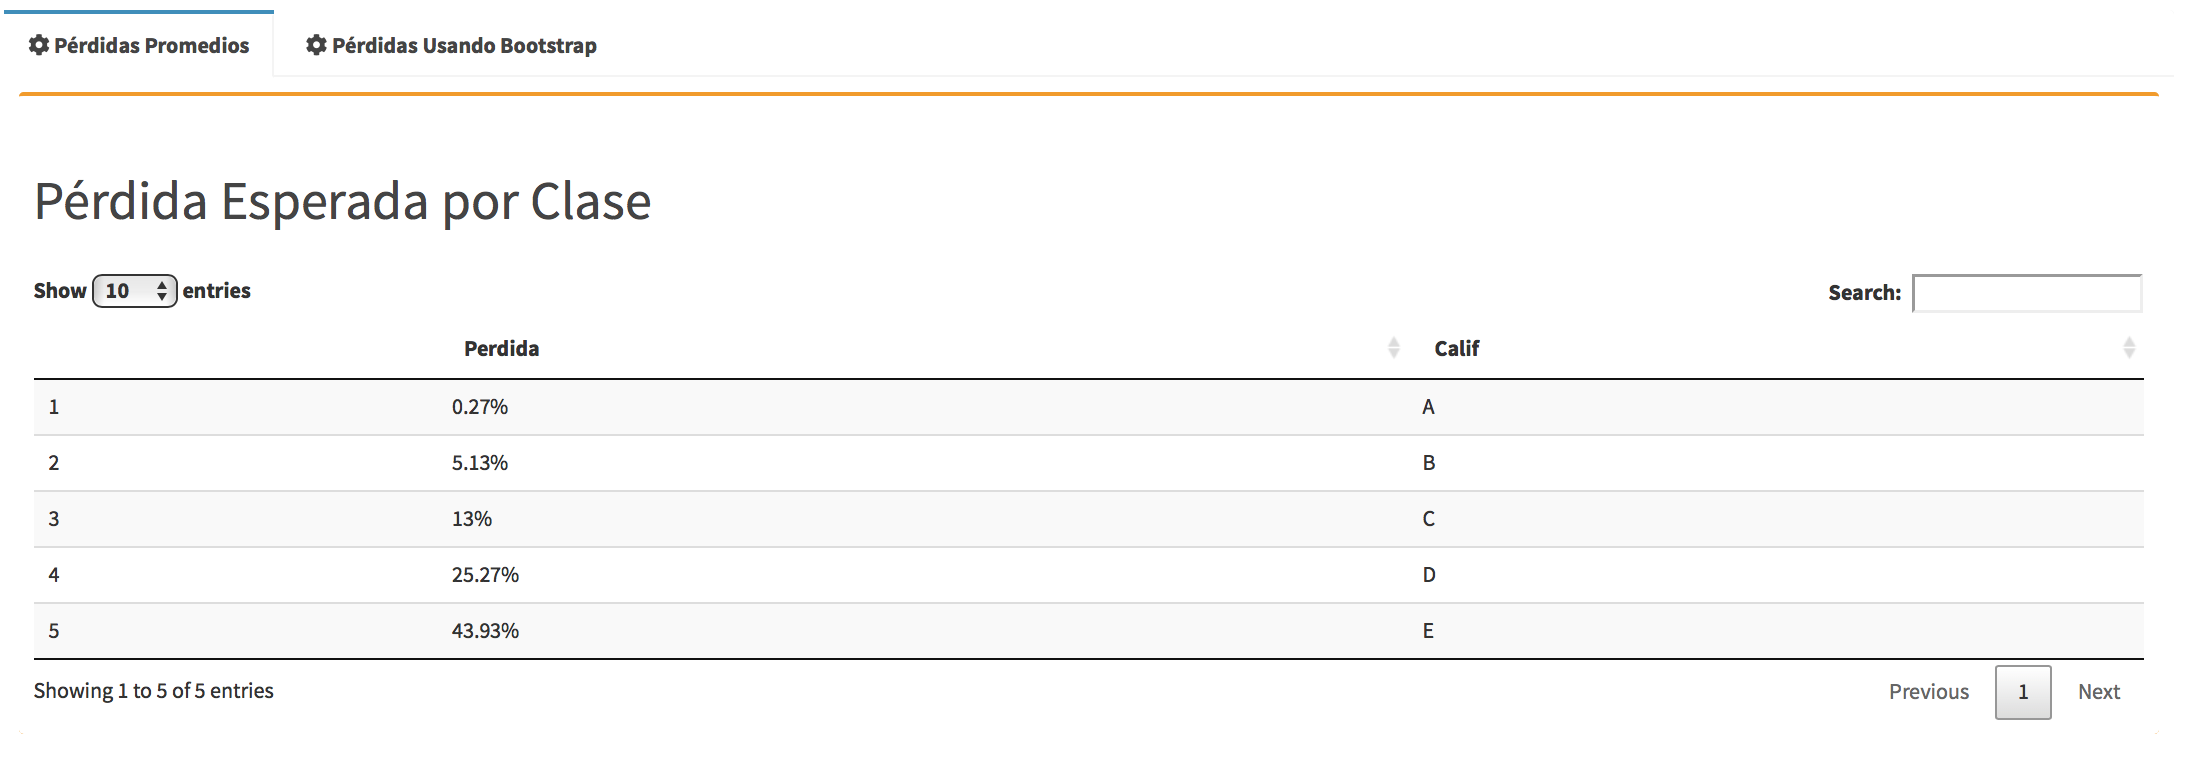
\includegraphics{images/35.png}
\caption{\label{fig:"sd"}}
\end{figure}

\hypertarget{perdidas-usando-bootstrap-1}{%
\subsubsection{Pérdidas usando bootstrap}\label{perdidas-usando-bootstrap-1}}

De igual manera se usa bootstrap, pero en este caso se usa por categoría.

\begin{figure}
\centering
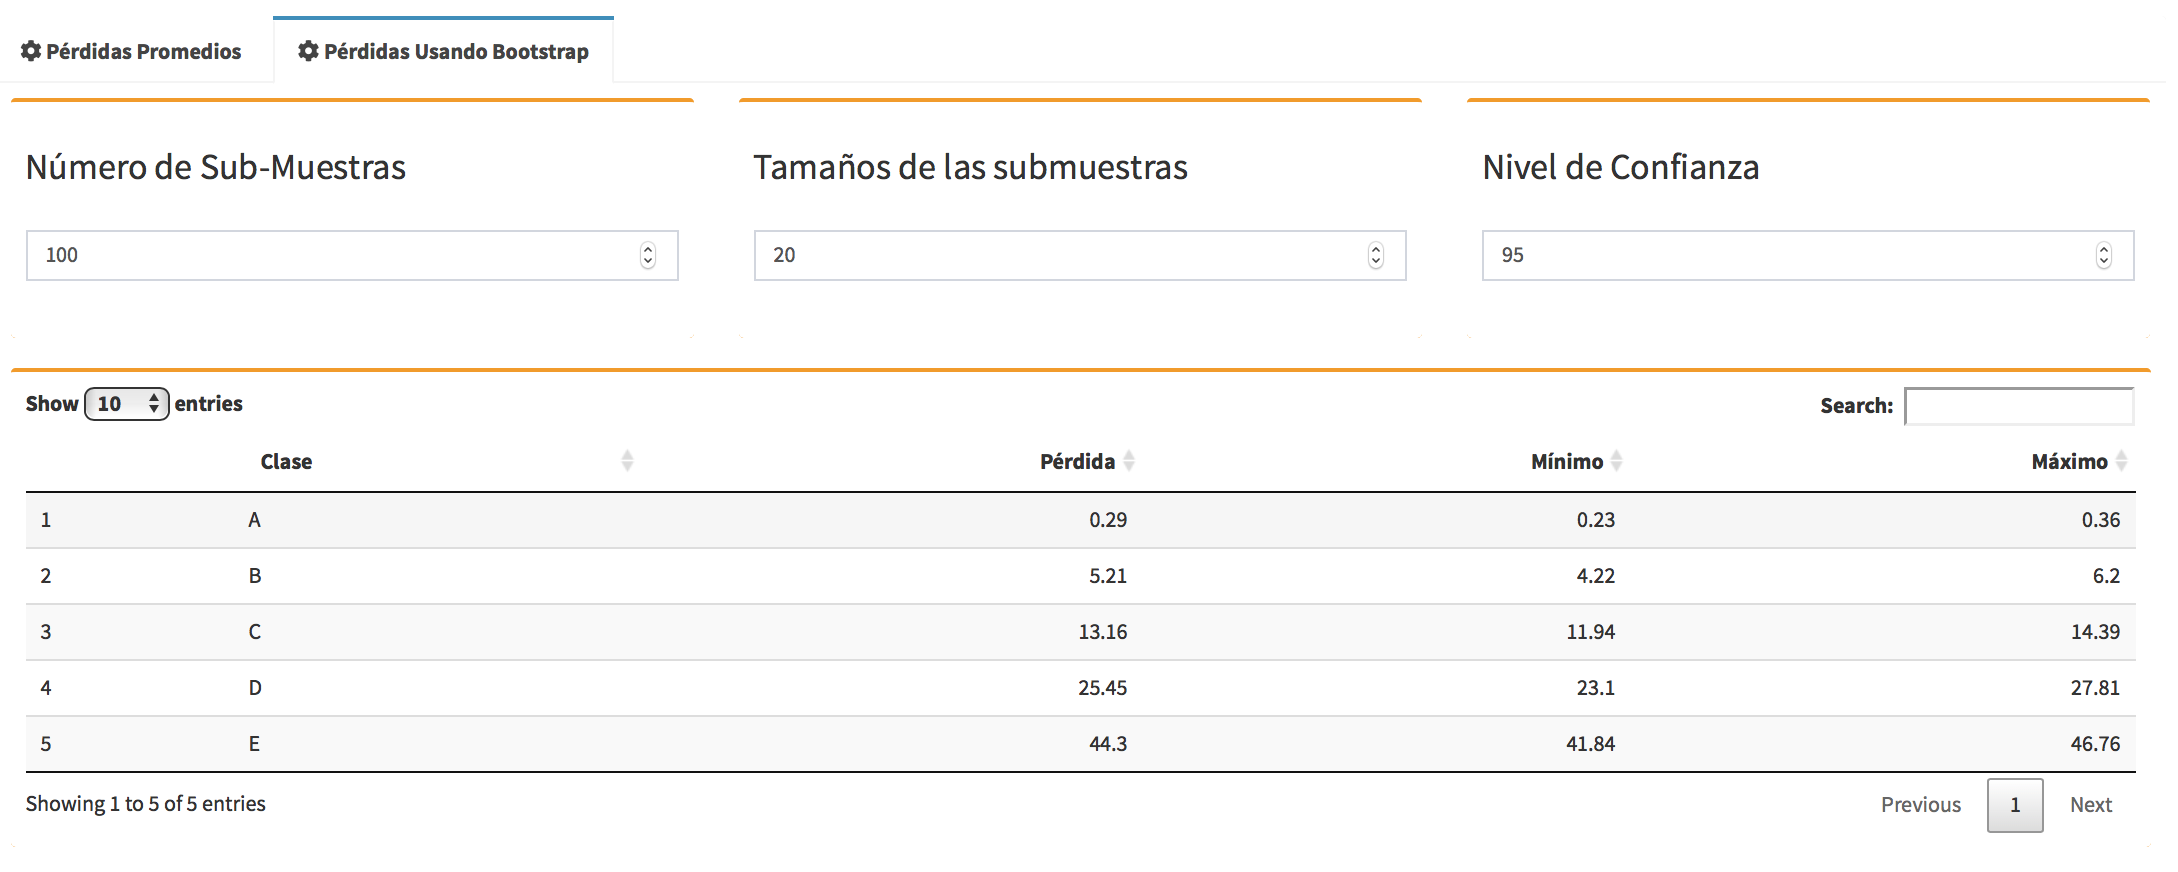
\includegraphics{images/36.png}
\caption{\label{fig:"sd"}}
\end{figure}

\hypertarget{matriz-de-trnasicion}{%
\section{Matriz de trnasición}\label{matriz-de-trnasicion}}

En esta sección se calcula la matriz de transición crediticia.

\begin{figure}
\centering

\includegraphics{images/37.png}
\caption{\label{fig:"sd"}}
\end{figure}

\hypertarget{matriz-de-transicion-3}{%
\subsection{Matriz de transición}\label{matriz-de-transicion-3}}

Una vez cargados los datos, se calcula la matriz de transición, usando tasas ponderadas históricas.

\begin{figure}
\centering
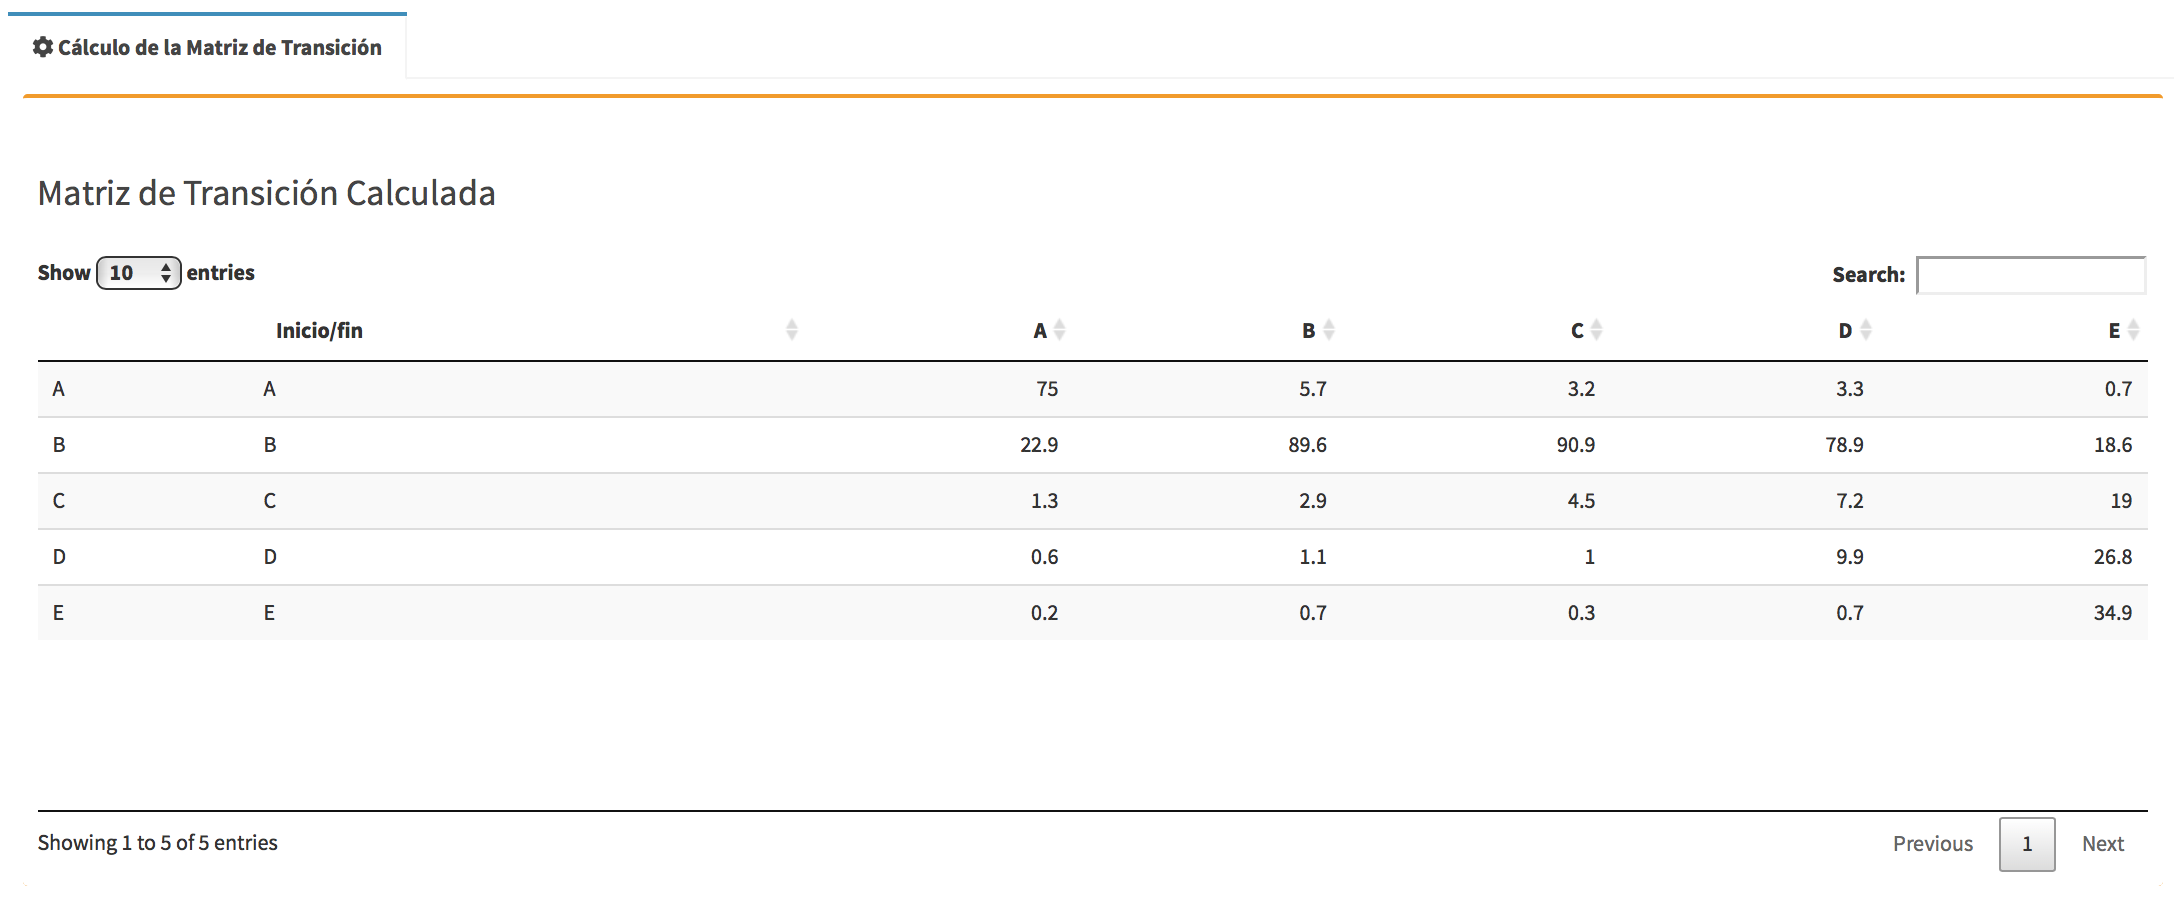
\includegraphics{images/38.png}
\caption{\label{fig:"sd"}}
\end{figure}

\hypertarget{creditrisk-2}{%
\section{CreditRisk+}\label{creditrisk-2}}

Ene sta sección se mostraron los resultados de usar la metodología de riesgo de crédito CreditRisk+, la cual está conformada por dos pestañas.

\begin{figure}
\centering
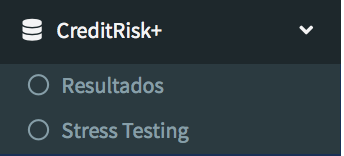
\includegraphics{images/39.png}
\caption{\label{fig:"sd"}}
\end{figure}

\hypertarget{resultados}{%
\subsection{Resultados}\label{resultados}}

En esta sección se mostrarán los resultados correspondiente a la metodología

\hypertarget{perdida-esperada-por-cliente}{%
\subsubsection{Pérdida esperada por cliente}\label{perdida-esperada-por-cliente}}

En esta sección se muestra una tabla estadística de la información sobre la pérdida de los clientes.

\begin{figure}
\centering
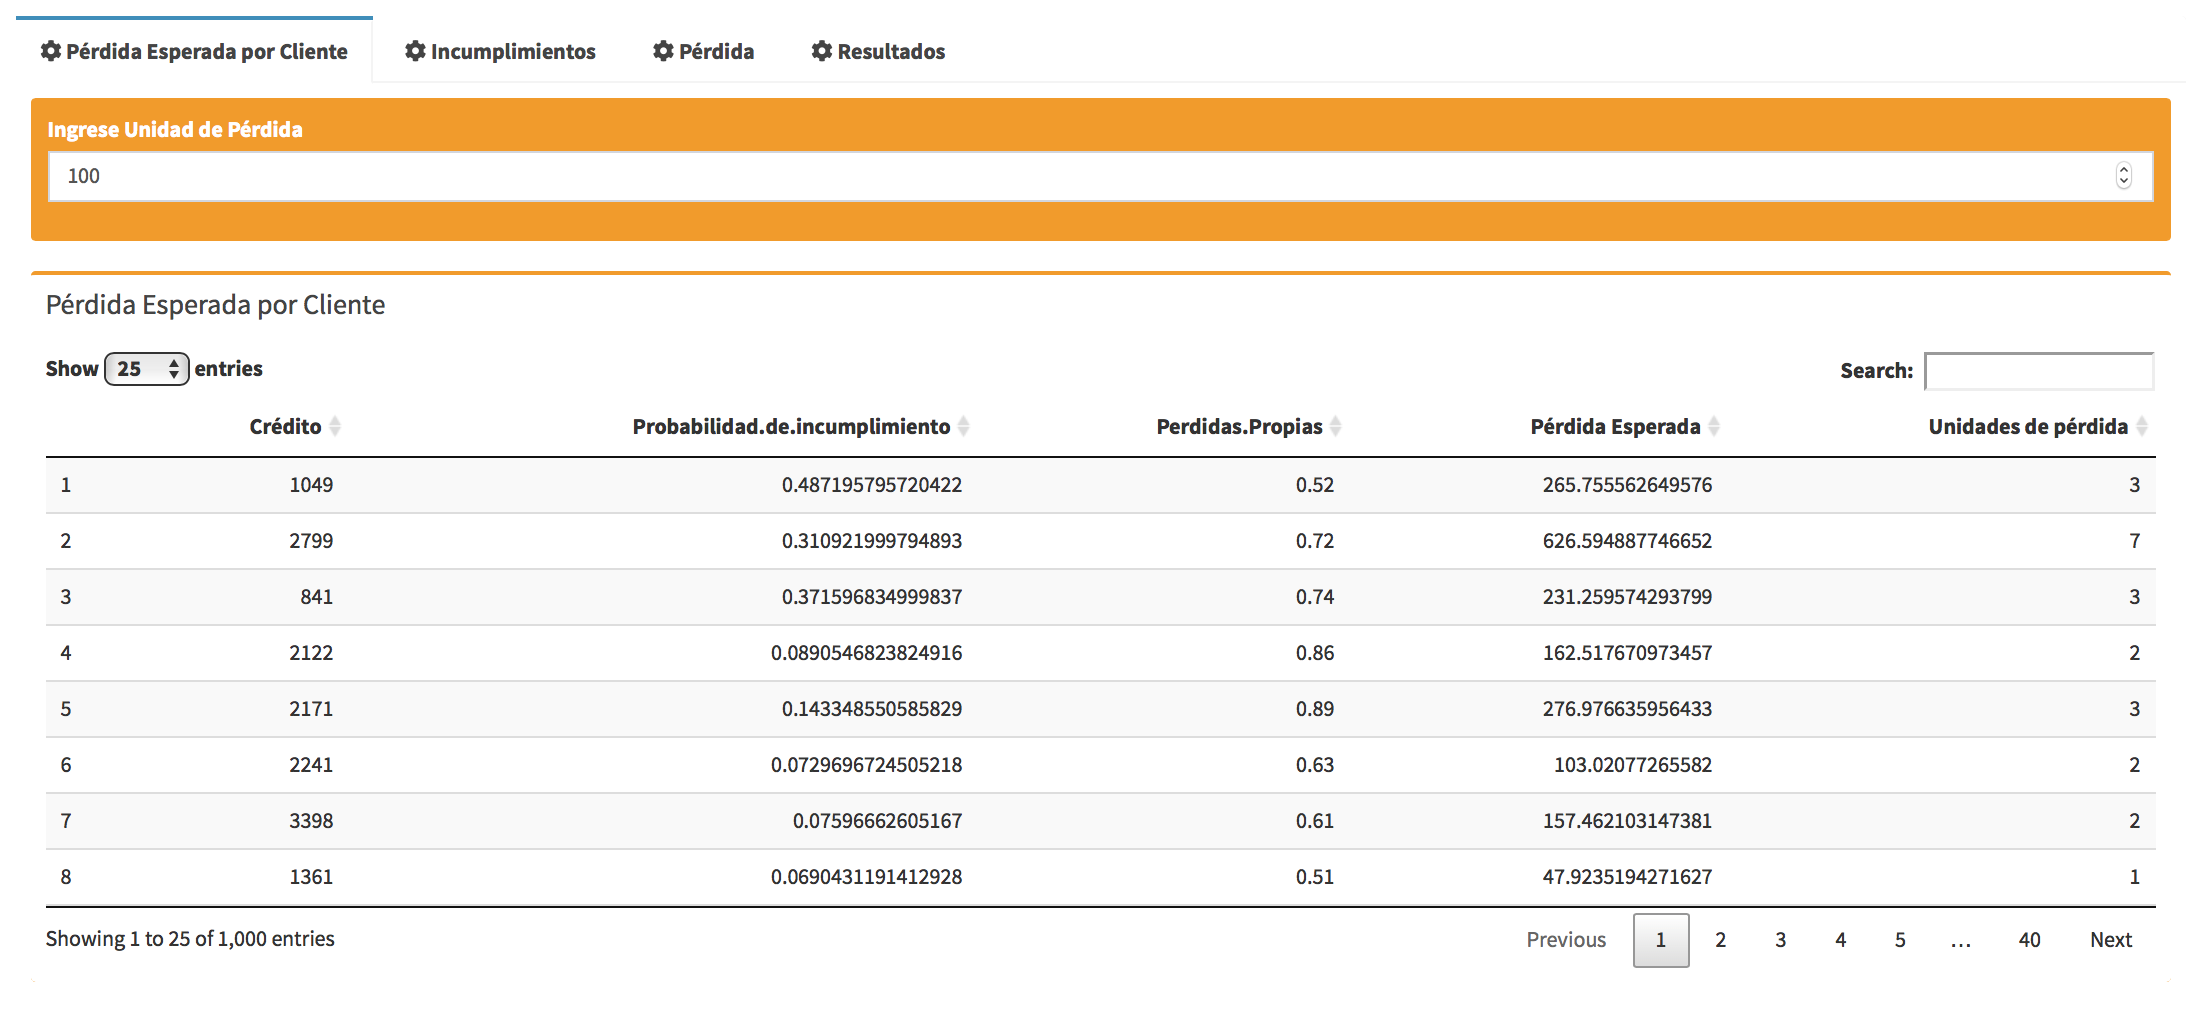
\includegraphics{images/40.png}
\caption{\label{fig:"sd"}}
\end{figure}

\hypertarget{incumplimientos}{%
\subsubsection{Incumplimientos}\label{incumplimientos}}

En esta sección se muestra la probabilidad de que ocurran \(n\) incumplimientos en la cartera de clientes

\begin{figure}
\centering
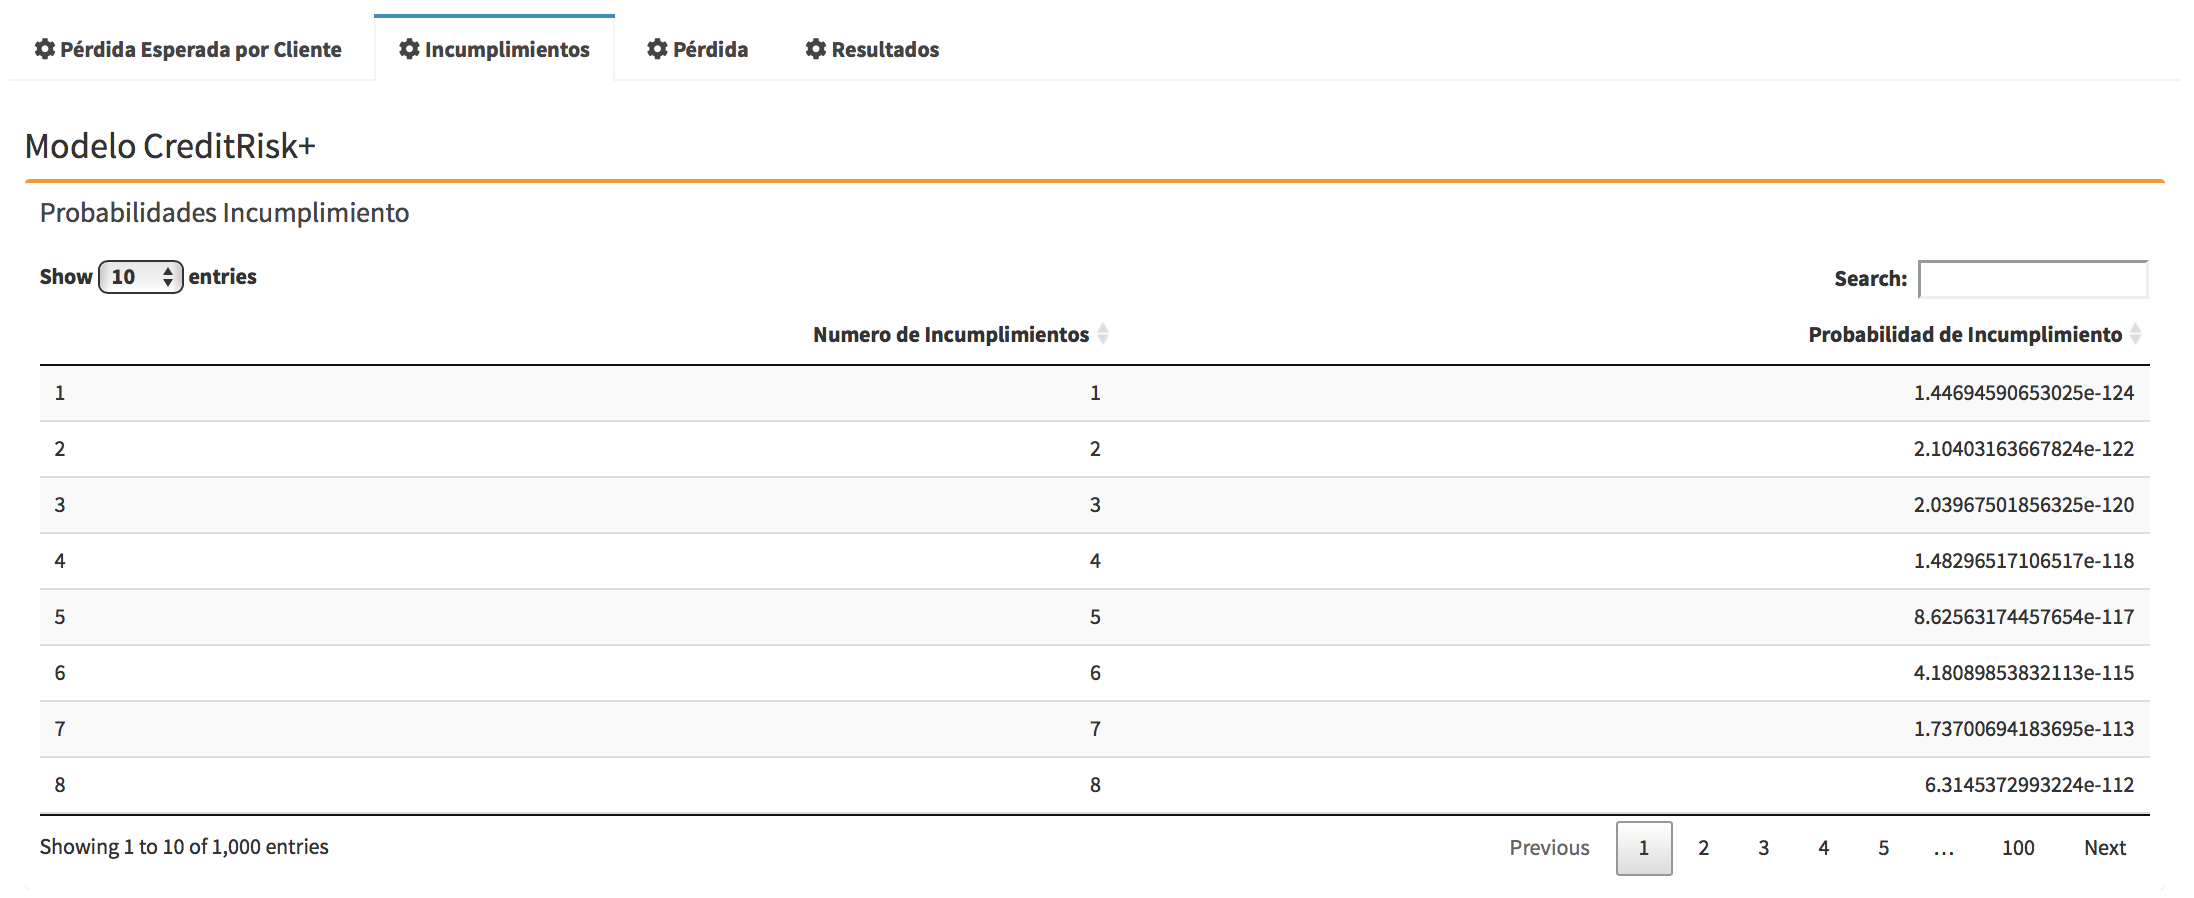
\includegraphics{images/41.png}
\caption{\label{fig:"sd"}}
\end{figure}

Luego se presenta la distribución acumulada del número de incumplimientos

\begin{figure}
\centering
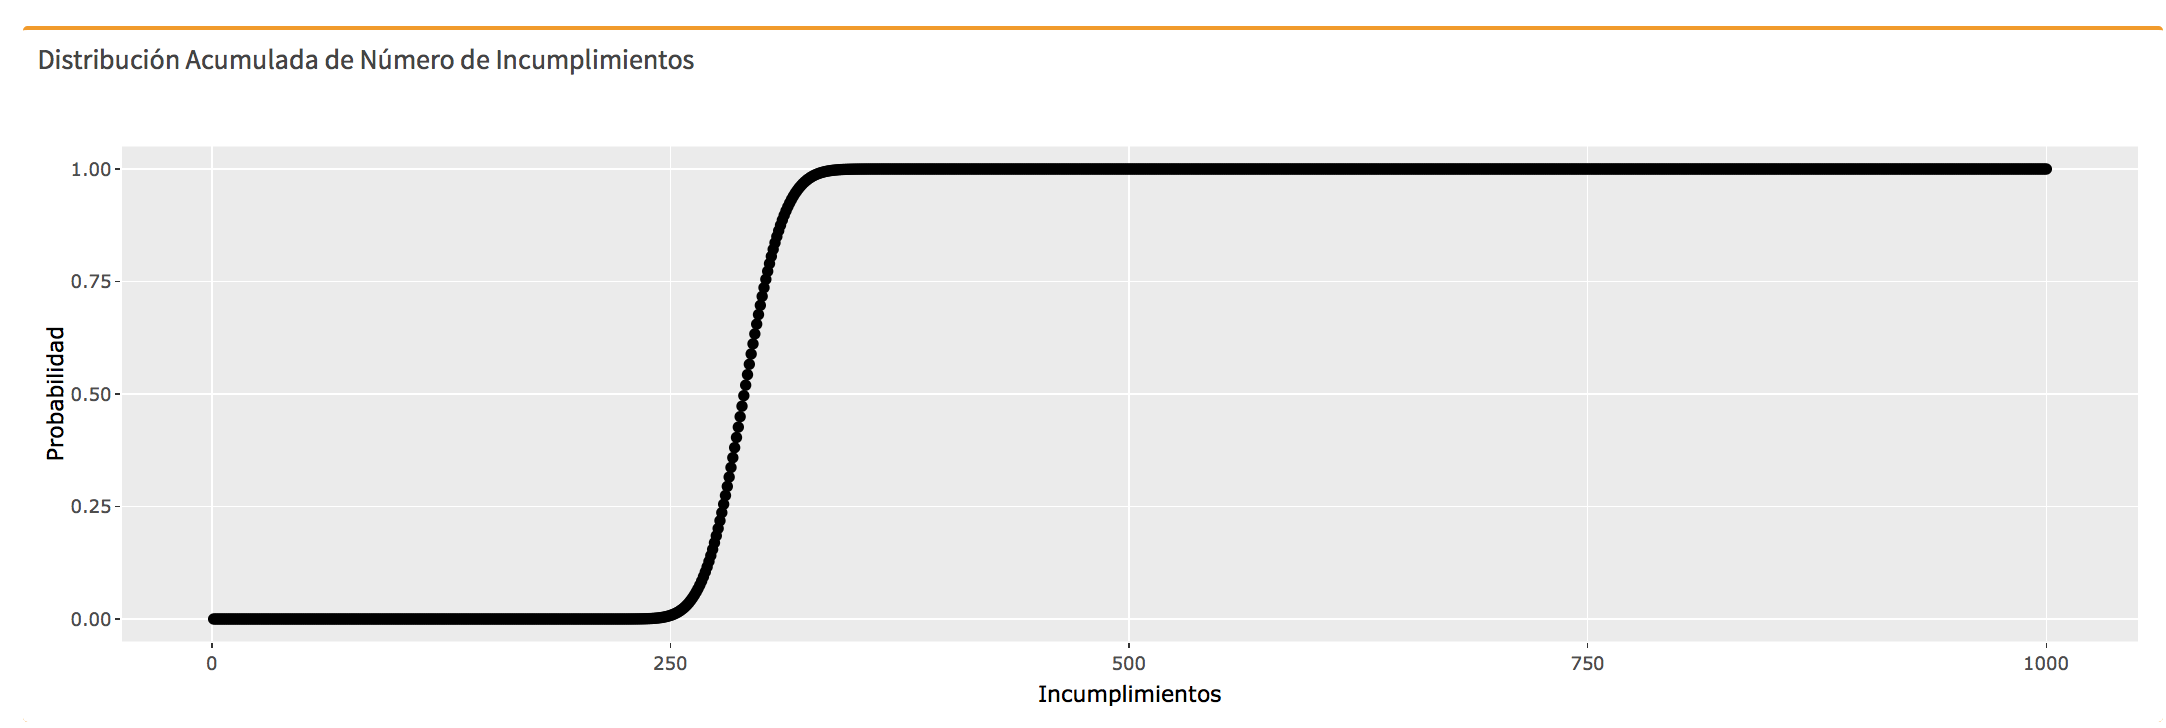
\includegraphics{images/42.png}
\caption{\label{fig:"sd"}}
\end{figure}

\hypertarget{perdida}{%
\subsubsection{Pérdida}\label{perdida}}

En esta sección se muestra la probabilidad de perder \(n\) unidades de pérdida

\begin{figure}
\centering
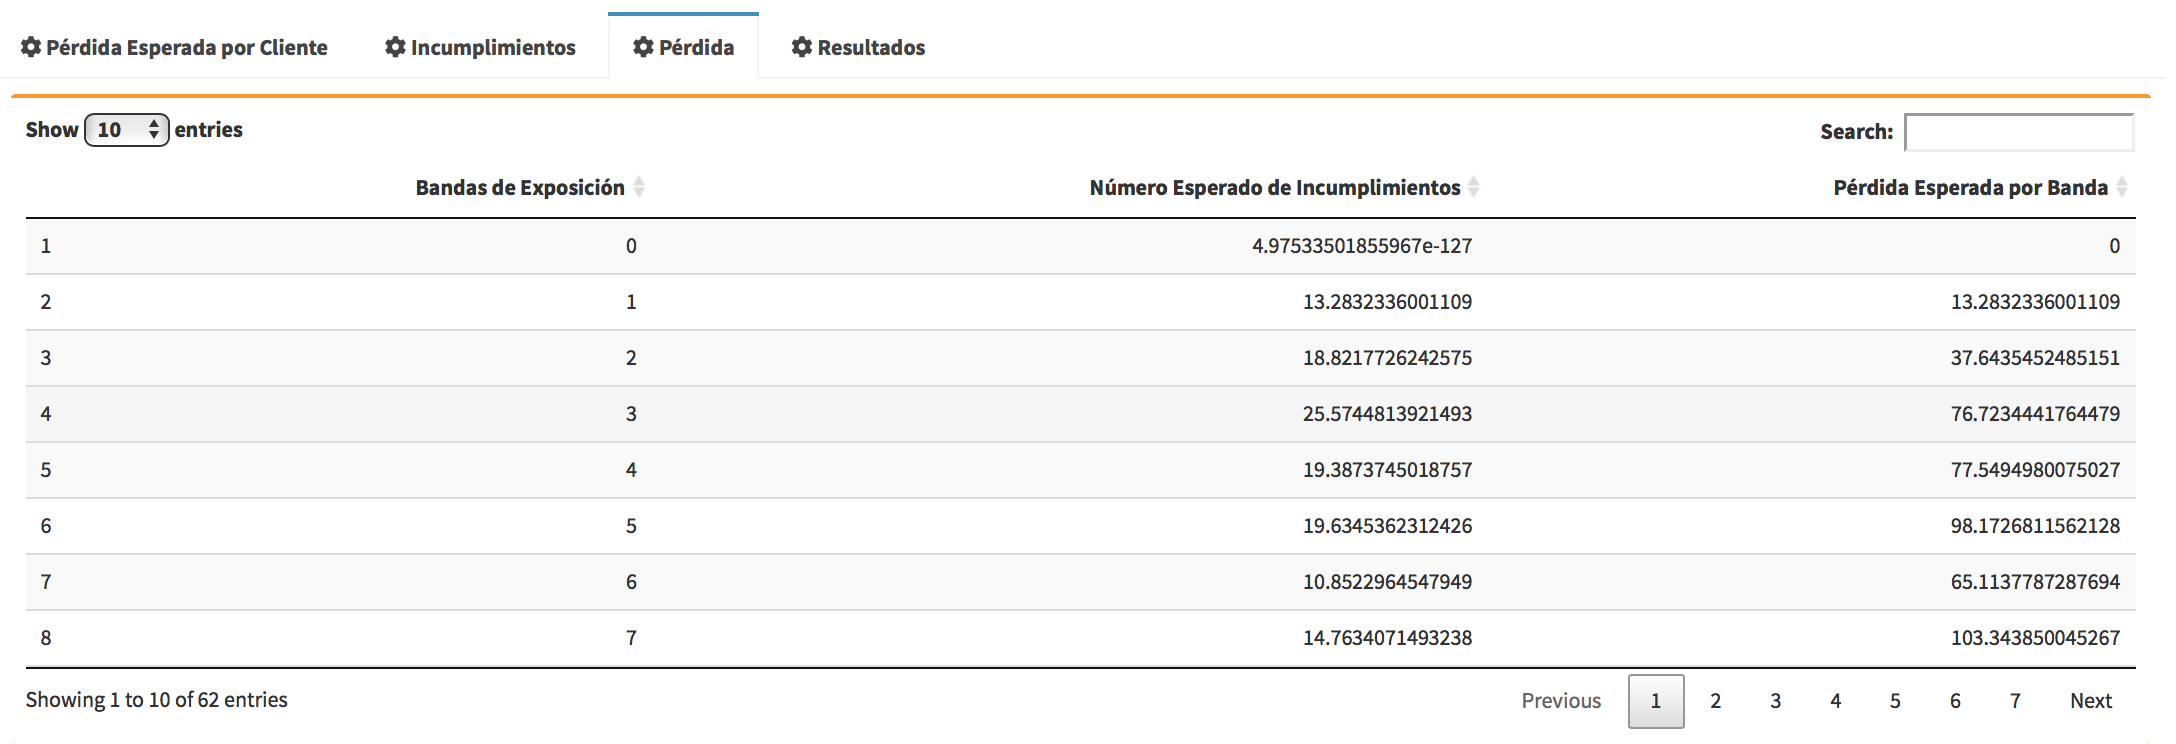
\includegraphics{images/43.png}
\caption{\label{fig:"sd"}}
\end{figure}

Luego se presenta la función de distribución de las pérdidas.

\begin{figure}
\centering
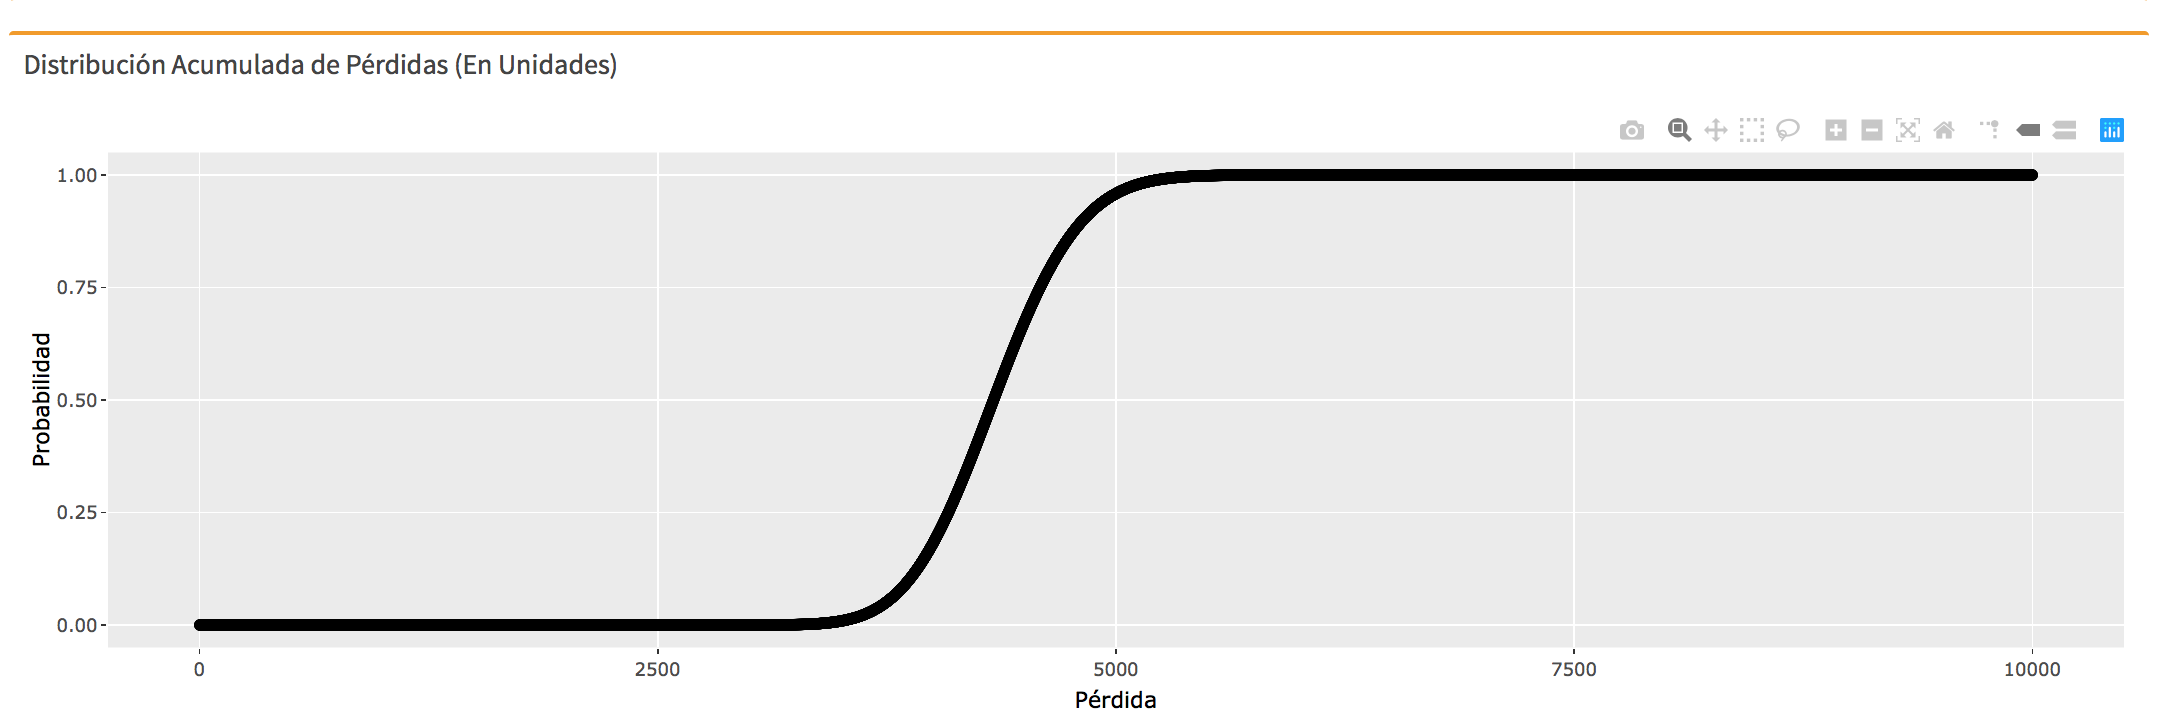
\includegraphics{images/44.png}
\caption{\label{fig:"sd"}}
\end{figure}

\hypertarget{resultados-1}{%
\subsubsection{Resultados}\label{resultados-1}}

En esta sección se muestran las métricas de riesgo de la metodología.

\begin{figure}
\centering
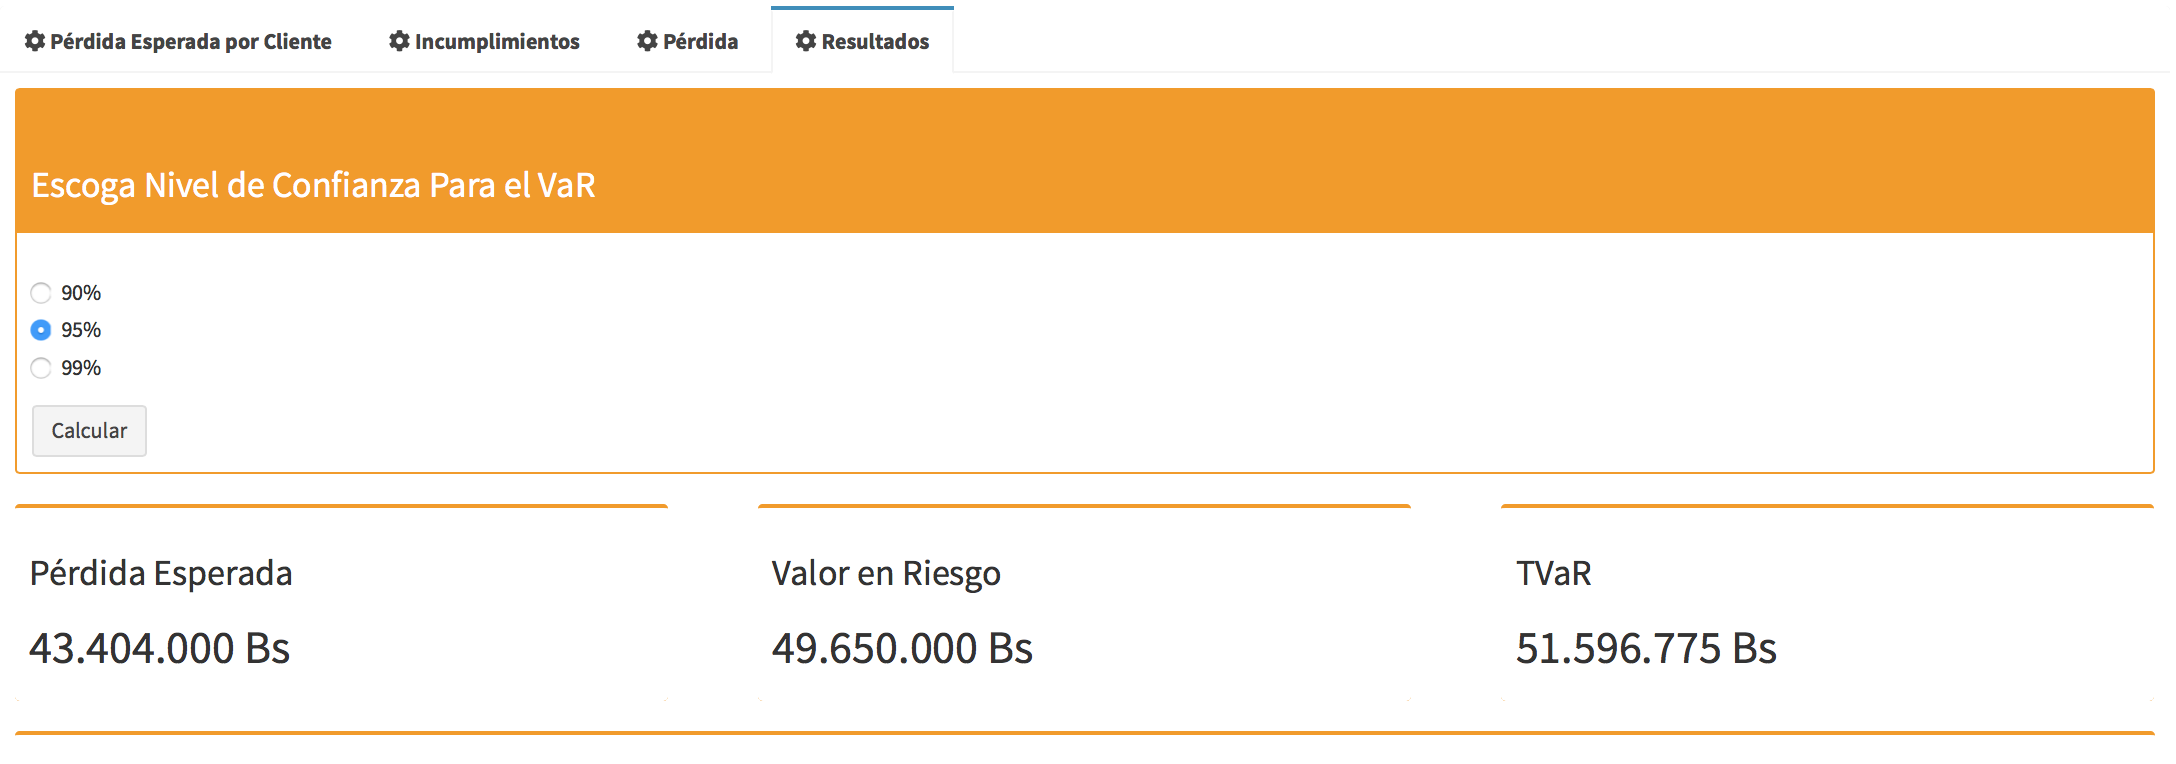
\includegraphics{images/45.png}
\caption{\label{fig:"sd"}}
\end{figure}

\hypertarget{strestesting}{%
\subsection{StresTesting}\label{strestesting}}

En esta sección se muestra el valor de una prueba de estres en la metodología.

\begin{figure}
\centering

\includegraphics{images/46.png}
\caption{\label{fig:"sd"}}
\end{figure}

\hypertarget{creditmetric-1}{%
\section{CreditMetric}\label{creditmetric-1}}

En esta sección se presenta la segunda metodología de riesgo de crédito.

\begin{figure}
\centering
\includegraphics{images/47.png}
\caption{\label{fig:"sd"}}
\end{figure}

\hypertarget{simulacion-y-resultados}{%
\subsection{Simulación y Resultados}\label{simulacion-y-resultados}}

En esta sección debemos seleccionar el número de simulaciones para iniciar el cálculo de la metodología.

\begin{figure}
\centering
\includegraphics{images/48.png}
\caption{\label{fig:"sd"}}
\end{figure}

Una vez iniciada la simulación obtendremos el histograma de las pérdidas simuladas y las métricas de riesgo.

\begin{figure}
\centering
\includegraphics{images/49.png}
\caption{\label{fig:"sd"}}
\end{figure}

\hypertarget{stresstesting}{%
\subsection{StressTesting}\label{stresstesting}}

En esta sección realizaremos una prueba de estres a la metodología CreditMetrics.

\begin{figure}
\centering
\includegraphics{images/50.png}
\caption{\label{fig:"sd"}}
\end{figure}

\hypertarget{backtesting-1}{%
\section{BackTesting}\label{backtesting-1}}

En esta sección se harán pruebas sobre el VaR, usando el test de Haas, Kupiec y el mixto

\begin{figure}
\centering
\includegraphics{images/51.png}
\caption{\label{fig:"sd"}}
\end{figure}

\hypertarget{indicadores-contables-1}{%
\section{Indicadores Contables}\label{indicadores-contables-1}}

En esta última sección se calcularán ciertos indicadores contables, algunos basados únicamente en los datos contables y otros basados en las métricas de riesgo.

\begin{figure}
\centering
\includegraphics{images/52.png}
\caption{\label{fig:"sd"}}
\end{figure}

\cleardoublepage

\hypertarget{appendix-apendice}{%
\appendix \addcontentsline{toc}{chapter}{\appendixname}}


\hypertarget{formato-de-los-datos-de-la-aplicacion}{%
\chapter{Formato de los datos de la aplicación}\label{formato-de-los-datos-de-la-aplicacion}}

En esta sección se describirá el formato que deben poseer los datos que necesitará la aplicación.

\hypertarget{score-y-rating-1}{%
\section{Score y Rating}\label{score-y-rating-1}}

Este módulo esta compuesto de 4 pestañas:

\hypertarget{scoring-1}{%
\subsection{Scoring}\label{scoring-1}}

Este archivo debe tener la extensión \emph{.txt} ó \emph{csv}. Todos sus campos deben ser numéricos, en caso de haber categorías deben estar expresadas en números. Esta data es escencial para la contrucción del modelo de Scoring.

\begin{itemize}
\tightlist
\item
  Una de sus columnas deben tener el nombre ``Creditability''

  \begin{itemize}
  \tightlist
  \item
    Para clientes en Default 1
  \item
    Para clientes en regla 0
  \end{itemize}
\end{itemize}

\hypertarget{proyeccion-scoring-1}{%
\subsection{Proyección Scoring}\label{proyeccion-scoring-1}}

En esta sección se realizan predicciones a partir del modelo Score calculado. Los campos de los datos deben ser exatamente igual a los de los datos de entrenamiento, con la excepción de que el campo ``Creditability'' no debería existir.

\hypertarget{rating-1}{%
\subsection{Rating}\label{rating-1}}

Archivo con extensión \emph{.csv} ó \emph{.txt} el cual debe estar conformado por dos campos:

\begin{itemize}
\tightlist
\item
  pd: Campo numérico indicando probabilidad de incumplimiento
\item
  r: Campo categórico que indica rating del cliente
\end{itemize}

\hypertarget{proyeccion-rating-1}{%
\subsection{Proyección Rating}\label{proyeccion-rating-1}}

Archivo con extensión \emph{.csv} ó \emph{.txt} el cual debe tener una única entrada numérica entre 0 y 1 correspondiente a la probabilidasd de incumplimiento.

\hypertarget{perdida-por-incumplimiento-2}{%
\section{Pérdida por incumplimiento}\label{perdida-por-incumplimiento-2}}

\hypertarget{perdida-por-cliente-1}{%
\subsection{Pérdida por cliente}\label{perdida-por-cliente-1}}

Archivo con extensión \emph{.csv} ó \emph{.txt} el cual debe tener una única data numérica entre 0 y 1 correspondiente al porcentaje de pérdida luego del Default.

\hypertarget{perdida-por-cliente-2}{%
\subsection{Pérdida por cliente}\label{perdida-por-cliente-2}}

Archivo con extensión \emph{.csv} ó \emph{.txt} el cual debe tener dos campos

\begin{itemize}
\item
  clases: Variable categórica correspondiente a las clases crediticias
\item
  perdida: variable numérica entre 0 y 100 correspondiente a la pérdida por clase
\end{itemize}

\hypertarget{matriz-de-transicion-4}{%
\section{Matriz de transición}\label{matriz-de-transicion-4}}

\hypertarget{migraciones-historicas}{%
\subsection{Migraciones históricas}\label{migraciones-historicas}}

Archivo con extensión \emph{.csv} ó \emph{.txt} el cual debe tener dos campos

\begin{itemize}
\item
  inicio: Variable categórica correspondiente a la clase inicial del cliente
\item
  fin: Variable categórica correspondiente a la clase final del cliente
\end{itemize}

\hypertarget{creditrisk-3}{%
\section{CreditRisk+}\label{creditrisk-3}}

\hypertarget{exposicion-2}{%
\subsection{Exposición}\label{exposicion-2}}

Archivo con extensión \emph{.csv} ó \emph{.txt} el cual debe tener una única data numérica correspondiente al valor deudor del crédito.

\hypertarget{probabilidad-de-incumplimiento-1}{%
\subsection{Probabilidad de incumplimiento}\label{probabilidad-de-incumplimiento-1}}

Archivo con extensión \emph{.csv} ó \emph{.txt} el cual debe tener una única data numérica correspondiente a la probabilidad de incumplimiento de cada cliente.

\hypertarget{perdidas-dado-el-incumplimiento-2}{%
\subsection{Pérdidas dado el incumplimiento}\label{perdidas-dado-el-incumplimiento-2}}

Archivo con extensión \emph{.csv} ó \emph{.txt} el cual debe tener una única data numérica correspondiente a la pérdida esperada por cliente en pocentaje de 0 a 1.

\hypertarget{creditmetrics-1}{%
\section{CreditMetrics}\label{creditmetrics-1}}

\hypertarget{exposicion-3}{%
\subsection{Exposición}\label{exposicion-3}}

Archivo con extensión \emph{.csv} ó \emph{.txt} el cual debe tener dos campos:

\begin{itemize}
\item
  creditos: Variable numérica correspondiente al monto del crédito restante a pagar por el cliente.
\item
  calif: Variable categórica correspondiente a la clasificación crediticia del cliente.
\end{itemize}

\hypertarget{martriz-de-transicion}{%
\subsection{Martriz de transición}\label{martriz-de-transicion}}

Archivo con extensión \emph{.csv} ó \emph{.txt} el cual debe poseer :

\begin{itemize}
\item
  Un campo con nombre \emph{inicio/fin} con las categorias crediticias
\item
  Una matriz numérica correspondiente a las probabilidades de transición entre clases, la suma de cada columna debe ser 1.
\end{itemize}

\hypertarget{perdida-por-clase-1}{%
\subsection{Pérdida por clase}\label{perdida-por-clase-1}}

Archivo con extensión \emph{.csv} ó \emph{.txt} el cual debe poseer los siguientes campos:

\begin{itemize}
\item
  Clase: Variable categórica con las distintas clases crediticias.
\item
  Pérdida esperada: variable numérica entre 0 y 100 correspondiente a la pérdida esperada por cliente
\item
  Mínimo esperado: variable numérica entre 0 y 100 correspondiente a la mínima pérdida esperada por cliente
\item
  Máximo esperado: variable numérica entre 0 y 100 correspondiente a la máxima pérdida esperada por cliente
\end{itemize}

\hypertarget{backtesting-2}{%
\section{BackTesting}\label{backtesting-2}}

Archivo con extensión \emph{.csv} ó \emph{.txt} el cual debe poseer los siguientes campos:

\begin{itemize}
\tightlist
\item
  Fecha en formato dia/mes/año (27/03/2018)
\item
  Valor numérico que contenga la información del VaR de ese día
\item
  Valor numérico que contenga el valor nominal del portafolio
\end{itemize}

Es importante mencionar que el archivo debe contener 252 observaciones

\hypertarget{indicadores-contables-2}{%
\section{Indicadores Contables}\label{indicadores-contables-2}}

Archivo con extensión \emph{.csv} ó \emph{.txt} el cual debe poseer los siguientes 2 campos:

\begin{itemize}
\tightlist
\item
  concepto: Nombre de los diferentes indicadores:

  \begin{itemize}
  \tightlist
  \item
    Saldo de la Cartera de Crédito vencida al cierre del periodo
  \item
    Saldo de la Cartera de Crédito total al cierre del periodo
  \item
    Saldo de la estimación preventiva para riesgos crediticios al cierre del periodo
  \item
    Resultado contable de los activos financieros
  \end{itemize}
\item
  Valor: Variable numérica que refleja el valor contable.
\end{itemize}

\end{document}
